% ch12a Superconductivity in metals, part a (书页 189-204 / 分册p001-016)
% 第12章 Superconductivity in metals
\chapter{金属中的超导电性}

本章中，我们聚焦于超导电性现象及其背后的巴丁–库珀–施里弗（Bardeen–Cooper–Schrieffer，BCS）理论（文献 [BCS1957]）。当金属中有限比例的传导电子凝聚到一个由单一量子力学相位所表征的量子态上时，超导电性便出现了。这一量子力学相位的取值因超导体而异。把数量级达阿伏伽德罗常量之多的电子的相位锁定在一起，保证了超导态的刚性。例如，凝聚体中的电子不可能个别地运动；整个凝聚体作为一个单一的整体从样品的一端移动到另一端。同样，旨在破坏凝聚体的电子散射事件必须扰乱宏观数目电子的相位，才能摧毁超导态。因此，相位刚性既意味着超导凝聚体的集体运动，也意味着它的集体性毁灭。唯一另一个源于把宏观数目的粒子凝聚到相位锁定态的物理现象是玻色–爱因斯坦凝聚。然而，这两种效应之间有一个关键差别：构成超导凝聚体的粒子是库珀对（Cooper pair），它并不服从玻色统计。事实上，正是作用于组成库珀对的电子之上的泡利原理，阻止了把超导问题完全映射为一个简单的玻色凝聚问题。正如我们将看到的，正是泡利原理使 BCS 理论如此有效。这话是什么意思？在 BCS 理论中，假设电子形成库珀对，而且各对之间强烈地相互交叠。如此强的交叠本应意味着对与对之间存在强关联。事实上，正是对间的关联解释了超导体大多数可观测的性质，例如能隙和迈斯纳效应。然而在 BCS 理论中，库珀对之间并没有明确的动力学相互作用。唯一的相互作用——如果可以这样理解的话——来自泡利不相容原理，它禁止两个库珀对占据同一动量态。BCS 理论如此有效，这一事实深刻地揭示了金属中对–对关联的真实本质。它暗示金属中真实的对–对相互作用主要源于泡利不相容原理，而不是某种附加的动力学相互作用。正是主要因为这个原因，BCS 的简单配对假设才取得了如此深刻的成功。

\section{超导电性：唯象描述}

首先，我们摆明任何超导理论都必须解释的实验事实。

\begin{figure}[H]\centering
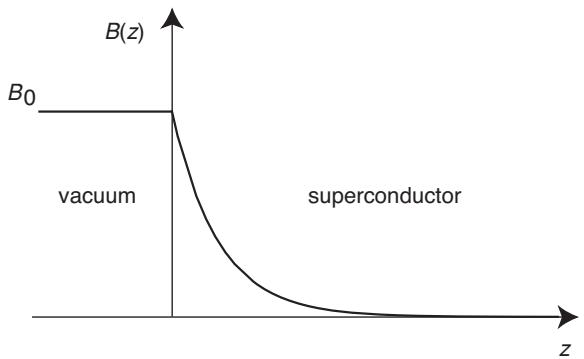
\includegraphics[width=0.5\textwidth]{figs/ch12/fig_12.1.jpg}
\caption*{图 12.1\quad 第I类超导体中磁场的衰减。}\label{fig:auto:12.1}
\end{figure}

\begin{figure}[H]\centering
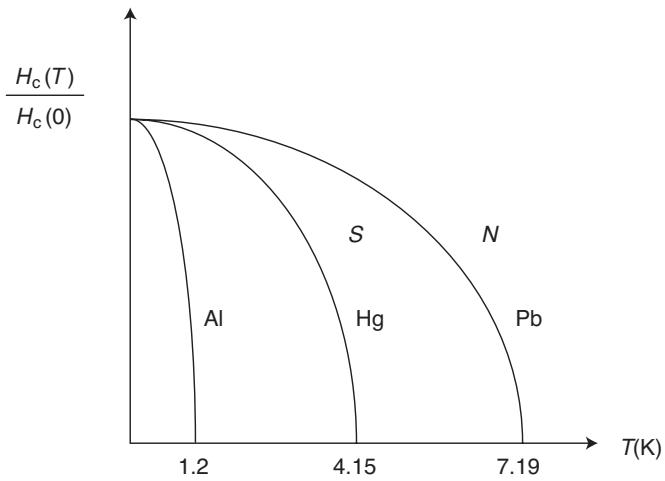
\includegraphics[width=0.55\textwidth]{figs/ch12/fig_12.2.jpg}
\caption*{图 12.2\quad 临界场随温度的依赖关系。横轴上标示的温度是一系列金属的超导转变温度。}\label{fig:auto:12.2}
\end{figure}

\textbf{(a) 零电阻}\quad 超导电性最典型的标志，是电阻在某个临界温度 $T_{\mathrm{c}}$ 以下消失。超导态是一个热力学上截然不同的物态。在 $T_{\mathrm{c}}$ 以下，电流的流动没有任何损耗。在高 $T_{\mathrm{c}}$ 材料被制备出来之前，铌（Nb）保持着最高的转变温度 $9.26\,\mathrm{K}$。

\textbf{(b) 迈斯纳效应}\quad 另一个特征是对磁场的排斥，即迈斯纳效应（Meissner effect）。迈斯纳效应完全的材料称为第I类超导体。因此，第I类超导体的内部是一个完全抗磁体。加在第I类超导体边界上的磁场，在材料内部随距离按指数衰减，如图12.1所示。穿透深度（penetration depth）$\lambda_{L}$ 定义为磁场衰减到 $1/e$ 倍所经过的距离。在 $T_{\mathrm{c}}$ 以下，破坏超导电性所需的场增大到某个临界值 $H_{\mathrm{c}}(T)$，如图12.2所示。由于超导体内部的磁场为零，
\begin{equation*}
B=0=H_{\mathrm{appl}}+4\pi M,\tag{12.1}
\end{equation*}
其中 $H_{\mathrm{appl}}$ 是外加场，$M$ 是磁化强度。解此方程，我们得到磁化强度为
\begin{equation*}
M=-\frac{1}{4\pi}H_{\mathrm{appl}}.\tag{12.2}
\end{equation*}
$M$ 的负值表明超导体内部是抗磁的。在低于 $T_{\mathrm{c}}$ 的任何温度下，磁化强度都应当是外加场的线性函数。具有这种形式磁化强度的材料称为第I类超导体。正常态用 N 表示，超导态用 S 表示。在 $H_{\mathrm{c}}$ 以上，$B\neq 0$，磁化强度不再服从式 (12.2)。

\begin{figure}[H]\centering
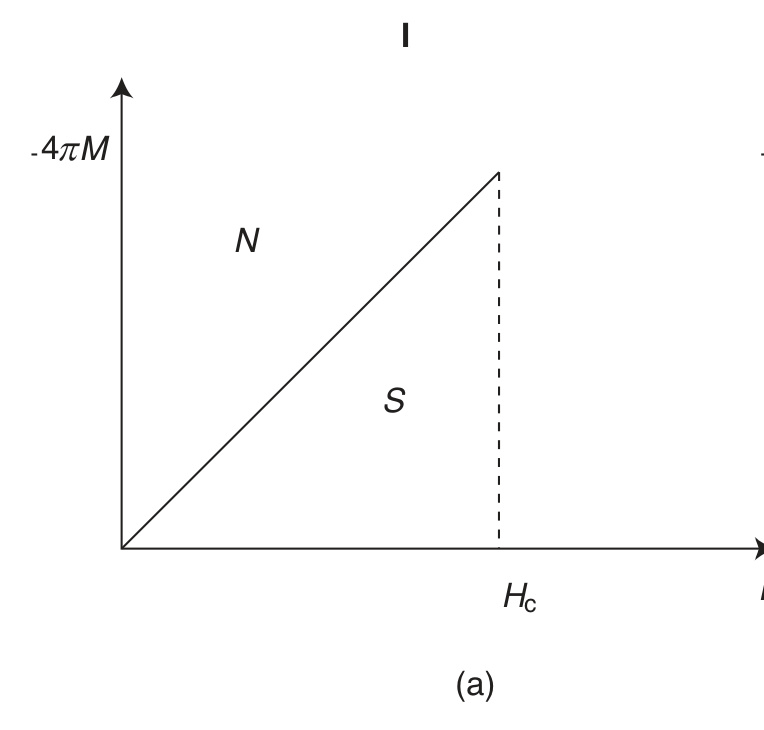
\includegraphics[width=0.48\textwidth]{figs/ch12/fig_12.3_a.jpg}\hfill
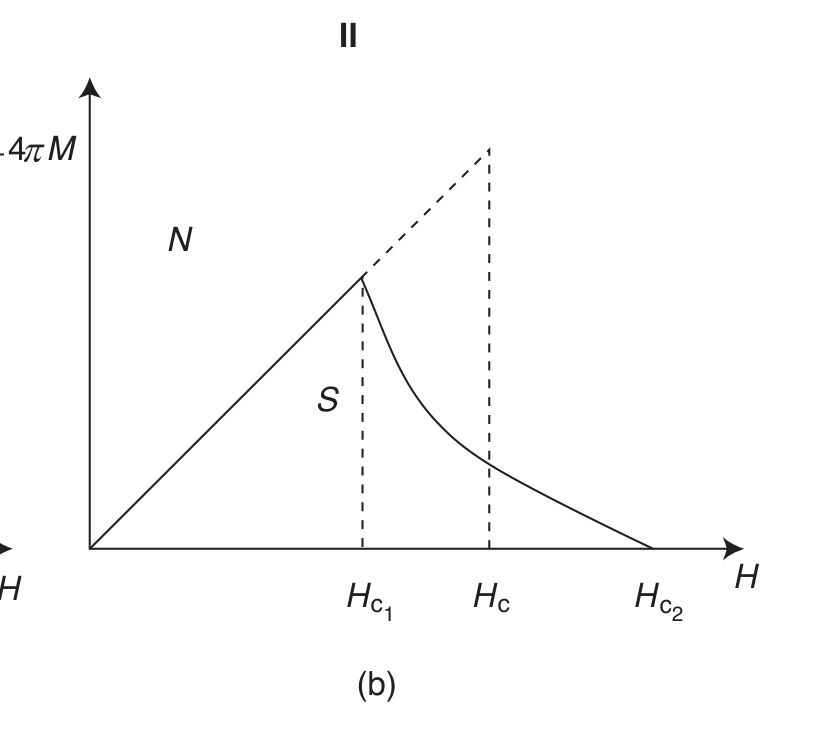
\includegraphics[width=0.48\textwidth]{figs/ch12/fig_12.3_b.jpg}
\caption*{图 12.3\quad (a) 第I类超导体的磁化强度对外加场的关系。(b) 第II类超导体的磁化强度对外加场的关系。在 $H_{\mathrm{c}_1}$ 与 $H_{\mathrm{c}_2}$ 之间，磁力线穿入超导体但并不破坏超导电性。磁力线形成一个涡旋晶格。}\label{fig:auto:12.3}
\end{figure}

在某些材料中，超导电性可以保持到上临界场 $H_{\mathrm{c}_2}$，但在下临界场 $H_{\mathrm{c}_1}$ 与 $H_{\mathrm{c}_2}$ 之间观察到的是不完全的迈斯纳效应。由此得到的磁化强度如图12.3(b)所示。表现出这种磁化强度的材料称为第II类超导体。在 $H_{\mathrm{c}_1}$ 与 $H_{\mathrm{c}_2}$ 之间，磁场穿入材料但超导电性并未被破坏。磁力线形成一个规则排列，称为阿布里科索夫（Abrikosov）涡旋晶格（文献 [A1957]）。所有高 $T_{\mathrm{c}}$ 铜氧化物超导体都是第II类的。

我们主要关心第I类材料。为理解超导体中的穿透深度，我们求助于伦敦（London）方程。首先，我们需要电场旋度的麦克斯韦方程：$-\partial\mathbf{B}/\partial t=c\nabla\times\mathbf{E}=c\rho\nabla\times\mathbf{J}$，其中 $\rho$ 是电阻率。在理想导体中 $\rho=0$，因而 $\partial\mathbf{B}/\partial t=0$。超导体中同样有 $\rho=0$。然而，实验事实是超导体内部 $B=0$。这一结果无法从麦克斯韦方程推出。正是迈斯纳效应把超导电性与仅显示理想导电性的材料区分开来。在超导体内部，磁通的排出由流动的电流所介导。伦敦于1935年提出，在超导体中处处有
\begin{equation*}
\mathbf{J}=-\mathrm{const.}\,\mathbf{A},\tag{12.3}
\end{equation*}
其中 $\mathbf{A}$ 是矢量势，$\mathbf{B}=\nabla\times\mathbf{A}$。由这个拟设（ansatz）出发，伦敦得以证明磁场在超导体内部按指数衰减。从量纲上看，该常数具有 $1/(L\cdot\text{时间})$ 的单位。我们把这个常数写成
\begin{equation*}
\mathrm{const.}=\frac{c}{4\pi\lambda_{L}^{2}},\tag{12.4}
\end{equation*}
其中 $c$ 是光速。对式 (12.3) 两边取旋度，我们得到
\begin{equation*}
\nabla\times\mathbf{J}=-\frac{c}{4\pi\lambda_{L}^{2}}\mathbf{B}.\tag{12.5}
\end{equation*}
由安培定律
\begin{equation*}
\nabla\times\mathbf{B}=\frac{4\pi}{c}\mathbf{j},\tag{12.6}
\end{equation*}
我们得到
\begin{equation*}
\nabla\times\left(\nabla\times\mathbf{B}\right)=\frac{4\pi}{c}\nabla\times\mathbf{J},\tag{12.7}
\end{equation*}
这意味着
\begin{equation*}
\nabla^{2}\mathbf{B}=\frac{1}{\lambda_{L}^{2}}\mathbf{B}.\tag{12.8}
\end{equation*}
此方程的解
\begin{equation*}
B(r)=B(0)\mathrm{e}^{-r/\lambda_{L}},\tag{12.9}
\end{equation*}
是在长度尺度 $\lambda_{L}$ 上按指数衰减的磁感应强度。磁场在超导体内的指数衰减就是迈斯纳效应。令 $v_{\mathrm{s}}$、$m^{*}$ 与 $e^{*}$ 分别是超导体中载流子的速度、质量和电荷。于是
\begin{equation*}
m^{*}\dot{\mathbf{v}}_{\mathrm{s}}=-e^{*}\mathbf{E}.\tag{12.10}
\end{equation*}
这些电子的电流定义为 $\mathbf{J}=-e^{*}\mathbf{v}_{\mathrm{s}}n_{\mathrm{s}}$，将它与式 (12.10) 联立，得到电流的时间演化方程
\begin{equation*}
\frac{\partial\mathbf{J}}{\partial t}=\frac{n_{\mathrm{s}}e^{*2}}{m^{*}}E\tag{12.11}
\end{equation*}
对两边取旋度，我们发现
\begin{align*}
0&=\frac{\partial}{\partial t}\left(\nabla\times\mathbf{J}\right)-\frac{n_{\mathrm{s}}e^{2}}{m^{*}}\nabla\times\mathbf{E}\\
&=\frac{\partial}{\partial t}\left(\nabla\times\mathbf{J}+\frac{n_{\mathrm{s}}e^{*2}}{m^{*}c}\mathbf{B}\right).\tag{12.12}
\end{align*}
将式 (12.12) 与式 (12.5) 比较，我们得到穿透深度为
\begin{equation*}
\lambda_{L}=\left(\frac{m^{*}c^{2}}{4\pi n_{\mathrm{s}}e^{*2}}\right)^{1/2}.\tag{12.13}
\end{equation*}
于是我们看到，随着超导密度的增大，$\lambda_{L}$ 减小。

我们可以借助金兹堡（Ginsburg）和朗道（Landau）的理论（文献 [GL1950]）来论证伦敦方法中的主要假设。这一唯象理论的关键之处在于：超导态与正常态之间自由能密度之差可以写成超导态序参量 $\psi(\mathbf{r})$ 的泛函。物理上，$|\psi(\mathbf{r})|^{2}$ 正比于超导态中的电荷密度 $n_{\mathrm{s}}$。因此，我们可以把 $\psi(\mathbf{r})$ 解释为超导态的波函数。在 BCS 理论中，$\psi(\mathbf{r})$ 扮演库珀对质心波函数的角色。在 $T_{\mathrm{c}}$ 附近，超流密度很小，故 $|\psi|^{2}\ll n_{\mathrm{e}}$。于是，金兹堡和朗道把超导态在 $T_{\mathrm{c}}$ 附近的自由能密度按 $|\psi|^{2}$ 的幂级数展开为
\begin{equation*}
F=F_{\mathrm{N}}+\int\mathrm{d}\mathbf{r}\left(\frac{\hbar^{2}}{2m^{*}}|\nabla\psi|^{2}+a(T)|\psi(\mathbf{r})|^{2}+b(T)|\psi(\mathbf{r})|^{4}\right),\tag{12.14}
\end{equation*}
其中保留了动能项 $|\nabla\psi|^{2}$，以显式地计入场 $\psi(\mathbf{r})$ 的空间变化。正常态的自由能是 $F_{\mathrm{N}}$。系数 $a(T)$ 与 $b(T)$ 是实的且依赖于温度，并且为使体系稳定，要求 $b(T)>0$。

为求系统的基态，我们对 $\psi^{*}(\mathbf{r})$ 极小化自由能密度：
\begin{equation*}
-\frac{\hbar^{2}}{2m^{*}}\nabla^{2}\psi(\mathbf{r})+a(T)\psi(\mathbf{r})+2b(T)|\psi(\mathbf{r})|^{2}\psi(\mathbf{r})=0.\tag{12.15}
\end{equation*}
由于自由能密度中含有恒为正的 $|\nabla\psi|^{2}$ 项，自由能的极小化要求 $\nabla\psi(\mathbf{r})=0$，或者说 $\psi$ 在空间中均匀。因此，鞍点方程的解要么是 $\psi=0$，要么是
\begin{equation*}
|\psi_{0}|^{2}=-\frac{a(T)}{2b(T)}=n_{\mathrm{s}},\tag{12.16}
\end{equation*}
这意味着 $a(T)<0$。倘若 $a(T)$ 大于零，则 $\psi=0$，系统将处于正常态。由于超导电性在 $T_{\mathrm{c}}$ 处消失，必须有 $a(T_{\mathrm{c}})=0$。把 $a(T)$ 在 $T_{\mathrm{c}}$ 附近作一阶泰勒展开，得到
\begin{equation*}
a(T)=a_{1}(T-T_{\mathrm{c}})\tag{12.17}
\end{equation*}
其中 $a_{1}>0$。

回忆起存在矢量势 $\mathbf{A}$ 时的电流密度为
\begin{equation*}
\mathbf{J}=\frac{e^{*}\hbar}{2\mathrm{i}m^{*}}\left(\psi^{*}\nabla\psi-\psi\nabla\psi^{*}\right)-\frac{e^{*2}}{m^{*}c}|\psi|^{2}\mathbf{A}.\tag{12.18}
\end{equation*}
若假定磁场足够小，以致 $\psi_{0}$ 的平衡值不变，则把 $\psi_{0}$ 代入式 (12.18) 便得到伦敦结果
\begin{equation*}
\mathbf{J}=-\frac{e^{*2}n_{\mathrm{s}}}{m^{*}c}\mathbf{A}.\tag{12.19}
\end{equation*}
利用式 (12.13)，我们发现这一结果与式 (12.4) 一致。于是，从这个简单的唯象方法出发，我们能够论证电流密度的伦敦拟设。的确，正如我们将看到的，BCS 超导理论的核心思想内容，正如在金兹堡–朗道理论中那样，是存在一个序参量，它描述一个具有确定相位的电荷 $2e$ 凝聚体。这样的凝聚体破坏 $U(1)$ 规范对称性，正如第1章所讨论的。事实上，迈斯纳效应的存在本身就意味着一个连续对称性的破缺。磁场无法穿入超导体这一事实立即告诉我们：在超导体中，光子是有质量的。因此，不能再假定电子是传播的自由度。实际上，在超导体中它们确实不是。电荷以 $2e$ 为单位量子化，这意味着 $U(1)$ 对称性发生了破缺。

\textbf{(c) 热容}\quad 在超导态中，熵连续但急剧地下降，标志着一种高度有序状态的形成。这描绘在图12.4(a)中。因此，熵对温度的导数在转变的超导一侧必然比正常一侧更陡。于是，热容在 $T_{\mathrm{c}}$ 处不连续，超导电性是一个二级相变。如图12.4(b)所示，在超导态中，热容 $c_{\mathrm{s}}$ 按 $c_{\mathrm{s}}\propto\exp(-\Delta/k_{\mathrm{B}}T)$ 衰减，其中 $\Delta$ 是一个能量尺度。这种形式的热容表明激发谱中存在能隙，且 $\epsilon_{p}>\mu$。让我们用一个简单的计算来验证这一点：
\begin{equation*}
c_{\mathrm{V}}=\frac{\partial}{\partial T}\int\frac{\epsilon_{p}\,\mathrm{d}\epsilon_{p}}{\left(\mathrm{e}^{\beta(\epsilon_{p}-\mu)}+1\right)}\overset{T\to 0}{\longrightarrow}\frac{\partial}{\partial T}\int\epsilon_{p}\,\mathrm{e}^{-\beta(\epsilon_{p}-\mu)}\,\mathrm{d}\epsilon_{p}.\tag{12.20}
\end{equation*}
若 $(\epsilon_{p}-\mu)\approx\Delta$，则 $c_{\mathrm{V}}\sim\exp(-\Delta(T=0)/k_{\mathrm{B}}T)$。因此，在超导态中，我们采用图12.5所示的能隙图像。

超导态中费米能级处能隙的形成导致系统基态能量的降低。能隙实际上是 $2\Delta$ 而非 $\Delta$。因此，$\epsilon_{p}-\mu$ 只占能隙的一半。实验上，能隙可以通过隧穿或超声衰减实验来测量。从热力学上看，能隙引起热容的不连续，即 $c_{\mathrm{s}}(T_{\mathrm{c}}^{-})-c_{\mathrm{N}}(T_{\mathrm{c}}^{+})\neq 0$。跨越超导转变时，自由能的两个一阶导数都为零，因此超导转变没有潜热。在 $T_{\mathrm{c}}$ 以上 $\Delta=0$，而在 $T=0$ 时 $\Delta$ 取其最大值。$\Delta(T)/\Delta(T=0)$ 的典型图像示于图12.6。弱耦合超导体的比值 $2\Delta(T=0)/k_{\mathrm{B}}T_{\mathrm{c}}$ 在 1 到 3 之间；强耦合对应于 $2\Delta(T=0)/k_{\mathrm{B}}T_{\mathrm{c}}>4$。在超导体中产生一个电子–空穴对所需的基本能量尺度是 $2\Delta$。

\begin{figure}[H]\centering
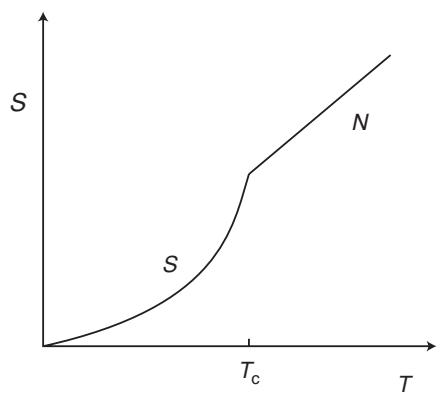
\includegraphics[width=0.48\textwidth]{figs/ch12/fig_12.4_a.jpg}\hfill
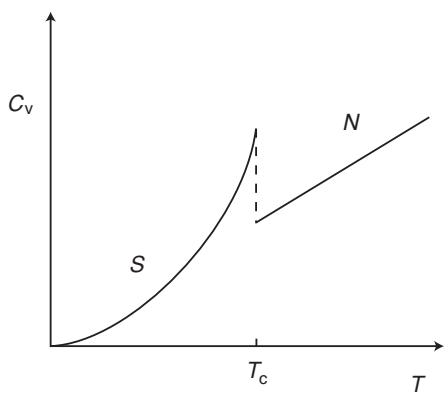
\includegraphics[width=0.48\textwidth]{figs/ch12/fig_12.4_b.jpg}
\caption*{图 12.4\quad (a) 熵在超导转变两侧的行为。(b) 正常态与超导态中热容的行为。}\label{fig:auto:12.4}
\end{figure}

\begin{figure}[H]\centering
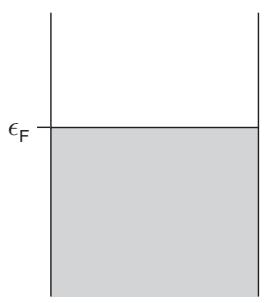
\includegraphics[width=0.42\textwidth]{figs/ch12/fig_12.5_a.jpg}\hfill
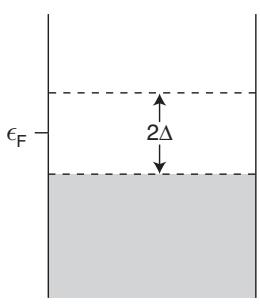
\includegraphics[width=0.42\textwidth]{figs/ch12/fig_12.5_b.jpg}
\caption*{图 12.5\quad (a) 正常态中被填满的能级。(b) 超导态中能隙的形成。完整的能隙是 $2\Delta$，而非 $\Delta$。}\label{fig:auto:12.5}
\end{figure}

\textbf{(d) 微波与红外性质}\quad 由于能隙的存在，能量小于 $2\Delta$ 的光子不会被吸收：所有这样的光子都被反射。当 $\omega<2\Delta(T=0)/\hbar$ 时发生完全反射。该条件成立时，光子看到的是一个完全无阻的表面。绝对零度下当 $\omega>2\Delta(T=0)/\hbar$ 时，电阻开始趋近正常态的值。我们在假定弱耦合描述对超导体适用的前提下估计这一能量：于是 $\Delta\sim 2k_{\mathrm{B}}T_{\mathrm{c}}$，而 $\omega\sim 4k_{\mathrm{B}}T_{\mathrm{c}}/\hbar$。对于 $T_{\mathrm{c}}=5\,\mathrm{K}$，$\omega\sim 10^{12}\,\mathrm{s}^{-1}$。这一频率位于红外波段。因此红外辐射可以穿入超导体并散射电子。

\begin{figure}[H]\centering
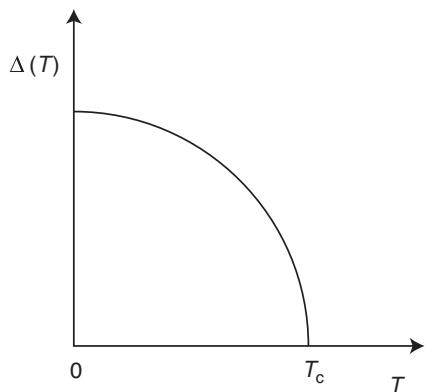
\includegraphics[width=0.5\textwidth]{figs/ch12/fig_12.6.jpg}
\caption*{图 12.6\quad 超导能隙 $\Delta$ 随 $T\to T_{\mathrm{c}}$ 的行为。}\label{fig:auto:12.6}
\end{figure}

\begin{figure}[H]\centering
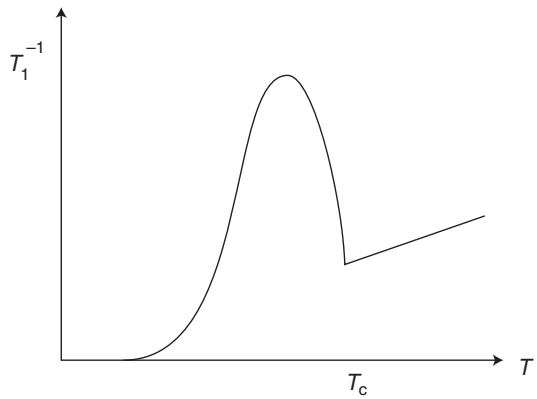
\includegraphics[width=0.5\textwidth]{figs/ch12/fig_12.7.jpg}
\caption*{图 12.7\quad $T_{\mathrm{c}}$ 处及 $T_{\mathrm{c}}$ 以下自旋–晶格弛豫时间的行为。$1/T_{1}$ 的增强是超导体中自旋协同行动的标志。}\label{fig:auto:12.7}
\end{figure}

\textbf{(e) 超声衰减}\quad 当 $\omega_{\mathbf{q}}<2\Delta/\hbar$ 时，入射声子束观察不到阻尼。与微波吸收的情形一样，$\omega_{\mathbf{q}}$ 必须超过产生一个电子–空穴对所需的能量。

\textbf{(f) 核自旋弛豫}\quad 考虑一组被强迫沿磁场排列的原子核。平衡磁化强度恢复的速率称为自旋–晶格弛豫速率 $1/T_{1}$。在超导体中，恰在 $T_{\mathrm{c}}$ 以下有 $\left(1/T_{1}\right)_{\mathrm{S}}>\left(1/T_{1}\right)_{\mathrm{N}}$。也就是说，超导态的形成带来弛豫速率的增强。Hebel 和 Slichter 最先在实验上观察到这一效应（文献 [HS1959]）。恰在 $T_{\mathrm{c}}$ 以下弛豫速率的峰称为 Hebel–Slichter 峰。

\textbf{(g) 同位素效应}\quad 实验上观察到，若以同位素方式改变离子的质量，$T_{\mathrm{c}}$ 会相应改变：
\begin{equation*}
T_{\mathrm{c}}\propto\frac{1}{\sqrt{M}}\propto\omega_{\mathrm{D}}.\tag{12.21}
\end{equation*}
这一观察表明，电子–声子耦合处于超导电性的核心（至少对传统超导电性是如此）。

\section{电子–声子有效相互作用}

$T_{\mathrm{c}}$ 的同位素依赖性证实了电子–声子耦合处于超导电性机制的中心。现在我们展示电子–声子耦合如何在两个电子之间产生吸引相互作用。我们分析的出发点是一个有序的电子能带，其中动能为 $\epsilon_{\mathbf{k}}$ 的电子与晶体的量子化振动模式相耦合。于是，我们的哈密顿量 $H=H_{o}+H_{\mathrm{e}\text{-}\mathrm{ph}}$ 由一个有序部分
\begin{equation*}
H_{o}=\sum_{\mathbf{q}}\hbar\omega_{\mathbf{q}}b_{\mathbf{q}}^{\dagger}b_{\mathbf{q}}+\sum_{\mathbf{k}}\epsilon_{\mathbf{k}}a_{\mathbf{k}}^{\dagger}a_{\mathbf{k}},\tag{12.22}
\end{equation*}
与电子–晶格相互作用
\begin{equation*}
H_{\mathrm{e}\text{-}\mathrm{ph}}=\sum_{\mathbf{k},\mathbf{q}}M_{\mathbf{q}}a_{\mathbf{k}+\mathbf{q}}^{\dagger}a_{\mathbf{k}}\bigl(b_{\mathbf{q}}+b_{-\mathbf{q}}^{\dagger}\bigr)\tag{12.23}
\end{equation*}
之和构成。

电子–声子耦合常数定义于第11.3节。我们将假定电子–声子相互作用是弱的，并对该相互作用做二阶微扰论。作为二阶微扰，我们预期电子–声子相互作用将给能量带来一个负的修正。虽然最终结果用二阶微扰论即可相当直接地建立起来（见习题12.3），但我们将采用相似变换（similarity transformation），因为该方法在电子–声子问题中有众多应用。我们的分析将仿照 Schrieffer–Wolff 变换。消去线性的电子–声子相互作用将产生一个二阶的相互作用，由此我们将能够推导出声子在何种条件下有效地束缚电子。

我们寻找一个变换 $S$，使得
\begin{equation*}
\left[H_{o},S\right]=-H_{\mathrm{e}\text{-}\mathrm{ph}}.\tag{12.24}
\end{equation*}
变换后的哈密顿量将为
\begin{align*}
\tilde{H}&=\mathrm{e}^{-S}H\mathrm{e}^{S}\\
&=H_{o}+\frac{1}{2}\left[H_{\mathrm{e}\text{-}\mathrm{ph}},S\right]+\cdots.\tag{12.25}
\end{align*}
我们设定 $S$ 具有如下形式
\begin{equation*}
S=\sum_{\mathbf{k},\mathbf{q}}\bigl(A_{\mathbf{k},\mathbf{q}}b_{-\mathbf{q}}^{\dagger}+B_{\mathbf{k},\mathbf{q}}b_{\mathbf{q}}\bigr)M_{\mathbf{q}}a_{\mathbf{k}+\mathbf{q}}^{\dagger}a_{\mathbf{k}},\tag{12.26}
\end{equation*}
其中 $A$ 与 $B$ 有待由式 (12.24) 的约束确定。为继续推进，我们需要对易关系
\begin{align*}
&\left[n_{\mathbf{k}},a_{\mathbf{k}_{1}}^{\dagger}a_{\mathbf{k}_{2}}\right]=a_{\mathbf{k}_{1}}^{\dagger}a_{\mathbf{k}_{2}}\left(\delta_{\mathbf{k}_{1}\mathbf{k}}-\delta_{\mathbf{k}_{2}\mathbf{k}}\right),\\
&\qquad\quad\ \left[b_{\mathbf{q}}^{\dagger},b_{\mathbf{q}}\right]=-1,\\
&\qquad\quad\ \left[b_{\mathbf{q}}^{\dagger}b_{\mathbf{q}},b_{\mathbf{q}'}\right]=-b_{\mathbf{q}}\delta_{\mathbf{q}\mathbf{q}'}.\tag{12.27}
\end{align*}
于是我们得到
\begin{align*}
\left[H_{o},S\right]&=\sum_{\mathbf{q}',\mathbf{k},\mathbf{q}}\hbar\omega_{\mathbf{q}'}\left[b_{\mathbf{q}}^{\dagger}b_{\mathbf{q}'},\bigl(A_{\mathbf{k},\mathbf{q}}b_{-\mathbf{q}}^{\dagger}+B_{\mathbf{k},\mathbf{q}}b_{\mathbf{q}}\bigr)a_{\mathbf{k}+\mathbf{q}}^{\dagger}a_{\mathbf{k}}\right]M_{\mathbf{q}}\\
&\quad+\sum_{\mathbf{k}',\mathbf{k},\mathbf{q}}\epsilon_{\mathbf{k}'}M_{\mathbf{q}}\left[a_{\mathbf{k}'}^{\dagger}a_{\mathbf{k}'},\bigl(A_{\mathbf{k},\mathbf{q}}b_{-\mathbf{q}}^{\dagger}+B_{\mathbf{k},\mathbf{q}}b_{\mathbf{q}}\bigr)a_{\mathbf{k}+\mathbf{q}}^{\dagger}a_{\mathbf{k}}\right]\\
&=\sum_{\mathbf{k},\mathbf{q}}M_{\mathbf{q}}b_{-\mathbf{q}}^{\dagger}a_{\mathbf{k}+\mathbf{q}}^{\dagger}a_{\mathbf{k}}\left(\hbar\omega_{-\mathbf{q}}+\epsilon_{\mathbf{k}+\mathbf{q}}-\epsilon_{\mathbf{k}}\right)A_{\mathbf{k},\mathbf{q}}\\
&\quad+\sum_{\mathbf{k},\mathbf{q}}M_{\mathbf{q}}b_{\mathbf{q}}a_{\mathbf{k}+\mathbf{q}}^{\dagger}a_{\mathbf{k}}\left(\epsilon_{\mathbf{k}+\mathbf{q}}-\epsilon_{\mathbf{k}}-\hbar\omega_{\mathbf{q}}\right)B_{\mathbf{k},\mathbf{q}}.\tag{12.28}
\end{align*}
该量必须等于 $-H_{\mathrm{e}\text{-}\mathrm{ph}}$。满足此约束的 $A_{\mathbf{k},\mathbf{q}}$ 与 $B_{\mathbf{k},\mathbf{q}}$ 系数为
\begin{equation*}
A_{\mathbf{k},\mathbf{q}}=-\bigl(\hbar\omega_{-\mathbf{q}}+\epsilon_{\mathbf{k}+\mathbf{q}}-\epsilon_{\mathbf{k}}\bigr)^{-1}\tag{12.29}
\end{equation*}
以及
\begin{equation*}
B_{\mathbf{k},\mathbf{q}}=-\bigl(\epsilon_{\mathbf{k}+\mathbf{q}}-\epsilon_{\mathbf{k}}-\hbar\omega_{\mathbf{q}}\bigr)^{-1}.\tag{12.30}
\end{equation*}
于是我们的幺正变换为
\begin{equation*}
S=\sum_{\mathbf{k},\mathbf{q}}\left[\frac{b_{-\mathbf{q}}^{\dagger}}{\left(\epsilon_{\mathbf{k}}-\epsilon_{\mathbf{k}+\mathbf{q}}-\hbar\omega_{-\mathbf{q}}\right)}+\frac{b_{\mathbf{q}}}{\left(\epsilon_{\mathbf{k}}-\epsilon_{\mathbf{k}+\mathbf{q}}+\hbar\omega_{\mathbf{q}}\right)}\right]M_{\mathbf{q}}a_{\mathbf{k}+\mathbf{q}}^{\dagger}a_{\mathbf{k}}.\tag{12.31}
\end{equation*}
注意能量分母的形式。$b_{-\mathbf{q}}^{\dagger}$ 的分母对应于发射能量为 $\hbar\omega_{-\mathbf{q}}$ 的声子时的能量差，而 $b_{\mathbf{q}}$ 的分母对应于吸收。我们定义 $\Delta_{\pm}(\mathbf{k},\mathbf{q})=\epsilon_{\mathbf{k}}-\epsilon_{\mathbf{k}+\mathbf{q}}\pm\hbar\omega_{\pm\mathbf{q}}$。有效哈密顿量由下式给出：
\begin{equation*}
\tilde{H}=H_{o}+\frac{1}{2}\sum_{\mathbf{k},\mathbf{q},\mathbf{k}',\mathbf{q}'}\left[M_{\mathbf{q}}M_{\mathbf{q}'}\Bigl(b_{-\mathbf{q}}^{\dagger}+b_{\mathbf{q}}\Bigr)a_{\mathbf{k}+\mathbf{q}}^{\dagger}a_{\mathbf{k}},\left(\frac{b_{-\mathbf{q}'}^{\dagger}}{\Delta_{-}(\mathbf{k}',\mathbf{q}')}+\frac{b_{\mathbf{q}'}}{\Delta_{+}(\mathbf{k}',\mathbf{q}')}\right)a_{\mathbf{k}'+\mathbf{q}'}^{\dagger}a_{\mathbf{k}'}\right].\tag{12.32}
\end{equation*}
我们需要计算形如下式的对易子
\begin{equation*}
\left[\bigl(b_{-\mathbf{q}}^{\dagger}+b_{\mathbf{q}}\bigr)a_{\mathbf{k}+\mathbf{q}}^{\dagger}a_{\mathbf{k}},b_{-\mathbf{q}'}^{\dagger}a_{\mathbf{k}'+\mathbf{q}'}^{\dagger}a_{\mathbf{k}'}\right].\tag{12.33}
\end{equation*}
具体地说，我们感兴趣的是由该对易子产生的两电子项。如果计算的是电子对易子部分，将只会得到一个单体势。这样的单体势在这里无关紧要，因为它们不影响两个电子之间的相互作用。涉及声子算符的对易子则产生一个有效的两体势，有趣的是，它在费米能附近一个窄的能量尺度内为负。为看清这一点，我们注意到式 (12.33) 中对易子的声子部分给出约束 $\delta_{\mathbf{q}+\mathbf{q}'}$。于是，我们的有效哈密顿量为
\begin{align*}
\tilde{H}&=H_{o}+\frac{1}{2}\sum_{\mathbf{k},\mathbf{k}',\mathbf{q}}M_{\mathbf{q}}M_{-\mathbf{q}}\left[\frac{a_{\mathbf{k}+\mathbf{q}}^{\dagger}a_{\mathbf{k}}a_{\mathbf{k}'-\mathbf{q}}^{\dagger}a_{\mathbf{k}'}}{\Delta_{-}(\mathbf{k}',-\mathbf{q})}-\frac{a_{\mathbf{k}+\mathbf{q}}^{\dagger}a_{\mathbf{k}}a_{\mathbf{k}'-\mathbf{q}}^{\dagger}a_{\mathbf{k}'}}{\Delta_{+}(\mathbf{k}',-\mathbf{q})}\right]\\
&=H_{o}+\sum_{\mathbf{k},\mathbf{k}',\mathbf{q}}\left|M_{\mathbf{q}}\right|^{2}a_{\mathbf{k}+\mathbf{q}}^{\dagger}a_{\mathbf{k}'-\mathbf{q}}^{\dagger}a_{\mathbf{k}'}a_{\mathbf{k}}\frac{\hbar\omega_{\mathbf{q}}}{\left(\Delta\epsilon_{\mathbf{k}',\mathbf{q}}\right)^{2}-\left(\hbar\omega_{\mathbf{q}}\right)^{2}}\tag{12.34}
\end{align*}
其中 $\Delta\epsilon_{\mathbf{k}',\mathbf{q}}=\epsilon_{\mathbf{k}'}-\epsilon_{\mathbf{k}'-\mathbf{q}}$。一般地，$\epsilon_{\mathbf{k}'}$ 与 $\epsilon_{\mathbf{k}'-\mathbf{q}}$ 远大于 $\hbar\omega_{\mathbf{q}}$。然而，若 $|\epsilon_{\mathbf{k}}-\epsilon_{\mathbf{k}-\mathbf{q}}|<\hbar\omega_{\mathbf{q}}$，则式 (12.34) 中的两电子势为负，电子感受到净吸引。注意，我们证明的是净吸引存在于 $k$ 空间而非实空间中。$k$ 空间中的吸引使两个电子得以束缚在一起，其总能量低于它们无相互作用时的情形。这一吸引是 BCS 超导电性中配对的基础。该相互作用的图形表示见图12.8，其中波浪线代表电子–声子相互作用
\begin{equation*}
V(\mathbf{k}',\mathbf{q})=\frac{\left|M_{\mathbf{q}}\right|^{2}\hbar\omega_{\mathbf{q}}}{\left(\epsilon_{\mathbf{k}'}-\epsilon_{\mathbf{k}'-\mathbf{q}}\right)^{2}-\left(\hbar\omega_{\mathbf{q}}\right)^{2}}.\tag{12.35}
\end{equation*}

\begin{figure}[H]\centering
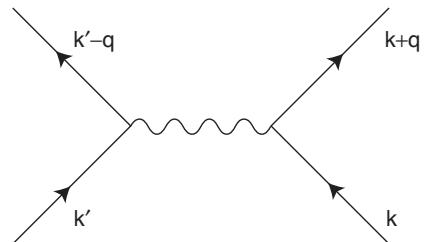
\includegraphics[width=0.55\textwidth]{figs/ch12/fig_12.8.jpg}
\caption*{图 12.8\quad 在费米面附近引起 BCS 配对的电子–声子相互作用。波浪线表示式 (12.35) 中的相互作用。}\label{fig:auto:12.8}
\end{figure}

\section{模型相互作用}

当然，在金属中我们还必须考虑电子–电子排斥。我们可以把这个势表示为
\begin{equation*}
V_{\mathrm{ee}}^{o}=\frac{V_{\mathrm{e}}(\mathbf{q})}{\varepsilon(\mathbf{q},\omega)},\tag{12.36}
\end{equation*}
其中 $\varepsilon(q,\omega)$ 是动态介电屏蔽函数。当然，电子–电子相互作用还有另一个来源，即由声子诱导的吸引。电子之间的完整相互作用具有如下形式
\begin{equation*}
V_{\mathrm{ee}}=\frac{V_{\mathrm{e}}(\mathbf{q})}{\varepsilon(\mathbf{q})}+\frac{\hbar\omega_{\mathbf{q}}\left|M_{\mathbf{q}}\right|^{2}}{\left(\Delta\epsilon_{\mathbf{k},\mathbf{q}}\right)^{2}-\left(\hbar\omega_{\mathbf{q}}\right)^{2}},\tag{12.37}
\end{equation*}
其中我们取了屏蔽函数的静态极限。现在 $\varepsilon(\mathbf{q})>0$，除非静态压缩率为负——如第9章所讨论的。这里我们排除这种情形，因为负压缩率出现在稀薄区间，那里需要对库仑相互作用作非微扰处理。通常，$V_{\mathrm{e}}(\mathbf{q})$ 远大于势的声子部分。然而，当 $\Delta\epsilon_{\mathbf{k},\mathbf{q}}\simeq\omega_{\mathbf{q}}$ 时，声子部分占主导，出现净吸引。于是我们看到，在不同的能量尺度上，声子部分或电子部分都可以占主导。相关的最大声子频率是 $\hbar\omega_{\mathrm{D}}$，即德拜能量。因此，当 $\Delta\epsilon_{\mathbf{k},\mathbf{q}}\le\hbar\omega_{\mathrm{D}}$ 时，产生的净吸引将压过电子排斥。当两个电子的能量都接近费米能量时，$\Delta\epsilon_{\mathbf{k},\mathbf{q}}\approx 0$，便得到吸引相互作用。这是 BCS 理论的一个本质特征。

在离开本节之前，考虑相互作用势 $V_{\mathrm{ee}}$ 的时间傅里叶变换是有益的。令 $\hbar\omega=\Delta\epsilon_{\mathbf{k},\mathbf{q}}$。$V_{\mathrm{ee}}$ 的傅里叶变换为
\begin{align*}
V_{\mathrm{ee}}(t)&=\int_{-\infty}^{\infty}\frac{\mathrm{d}\omega}{2\pi}\,\mathrm{e}^{-\mathrm{i}\omega t}\left[V_{\mathrm{ee}}^{o}+\frac{\hbar\omega_{\mathbf{q}}|M_{\mathbf{q}}|^{2}}{(\hbar\omega)^{2}-(\hbar\omega_{\mathbf{q}})^{2}}\right]\\
&=V_{\mathrm{ee}}^{o}\delta(t)+|M_{\mathbf{q}}|^{2}\frac{\hbar\omega_{\mathbf{q}}}{2\pi}\int_{-\infty}^{\infty}\frac{\mathrm{e}^{-\mathrm{i}\omega t}}{(\hbar\omega-\hbar\omega_{\mathbf{q}})(\hbar\omega+\hbar\omega_{\mathbf{q}})}\,\mathrm{d}\omega\\
&=V_{\mathrm{ee}}^{o}\delta(t)-|M_{\mathbf{q}}|^{2}\sin\omega_{\mathbf{q}}t.\tag{12.38}
\end{align*}

\begin{figure}[H]\centering
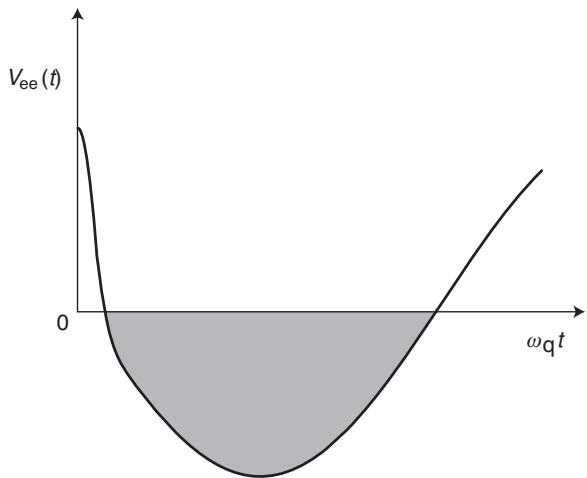
\includegraphics[width=0.6\textwidth]{figs/ch12/fig_12.9.jpg}
\caption*{图 12.9\quad 包含声子贡献的完整电子相互作用的傅里叶变换。电子排斥的 $\delta$ 函数贡献在 $t=0$ 附近被略微展宽。}\label{fig:auto:12.9}
\end{figure}

排斥部分只在 $t=0$ 起作用，而吸引部分是时间的振荡函数。总势示于图12.9。我们发现，电子势只在声子吸引占主导的那段时间间隔内是吸引的。这是关键的一点：时域中的 $V_{\mathrm{ee}}$ 并不总是吸引的。电子排斥与声子介导的吸引作用在不同的时间尺度上，因此电子的配对束缚是可能的。

让我们计算两体散射幅
\begin{equation*}
A_{\mathrm{s}}=\left\langle\mathbf{p}_{4\sigma_{1}}\mathbf{p}_{3\sigma_{2}}\right|V_{\mathrm{ee}}\left|\mathbf{p}_{1\sigma_{1}}\mathbf{p}_{2\sigma_{2}}\right\rangle,\tag{12.39}
\end{equation*}
其中
\begin{equation*}
V_{\mathrm{ee}}=\sum_{\mathbf{k},\mathbf{k}',\mathbf{q}}V(\mathbf{k},\mathbf{k}'-\mathbf{q})a_{\mathbf{k}+\mathbf{q}}^{\dagger}a_{\mathbf{k}'-\mathbf{q}}^{\dagger}a_{\mathbf{k}'}a_{\mathbf{k}}.\tag{12.40}
\end{equation*}
如第5章所讨论的，任何这种形式的两体幅都分解为直接与交换库仑积分之差。对一般的依赖动量的势，直接项与交换项将以动量和自旋的不同组合进入。例如，交换项将具有 $V(\mathbf{p}_{1},\mathbf{p}_{3})$ 的形式且 $\sigma_{1}=\sigma_{2}$，而直接项进入时对自旋没有限制，且依赖于 $V(\mathbf{p}_{1},\mathbf{p}_{4})$。让我们假定净吸引势是一个形如下式的常数
\begin{equation*}
V_{\mathrm{ee}}=\begin{cases}-V_{o}, & \left|\Delta\epsilon_{\mathbf{k}_{\mathrm{F}},\mathbf{q}}\right|<\hbar\omega_{\mathrm{D}},\\ 0, & \left|\Delta\epsilon_{\mathbf{k}_{\mathrm{F}},\mathbf{q}}\right|>\hbar\omega_{\mathrm{D}}.\end{cases}\tag{12.41}
\end{equation*}
由于势与动量无关，直接积分与交换积分相等，且当 $\sigma_{1}=\sigma_{2}$ 时散射幅为零。唯一非零的贡献来自 $\sigma_{1}\neq\sigma_{2}$。因此，对常数相互作用，只有当电子被锁定成单态时散射幅才非零。在这种情形下，声子在自旋相反的电子之间诱导出净吸引。相应的矩阵元形式为
\begin{equation*}
\left\langle\mathbf{p}_{4\uparrow}\mathbf{p}_{3\downarrow}\right|V_{\mathrm{ee}}\left|\mathbf{p}_{1\uparrow}\mathbf{p}_{2\downarrow}\right\rangle=-V_{0}\delta_{\mathbf{p}_{1}+\mathbf{p}_{2},\,\mathbf{p}_{3}+\mathbf{p}_{4}}\tag{12.42}
\end{equation*}
适用于费米面附近的散射。锁定成单态的两个粒子将在费米能级处产生能隙。

\section{库珀对}

现在考虑一个多少有些人为的问题：一个包含 $N$ 个无相互作用电子的满费米海，另有两个相互作用的电子处于海外。由于泡利不相容原理，费米海之外的电子其动量必须超过 $p_{\mathrm{F}}$。我们取相互作用势为上一节导出的常数单态对势，即式 (12.42)。于是自旋波函数对自旋是反对称的。相应的空间部分必须是对称的，以满足总体反对称性要求。我们这个两粒子子系统的本征值方程为
\begin{equation*}
\left[-\frac{\hbar^{2}}{2m}\bigl(\nabla_{1}^{2}+\nabla_{2}^{2}\bigr)+V(\mathbf{r}_{1}-\mathbf{r}_{2})-E\right]\Psi(\mathbf{r}_{1},\mathbf{r}_{2};\uparrow_{1},\downarrow_{2})=0.\tag{12.43}
\end{equation*}
一般地，两体波函数是一个复合态
\begin{equation*}
\Psi(\mathbf{r}_{1},\mathbf{r}_{2};\uparrow_{1},\downarrow_{2})=\psi(\mathbf{r}_{1},\mathbf{r}_{2})\chi_{S}(\uparrow_{1},\downarrow_{2}),\tag{12.44}
\end{equation*}
其中 $\chi_{S}(\uparrow_{1},\downarrow_{2})$ 表示单态自旋态，而 $\psi$ 包含空间依赖性。对两个粒子，我们可以用相对坐标 $\mathbf{r}=\mathbf{r}_{1}-\mathbf{r}_{2}$ 与质心 $\mathbf{R}=(\mathbf{r}_{1}+\mathbf{r}_{2})/2$ 把空间波函数表达为
\begin{equation*}
\psi(\mathbf{r}_{1},\mathbf{r}_{2})=\varphi(\mathbf{r})\,\mathrm{e}^{\mathrm{i}\mathbf{Q}\cdot\mathbf{R}/\hbar}.\tag{12.45}
\end{equation*}
同样，我们感兴趣的动量是质心动量 $\mathbf{Q}=\mathbf{p}_{1}+\mathbf{p}_{2}$ 与相对动量 $\mathbf{q}=(\mathbf{p}_{1}-\mathbf{p}_{2})/2$。我们把 $\varphi(\mathbf{r})$ 展开为傅里叶级数
\begin{equation*}
\varphi(\mathbf{r})=\sum_{\mathbf{k}}^{\prime}\frac{\mathrm{e}^{\mathrm{i}\mathbf{k}\cdot\mathbf{r}/\hbar}}{\sqrt{V}}\,\alpha_{\mathbf{k}},\tag{12.46}
\end{equation*}
其中撇号表示求和限于 $\mathbf{k}>\mathbf{k}_{\mathrm{F}}$，即所有能量超过 $\epsilon_{\mathrm{F}}$ 的态。由于 $\mathbf{k}\cdot\mathbf{r}=\mathbf{k}\cdot\mathbf{r}_{1}-\mathbf{k}\cdot\mathbf{r}_{2}$，我们看到对态具有动量 $(\mathbf{k},-\mathbf{k})$。注意，若 $\mathbf{k}_{1}+\mathbf{k}_{2}=0$，则质心运动从问题中消失。

我们首先关注 $\mathbf{Q}=0$ 的解。为此，我们定义相互作用势的傅里叶分量
\begin{equation*}
V_{\mathbf{k}\mathbf{k}'}=\int\frac{\mathrm{d}\mathbf{r}}{V}\,\mathrm{e}^{-\mathrm{i}(\mathbf{k}-\mathbf{k}')\cdot\mathbf{r}/\hbar}V(\mathbf{r}),\tag{12.47}
\end{equation*}
并引入质心薛定谔方程
\begin{equation*}
\left(-\frac{\hbar^{2}}{2\mu}\nabla^{2}+V(\mathbf{r})\right)\varphi(\mathbf{r})=E\varphi(\mathbf{r}),\tag{12.48}
\end{equation*}
其中 $\mu$ 是约化质量，$\mu=m/2$。代入 $\varphi(\mathbf{r})$ 的傅里叶表示，乘以 $\exp(-\mathrm{i}\mathbf{k}\cdot\mathbf{r}/\hbar)$ 并积分，我们得到
\begin{equation*}
\left(E-2\epsilon_{\mathbf{k}}\right)\alpha_{\mathbf{k}}=\sum_{\mathbf{k}'}V_{\mathbf{k}\mathbf{k}'}\alpha_{\mathbf{k}'}\tag{12.49}
\end{equation*}
作为我们的新本征值方程。这里 $\epsilon_{\mathbf{k}}=k^{2}/2m$。矩阵元 $V_{\mathbf{k}\mathbf{k}'}$ 等价于
\begin{equation*}
V_{\mathbf{k}\mathbf{k}'}=\left\langle\mathbf{k},-\mathbf{k}\right|V_{\mathrm{ee}}\left|\mathbf{k}',-\mathbf{k}'\right\rangle.\tag{12.50}
\end{equation*}
$V_{\mathbf{k}\mathbf{k}'}$ 中一个典型的散射过程示于图12.10。

\begin{figure}[H]\centering
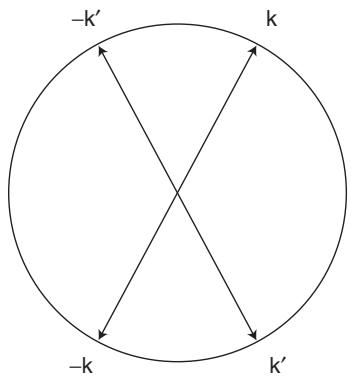
\includegraphics[width=0.5\textwidth]{figs/ch12/fig_12.10.jpg}
\caption*{图 12.10\quad 跨越费米面的一对电子态之间的散射。}\label{fig:auto:12.10}
\end{figure}

如果现在引入近似
\begin{equation*}
V_{\mathbf{k}\mathbf{k}'}=\begin{cases}-V_{0}, & k,k'>p_{\mathrm{F}},\\ 0, & \text{其余情形},\end{cases}\tag{12.51}
\end{equation*}
则本征值方程可以改写为
\begin{align*}
1&=-V_{0}\sum_{k>k_{\mathrm{F}}}\frac{1}{E-2\epsilon_{\mathbf{k}}}\\
&=-V_{0}\phi(E).\tag{12.52}
\end{align*}
只要 $\phi(E)=-1/V_{0}$，此方程即被满足。$\phi(E)$ 的极点位于 $E=2\epsilon_{\mathbf{k}}$，即该对的总能量，其下界为 $2\epsilon_{\mathrm{F}}$。在有限系统中，由于 $\mathbf{k}$ 是量子化的，$\epsilon_{\mathbf{k}}$ 取分立值。当 $E$ 从下方趋近 $2\epsilon_{\mathbf{k}}$ 时，$\phi(E)$ 趋于 $-\infty$；恰在 $2\epsilon_{\mathbf{k}}$ 上方，$\phi(E)$ 约为 $+\infty$。对所有 $E<2\epsilon_{\mathrm{F}}$，$\phi(E)$ 为负。因此，当 $\phi(E)$ 在 $E<2\epsilon_{\mathrm{F}}$ 处穿过 $-1/V_{0}$ 时，一个束缚态便形成了。$-1/V_{0}$ 与 $\phi(E)$ 的交点在图12.11中以图解方式给出。这种解的存在性就是库珀（Cooper）对问题（文献 [C1956]）。

\begin{figure}[H]\centering
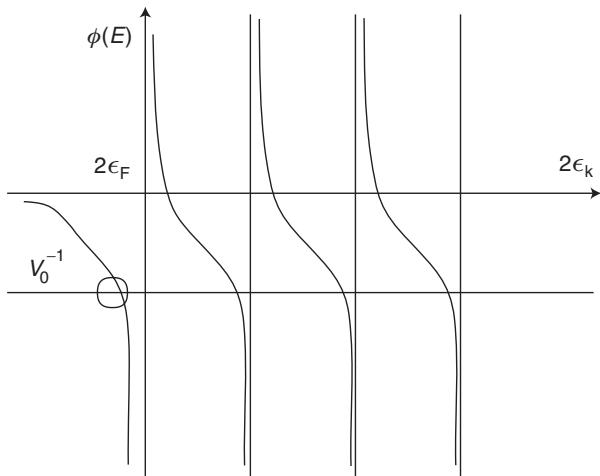
\includegraphics[width=0.62\textwidth]{figs/ch12/fig_12.11.jpg}
\caption*{图 12.11\quad 库珀对问题中 $\phi(E)$ 对 $\epsilon_{\mathbf{k}}$ 的图像。$\phi(E)$ 与直线 $-V_{0}^{-1}$ 的交点确定该对的束缚态解。}\label{fig:auto:12.11}
\end{figure}

为求出束缚态的精确能量，我们把式 (12.52) 中的求和换成积分，
\begin{equation*}
1=V_{0}\sum_{\epsilon(\mathbf{k})}^{\prime}\frac{1}{2\epsilon_{\mathbf{k}}-E}\ \to\ V_{0}\int_{\epsilon_{\mathrm{F}}}^{\epsilon_{\mathrm{F}}+\hbar\omega_{\mathrm{D}}}\frac{N(x)\,\mathrm{d}x}{2x-E}\tag{12.53}
\end{equation*}
其中引入了态密度 $N(x)$。若假定 $N(x)$ 在窄的积分区间内变化不大，则可取 $N(x)\approx N(\epsilon_{\mathrm{F}})$。在这些假设下，积分给出
\begin{equation*}
-\frac{2}{V_{0}N(\epsilon_{\mathrm{F}})}=\ln\left[\frac{\epsilon_{\mathrm{F}}-\frac{E}{2}}{\epsilon_{\mathrm{F}}-\frac{E}{2}+\hbar\omega_{\mathrm{D}}}\right],\tag{12.54}
\end{equation*}
由此可得
\begin{equation*}
\left(\epsilon_{\mathrm{F}}-\frac{E}{2}+\hbar\omega_{\mathrm{D}}\right)\exp\left(-\frac{2}{V_{0}N(\epsilon_{\mathrm{F}})}\right)=\epsilon_{\mathrm{F}}-\frac{E}{2}.\tag{12.55}
\end{equation*}
这个线性方程可以立即解出本征能量 $E$：
\begin{equation*}
E=2\epsilon_{\mathrm{F}}-\frac{2\hbar\omega_{\mathrm{D}}\exp\left(-2/V_{0}N(\epsilon_{\mathrm{F}})\right)}{1-\exp\left(-2/V_{0}N(\epsilon_{\mathrm{F}})\right)}.\tag{12.56}
\end{equation*}
在 $2\gg V_{0}N(\epsilon_{\mathrm{F}})$ 的极限下，分母中的指数函数可以展开。弱耦合极限下的对束缚能
\begin{equation*}
E\simeq 2\epsilon_{\mathrm{F}}-2\hbar\omega_{\mathrm{D}}\exp\left(-\frac{2}{V_{0}N(\epsilon_{\mathrm{F}})}\right)\tag{12.57}
\end{equation*}
随之得出。这两个表达式中的任何一个都表明：只要 $V_{0}$ 非零且为正，库珀对就以低于 $2\epsilon_{\mathrm{F}}$ 的能量束缚。这是一个深刻的结果。它意味着，只要存在式 (12.51) 形式的吸引相互作用，费米面正下方的两个电子可以通过被激发成动量为 $(\mathbf{k},-\mathbf{k})$、恰在费米面之上的库珀对而降低其能量。这就是所谓的库珀失稳（Cooper instability）。

进一步，我们可以估计对束缚能如何依赖于库珀对的质心。一开始我们猜想这个量可能按 $Q^{2}$ 标度。我们将证明并非如此。为推进讨论，我们把对束缚判据推广到 $Q\neq 0$ 的情形。对非零的 $Q$，该对的裸能量变为 $\epsilon_{\mathbf{q}+\mathbf{Q}/2}+\epsilon_{-\mathbf{q}+\mathbf{Q}/2}$。于是，对束缚条件变为
\begin{equation*}
1=-V_{0}\sum_{\mathbf{q}}\frac{1}{E-\epsilon_{\mathbf{q}+\mathbf{Q}/2}-\epsilon_{-\mathbf{q}+\mathbf{Q}/2}}.\tag{12.58}
\end{equation*}
对小的 $Q$，在略去 $O(Q^{2})$ 的项后，我们可以把式 (12.58) 改写为
\begin{equation*}
1=-V_{0}\int_{\epsilon_{\mathrm{F}}+v_{\mathrm{F}}Q/2}^{\epsilon_{\mathrm{F}}+v_{\mathrm{F}}Q/2+\hbar\omega_{\mathrm{D}}}\frac{N(\epsilon_{\mathbf{q}})\,\mathrm{d}\epsilon_{\mathbf{q}}}{E-2\epsilon_{\mathbf{q}}},\tag{12.59}
\end{equation*}
质心只不过移动了费米能量的零点。新的对束缚能
\begin{equation*}
E=2\epsilon_{\mathrm{F}}+Qv_{\mathrm{F}}-\frac{2\hbar\omega_{\mathrm{D}}}{\exp\left(2/V_{0}N(\epsilon_{\mathrm{F}})\right)-1},\tag{12.60}
\end{equation*}
是质心动量的线性函数。质心的平移会强烈地降低束缚能，最终可能拆散这个对。为说明这一点，我们令 $\epsilon_{\mathrm{F}}=0$，求出库珀对损失其大部分束缚能时的 $Q$ 值。我们必须求解
\begin{align*}
Qv_{\mathrm{F}}&=\frac{2\hbar\omega_{\mathrm{D}}}{\exp\left(2/V_{0}N(\epsilon_{\mathrm{F}})\right)-1}\\
&\approx k_{\mathrm{B}}T_{\mathrm{c}}.\tag{12.61}
\end{align*}
等价地，$Q/\hbar\sim k_{\mathrm{B}}T_{\mathrm{c}}/\hbar v_{\mathrm{F}}\sim 10^{4}\,\mathrm{cm}^{-1}$，大致是皮帕德（Pippard）相干长度 $\xi\sim 10^{-4}\,\mathrm{cm}$ 的倒数。这是库珀对的有效回转半径，与原子间距相比是一个巨大的距离。如此大的相干长度是声子配对机制的典型特征。

\section{费米液体理论}

当然，我们的问题在某种程度上是人为的，因为我们忽略了除恰在费米面上方的那一对电子以外的所有电子间相互作用。一旦考虑全体电子之间的排斥相互作用，库珀失稳的简单图像理应失效，这是完全合理的预期。也就是说，当电子彼此相互作用时，我们不能先验地把无相互作用的本征态当作系统的有效描述（正如我们在库珀问题中所做的那样）。于是我们面临这样的问题：这种失稳是真实的吗？我们将从两条途径回答这一问题：一是借助费米面附近电子散射的简单物理考虑，二是借助对完整相互作用拉格朗日量作标度分析的更形式化的论证。如今人们普遍接受：金属的正常态由朗道–费米液体理论描述。按照这一理论，电子间相互作用在金属中的主导效应是重正化电子的有效质量，观测到的移动约为 10\% 到 50\% 的量级。费米液体理论的另一条本质论断是：金属正常态的激发态与无相互作用电子气的激发态之间存在一一对应。费米液体理论中的元激发称为准粒子（quasi-particle）。准粒子是一种具有寿命的复合粒子，其寿命源于与其他准粒子的碰撞。当准粒子的寿命 $\tau$ 为无穷大时，含这种粒子的态就是系统的本征态。然而，准粒子态要成为系统的本征态所必须满足的最低约束是 $\hbar/\tau\ll\tilde{\epsilon}_{\mathbf p}$，其中 $\tilde{\epsilon}_{\mathbf p}$ 是准粒子的能量。我们将在下文看到，当准粒子的能量趋近费米能级时，其寿命趋于无穷。准粒子在费米能级处的稳定性是费米液体理论的一条关键信条。

费米能级附近电子散射率趋于零可以证明如下。考虑一个接近 $T=0$ 的分布，其中除一个电子外所有电子都处于费米面以下。设 $\epsilon_1$ 为费米面之上那个电子的能量。具有该能量的电子要散射，必须与某个能量为 $\epsilon_2<\epsilon_{\mathrm F}$ 的电子相互作用。泡利不相容原理要求散射事件之后两个电子必须占据费米面以上的两个态。设这两个态的能量为 $\epsilon_3$ 与 $\epsilon_4$。能量守恒要求 $\epsilon_1+\epsilon_2=\epsilon_3+\epsilon_4$。若 $\epsilon_1=\epsilon_{\mathrm F}$，则为满足能量守恒，其余所有态也必须处于费米能级。因此，对处于费米能级的电子，可被散射进去的态数为零。于是，正比于散射态密度的散射率必定为零。结果是费米能级处电子或准粒子的寿命为无穷大。

\begin{figure}[H]\centering
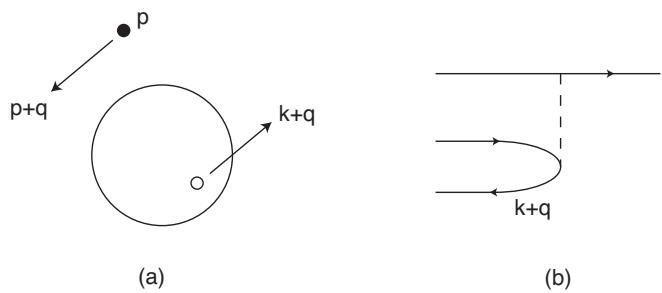
\includegraphics[width=0.62\textwidth]{figs/ch12/fig_12.12.jpg}
\caption*{图 12.12\quad（a）一个受激准粒子与基态中粒子的散射。（b）动量空间散射的图示表示。}\label{fig:auto:12.12}
\end{figure}

当 $\epsilon_1$ 离开费米能级时，存在一个宽度为 $\epsilon_1-\epsilon_{\mathrm F}$ 的态窗口，其余三个电子态可以从中选取。一旦从这个宽为 $\epsilon_1-\epsilon_{\mathrm F}$ 的窄窗中选定了其中两个态，由于能量守恒，最后一个态的能量便不能自由选取。因此，$\epsilon_2$ 有 $\epsilon_1-\epsilon_{\mathrm F}$ 种选择，$\epsilon_3$ 有 $\epsilon_1-\epsilon_{\mathrm F}$ 种选择，而 $\epsilon_4$ 随之确定。结果，散射率应当按 $(\epsilon_1-\epsilon_{\mathrm F})^2$ 标度。

为了更严格地看到这一点，我们计算动量态 $-\mathbf k$ 与 $-\mathbf k-\mathbf q$ 上的两个粒子散射到态 $\mathbf p$ 与 $\mathbf p+\mathbf q$ 的散射率。这一相互作用描绘于图 12.12。该过程的散射率为
\begin{equation*}
\frac{1}{\tau}=\frac{2\pi}{\hbar}\sum_{\mathbf q,\mathbf k,\sigma}|V(q)|^2 n_{\mathbf k\sigma}\left(1-n_{\mathbf k-\mathbf q\,\sigma}\right)\left(1-n_{\mathbf p+\mathbf q}\right)\delta\left(\hbar\omega_{\mathbf p\mathbf q}+\hbar\omega_{\mathbf k\mathbf q}\right), \tag{12.62}
\end{equation*}
其中 $V(q)$ 是库仑势的傅里叶变换，而 $\hbar\omega_{\mathbf p\mathbf q}=\epsilon_{\mathbf p+\mathbf q}-\epsilon_{\mathbf p}$。由能量守恒可得 $|\mathbf p+\mathbf q|<p$ 且 $|\mathbf p+\mathbf q|>p_{\mathrm F}$。这些条件概括为约束 $p_{\mathrm F}^2<|\mathbf p+\mathbf q|^2<p^2$，或者等价地
\begin{equation*}
p_{\mathrm F}^2-p^2<2pq\cos\theta+q^2<0. \tag{12.63}
\end{equation*}
正如我们在分析屏蔽时那样，可以利用自由粒子屏蔽函数的定义（见式 (9.103)）来简化对 $\mathbf k$ 的求和。在 $T=0$ 下，我们得到
\begin{equation*}
\frac{1}{\tau}=\frac{n_e}{2\hbar^2}\sum_{\mathbf q}|V(q)|^2 S_0(q,\hbar\omega_{\mathbf p\mathbf q})\left(1-n_{\mathbf p+\mathbf q}\right). \tag{12.64}
\end{equation*}
因为我们主要关注 $p-p_{\mathrm F}\approx 0$，故可取 $q$ 为小量。于是我们在托马斯–费米近似下取屏蔽库仑势的 $q\to 0$ 极限，$V(q\to 0)=4\pi e^2/V\kappa_{\mathrm{TF}}^2$。同时，取第 9 章导出的结构函数的 $q\to 0$ 形式：
\begin{equation*}
S(q,\omega_{\mathbf p\mathbf q})\propto\frac{\omega_{\mathbf p\mathbf q}}{q}. \tag{12.65}
\end{equation*}
因此，散射率简化为
\begin{equation*}
\frac{1}{\tau}\propto\frac{1}{\epsilon_{\mathrm F}}\int\sin\theta\,\mathrm d\theta\int q\,\omega_{\mathbf p\mathbf q}\,\mathrm d q. \tag{12.66}
\end{equation*}
通过求解 $\hbar\omega_{\mathbf p\mathbf q}=(2pq\cos\theta+q^2)/2m$，我们可以把对 $q$ 的积分换成对 $\omega_{\mathbf p\mathbf q}$ 的积分。散射率正比于
\begin{align*}
\frac{1}{\tau}&\propto\frac{1}{\epsilon_{\mathrm F}}\int_0^{\epsilon_{\mathrm p}-\epsilon_{\mathrm F}}\mathrm d\omega\int_{-1}^{1}\omega\left(1-\frac{xp_{\mathrm F}}{\sqrt{x^2p_{\mathrm F}^2+\omega}}\right)\mathrm d x\\
&\propto\frac{1}{\epsilon_{\mathrm F}}\int_0^{\epsilon_{\mathrm p}-\epsilon_{\mathrm F}}\omega\,\mathrm d\omega\propto\frac{(\epsilon_{\mathrm p}-\epsilon_{\mathrm F})^2}{\epsilon_{\mathrm F}}. \tag{12.67}
\end{align*}
于是我们清楚地看到，散射率按 $(\epsilon_{\mathbf p}-\epsilon_{\mathrm F})^2$ 标度，因而在费米能级处的态上为零。取 $\epsilon_{\mathbf p}-\epsilon_{\mathrm F}\propto k_{\mathrm B}T$，我们发现散射率正比于 $T^2$。正如上一章所述，铜氧化物高温 $T_{\mathrm c}$ 材料正常态的电阻率 [GF1987] 在直到 $T_{\mathrm c}$ 的温区内随温度线性变化。对照费米液体的结果，这种行为强烈暗示这些材料的正常态是非费米液体。

准粒子散射率对温度的二次依赖是费米液体理论的一个核心预言。室温下 $(k_{\mathrm B}T)^2/\epsilon_{\mathrm F}$ 的量级为 $10^{-4}\,\mathrm{eV}$。由此给出的散射寿命在室温下为 $10^{-10}\,\mathrm{s}$ 的量级。金属中典型的弛豫时间比这短四个数量级（见第 11 章）。因此，电子–电子相互作用并不是费米能级附近电子的主导散射机制。正因如此，无相互作用的图像才如此有效，是金属正常态性质的良好近似——至少在室温下如此。当然，在足够低的温度下，电子–电子相互作用的重要性急剧增大，超导电性就是一个现成的例子。

费米液体理论的终极表述 [P1992; SM1991; BG1990] 是：短程排斥相互作用在费米面处是无关的（irrelevant）。一旦我们建立起关于费米子相干态的若干预备结果，这一表述便可以从相互作用系统的拉格朗日量的标度分析中得到证明。费米子相干态与费米子算符 $\Psi$ 由本征值方程
\begin{equation*}
\Psi|\psi\rangle=\psi|\psi\rangle, \tag{12.68}
\end{equation*}
相联系，其中 $|\psi\rangle$ 是费米子相干态。然而，本征值 $\psi$ 并非普通的数。它的平方 $\psi^2$ 为零，从而蕴含如下一系列等式
\begin{equation*}
\Psi^2|\psi\rangle=\psi^2|\psi\rangle=0|\psi\rangle \tag{12.69}
\end{equation*}
成立。$\psi$ 是一个格拉斯曼（Grassmann）变量，即一个反对易的数。虽然这看似古怪，但格拉斯曼数的平方为零恰恰是我们在费米子路径积分表述中把泡利原理纳入其中的所需之物。

那么，使式 (12.68) 成为可能的态 $|\psi\rangle$ 究竟是什么？我们作如下拟设（ansatz）
\begin{equation*}
|\psi\rangle=|0\rangle-\psi|1\rangle \tag{12.70}
\end{equation*}
它符合费米子相干态的要求。这里 $\Psi|0\rangle=0=\Psi^\dagger|1\rangle=0$ 且 $\Psi|1\rangle=|0\rangle$。我们按如下方式检验该拟设，首先注意
\begin{equation*}
\Psi|\psi\rangle=-\Psi\psi|1\rangle=\psi\Psi|1\rangle=\psi|0\rangle. \tag{12.71}
\end{equation*}
然而 $|0\rangle=|\psi\rangle+\psi|1\rangle$。代入后得到
\begin{equation*}
\Psi|\psi\rangle=\Psi\left[|\psi\rangle+\psi|1\rangle\right]=\psi|\psi\rangle, \tag{12.72}
\end{equation*}
此即所求。因此 $|\psi\rangle$ 构成一个费米子相干态。现在考虑伴随 $\langle\bar\psi|\Psi^\dagger$。量子力学的标准规则可以应用于伴随。例如
\begin{equation*}
\langle\bar\psi|\Psi^\dagger\equiv\langle\bar\psi|\bar\psi. \tag{12.73}
\end{equation*}
利用 $\bar\psi\langle 1|=-\langle 1|\bar\psi$ 这一事实，我们得到
\begin{align*}
\langle\bar\psi|\psi\rangle&=\langle 0|0\rangle+\bar\psi\psi\langle 1|1\rangle\\
&=1+\bar\psi\psi=\mathrm e^{\bar\psi\psi}. \tag{12.74}
\end{align*}
这个表达式可能显得有些奇怪，因为截断绝非源于 $\bar\psi\psi$ 的小。这个量既不大也不小。截断之所以成立，是因为格拉斯曼变量的平方为零。

继续往下，我们需要几个积分：
\begin{equation*}
\int\psi\,\mathrm d\psi=1, \tag{12.75}
\end{equation*}
\begin{equation*}
\int\mathrm d\psi=\int\mathrm d\bar\psi=0, \tag{12.76}
\end{equation*}
\begin{equation*}
\int\bar\psi\psi\,\mathrm d\bar\psi\,\mathrm d\psi=-1, \tag{12.77}
\end{equation*}
\begin{equation*}
\int\mathrm e^{-a\bar\psi\psi}\mathrm d\bar\psi\,\mathrm d\psi=\int\left(1-a\bar\psi\psi\right)\mathrm d\bar\psi\,\mathrm d\psi=a, \tag{12.78}
\end{equation*}
\begin{equation*}
\int\mathrm e^{-\bar\psi M\psi}\mathrm d\bar\psi\,\mathrm d\psi=\mathrm{Det}\,M. \tag{12.79}
\end{equation*}
这些积分使我们能够建立若干恒等式。首先是恒等算符的分解，
\begin{equation*}
\int|\psi\rangle\langle\bar\psi|\mathrm e^{-\bar\psi\psi}\mathrm d\bar\psi\,\mathrm d\psi=|0\rangle\langle 0|+|1\rangle\langle 1|=I, \tag{12.80}
\end{equation*}
它在费米子相干态的表述下具有格外简单的形式。在用费米子相干态写出路径积分时，我们还需要玻色型算符的迹的表达式。所谓玻色型，我们只是指由偶数个费米子算符构成的算符。考虑量
\begin{align*}
\langle-\bar\psi|\psi\rangle&=\left[\langle 0|-\bar\psi\langle 1|\right]\left[|0\rangle-\psi|1\rangle\right]\\
&=\langle 0|0\rangle-\bar\psi\psi\langle 1|1\rangle. \tag{12.81}
\end{align*}
为得到对角元之和，我们计算积分
\begin{equation*}
\int\left[\langle 0|0\rangle-\bar\psi\psi\langle 1|1\rangle\right]\mathrm e^{-\bar\psi\psi}\mathrm d\bar\psi\,\mathrm d\psi=\langle 0|0\rangle+\langle 1|1\rangle. \tag{12.82}
\end{equation*}
因此，迹公式为
\begin{equation*}
\mathrm{Tr}\,\Omega=\int\langle-\bar\psi|\Omega|\psi\rangle\mathrm e^{-\bar\psi\psi}\mathrm d\bar\psi\,\mathrm d\psi. \tag{12.83}
\end{equation*}

利用这些关系，我们来表达配分函数
\begin{equation*}
Z=\mathrm{Tr}\,\mathrm e^{-\beta H}, \tag{12.84}
\end{equation*}
把它写成相干态的形式。通过与标准薛定谔传播子的类比，我们把 $\beta$ 确认为一个虚时间。我们用 $\epsilon=\beta/N$ 对这个“时间”区间作细分，并把玻尔兹曼权重
\begin{equation*}
Z=\lim_{N\to\infty}\mathrm{Tr}\left[\mathrm e^{-\epsilon H}\right]^N \tag{12.85}
\end{equation*}
提升到 $N$ 次幂。在大 $N$ 极限下，我们可以把指数因子截断到第一项。为紧凑起见，我们定义 $\hat D_\epsilon\equiv\hat D_\epsilon(\psi^\dagger,\psi)=1-\epsilon H$。然后利用谱分解的单位元，即式 (12.80)，得到
\begin{align*}
Z=\int{}&\langle-\bar\psi_0|\hat D_\epsilon|\psi_{N-1}\rangle\mathrm e^{-\bar\psi_{N-1}\psi_{N-1}}\langle\bar\psi_{N-1}|\hat D_\epsilon|\psi_{N-2}\rangle\mathrm e^{\bar\psi_{N-2}\psi_{N-2}}\\
&\times\langle\bar\psi_{N-2}|\cdots|\psi_1\rangle\mathrm e^{-\bar\psi_1\psi_1}\langle\bar\psi_1|\hat D_\epsilon|\psi_0\rangle\mathrm e^{-\bar\psi_0\psi_0}\prod_{i=0}^{N-1}\mathrm d\bar\psi_i\,\mathrm d\psi_i \tag{12.86}
\end{align*}
作为配分函数的工作表达式。假定 $H$ 中所有算符都是正规序的，使得 $H|0\rangle=0$。于是
\begin{equation*}
\langle\bar\psi_{i+1}|\hat D_\epsilon|\psi_i\rangle=\langle\bar\psi_{i+1}|D_\epsilon(\psi^\dagger_{i+1},\psi_i)|\psi_i\rangle=\mathrm e^{\bar\psi_{i+1}\psi_i}\mathrm e^{-\epsilon H(\psi^\dagger_{i+1},\psi_i)}. \tag{12.87}
\end{equation*}
大功告成在即。我们只需把式 (12.87) 代入式 (12.86) 共 $N$ 次，
\begin{equation*}
Z=\lim_{N\to\infty}\int\prod_{i=0}^{N-1}\mathrm e^{\left[\left(\frac{(\bar\psi_{i+1}-\bar\psi_i)}{\epsilon}\psi_i-H\right)\epsilon\right]}\mathrm d\bar\psi_i\,\mathrm d\psi_i, \tag{12.88}
\end{equation*}
其中我们定义了 $\bar\psi_N=-\bar\psi_0$ 与 $\psi_N=-\psi_0$，且 $\psi_N$ 与 $\bar\psi_N$ 明确不参与积分。在 $N\to\infty$ 极限下，可以把指数中的求和化为积分。对时间导数项分部积分并利用边界条件 $\psi(0)=\psi(\beta)=0$，我们把配分函数化为标准形式
\begin{equation*}
Z=\int\mathcal D\bar\psi\,\mathcal D\psi\,\mathrm e^{-S_{\mathrm E}}, \tag{12.89}
\end{equation*}
其中 $S_{\mathrm E}$
\begin{equation*}
S_{\mathrm E}=\int\left(\bar\psi\partial_\tau\psi+H\right)\mathrm d^d x\,\mathrm d\tau, \tag{12.90}
\end{equation*}
是欧几里得作用量，$\tau$ 的积分在区间 $[0,\beta]$ 上进行。这是一切费米子量子场论的出发点。

考虑无相互作用电子的情形。哈密顿量
\begin{equation*}
H=\sum_{\mathbf p,\sigma}\left(\epsilon_{\mathbf p}-\epsilon_{\mathrm F}\right)\psi^\dagger_\sigma(\mathbf p)\psi_\sigma(\mathbf p), \tag{12.91}
\end{equation*}
用动量空间的产生与湮灭算符写出十分方便，其中 $\epsilon(\mathbf p)$ 是自由粒子色散关系，$\epsilon_{\mathrm F}$ 是费米能。相应的作用量为
\begin{equation*}
S=\int\mathrm d t\,\mathrm d^3\mathbf p\left(\mathrm i\psi^\dagger_\sigma(\mathbf p)\partial_t\psi_\sigma(\mathbf p)-\psi^\dagger_\sigma(\mathbf p)\left(\epsilon_{\mathbf p}-\epsilon_{\mathrm F}\right)\psi_\sigma(\mathbf p)\right), \tag{12.92}
\end{equation*}
这里我们已经换到实时间。严格说来，作用量应当用费米子相干态而不是费米子产生、湮灭算符来写。虽然这一区别对我们这里考虑的应用并不关键，但在费米子路径积分中使用费米子相干态却是至关重要的。尽管如此，约定俗成的是：用产生、湮灭算符写出的路径积分实际上暗含以相干态为工作基。

我们希望考虑朝向费米面的标度变换。首先需要引入标度维数的概念。考虑简单函数 $f(x)=x^2$。在标度 $x\to sx$ 下，$f(x)\to s^2x^2$，其中假定 $s$ 为正。若 $s\to 0$，函数 $f$ 随之消失。我们把参数 $x$ 的标度维数定义为：为得到 $x$ 的标度变换，标度因子 $s$ 必须被提升到的幂次。操作上，
\begin{equation*}
\mathrm{Dim}[x]=\frac{\mathrm d f}{\mathrm d s}\frac{s}{f}=\frac{\mathrm d\ln f}{\mathrm d\ln s}=2. \tag{12.93}
\end{equation*}
在场论的语境下，标度维数起着基本作用。让我们把作用量分割为
\begin{equation*}
S=S_0+S_{\mathrm{int}}, \tag{12.94}
\end{equation*}
其中所有相互作用都包含在
\begin{equation*}
S_{\mathrm{int}}=\int\mathrm d t\,\mathrm d^d\mathbf k\,\mathcal O(\mathbf k,t) \tag{12.95}
\end{equation*}
之中。这里 $\mathcal O$ 是某个算符（当然是由基本场构成的复合算符），它决定相互作用。我们这样选取时间、动量和裸场的标度，使得 $S_0\to s^0S_0=S_0$。在这种标度选取下，相互作用项将变换为 $s^bS_{\mathrm{int}}$。若 $b>0$，则由 $\mathcal O$ 生成的相互作用是无关的，因为它们在标度极限下消失；此时我们称 $\mathcal O$ 为无关算符。若 $b<0$，则 $\mathcal O$ 是相关的。$b=0$ 时出现边际（marginal）情形。由于我们考虑的是朝向费米面的标度，我们希望这样标度所有的场与空间、时间坐标，使相关的自由粒子作用量的标度维数为零。随后我们将证明：把同样的标度用于任何排斥性短程四费米子相互作用时，只要 $d\ge 2$，其标度维数必为正。跟随波尔钦斯基（Polchinski）[P1992]，我们把一个电子的动量写作
\begin{equation*}
\mathbf p=\mathbf k+\boldsymbol\ell, \tag{12.96}
\end{equation*}
即两个动量之和：一个位于费米面上（$\mathbf k$），另一个垂直于它（$\boldsymbol\ell$），后者代表对费米面的偏离。于是，我们在费米面附近展开电子的色散关系
\begin{equation*}
\epsilon(\mathbf p)=\epsilon_{\mathrm F}+\ell\frac{\partial\epsilon}{\partial\mathbf p}+O(\ell^2), \tag{12.97}
\end{equation*}
只保留线性项。由于能量零点取在费米面上，保持费米面不变的相关标度变换为 $\mathbf k\to\mathbf k$、$\ell\to s\ell$ 以及 $E\to sE$。作为能量这一标度的结果，
\begin{equation*}
\frac{\partial}{\partial t}\to s\frac{\partial}{\partial t}, \tag{12.98}
\end{equation*}
这意味着 $t\to s^{-1}t$。类似地，$\mathrm d^d\mathbf p\to\mathrm d^{d-1}\mathbf k\,\mathrm d(s\ell)$。在这些标度变换下，作用量
\begin{equation*}
s\int\mathrm d t\,\mathrm d^{d-1}\mathbf k\,\mathrm d\ell\left(\mathrm i\psi^\dagger_\sigma(\mathbf p)\partial_t\psi_\sigma(\mathbf p)-\ell v_{\mathrm F}\psi^\dagger_\sigma(\mathbf p)\psi_\sigma(\mathbf p)\right), \tag{12.99}
\end{equation*}
以 $s$ 线性标度，再乘以乘积 $\psi^\dagger_\sigma(\mathbf p)\psi_\sigma(\mathbf p)$ 的标度维数。要使作用量的标度维数为零，我们必须如下标度场：
\begin{equation*}
\psi_\sigma(\mathbf p)\to s^{-1/2}\psi_\sigma(\mathbf p), \tag{12.100}
\end{equation*}
以吸收来自 $\ell$ 与能量标度的整体 $s$ 因子。由标度维数的定义可得
\begin{equation*}
\mathrm{Dim}\left[\psi_\sigma(\mathbf p)\right]=-\frac{1}{2}. \tag{12.101}
\end{equation*}
于是我们费米面上的理论具有零标度维数。然而，我们还没有指明化学势。这样一个项
\begin{equation*}
\int\mathrm d t\,\mathrm d^{d-1}\mathbf k\,\mathrm d\ell\,\mu(\mathbf k)\psi^\dagger_\sigma(\mathbf p)\psi_\sigma(\mathbf p), \tag{12.102}
\end{equation*}
在我们的有效低能理论中取质量项的形式。该项按 $s^{-1+1-2/2}=s^{-1}$ 标度。因此这一项总是相关的。尽管如此，它可以被吸收进动能项，这意味着我们围绕费米面展开的参照是完全填满的态，而不是一个（方便地）可视为空置的真空。

如果不存在相关微扰，理论就是自然的。考虑短程四费米子相互作用项
\begin{equation*}
\int\mathrm d t\prod_{i=1}^{4}\mathrm d^{d-1}\mathbf k_i\,\mathrm d\ell_i\,V(\mathbf k_1,\ldots,\mathbf k_4)\psi^\dagger_\sigma(\mathbf p_1)\psi_\sigma(\mathbf p_3)\psi^\dagger_{\sigma'}(\mathbf p_2)\psi_{\sigma'}(\mathbf p_4)\delta^d(\mathbf p_1+\mathbf p_2-\mathbf p_3-\mathbf p_4). \tag{12.103}
\end{equation*}
此处 $V$ 的符号还是任意的。我们聚焦于短程相互作用是有根据的，因为我们已经证明，在金属密度下金属中的相互作用被良好屏蔽。在自由部分作用量所用的标度下，我们发现相互作用项按 $s^{4-1-4/2}=s$ 标度，再乘以 $\delta$ 函数的标度。$s^4$ 因子来自四个 $\mathrm d\ell$ 因子，$s^{-1}$ 来自时间积分，$s^{-2}$ 来自四个场因子 $\psi_\sigma(\mathbf p)$。那么 $\delta$ 函数的标度如何？如果简单地把式 (12.96) 代入 $\delta$ 函数的自变量，我们发现
\begin{align*}
\delta^d(\mathbf p_1+\mathbf p_2-\mathbf p_3-\mathbf p_4)&=\delta^d(\mathbf k_1+\mathbf k_2-\mathbf k_3-\mathbf k_4+\mathrm l_1+\mathrm l_2-\mathrm l_3-\mathrm l_4)\\
&\approx\delta^d(\mathbf k_1+\mathbf k_2-\mathbf k_3-\mathbf k_4). \tag{12.104}
\end{align*}
因此 $\delta$ 函数不参与标度，我们得出结论：短程相互作用在费米面上是无关的，因为它们随 $s$ 线性标度。

然而，这一论证对费米面让步太多。超导电性毕竟可以理解为费米面对吸引接触相互作用的不稳定性。因此上述论证过于宽泛。我们通过考虑由大动量连接的散射过程来微调这一论证，以此作为超导问题的先导——在超导问题中，散射发生在费米面两侧的电子之间，如图 12.13 所描绘。具体地，考虑动量为 $\mathbf p_1$ 与 $\mathbf p_2$ 的一对电子散射到动量为 $\mathbf p_3$ 与 $\mathbf p_4$ 的态。一开始，我们考虑 $\mathbf p_1$ 与 $\mathbf p_2$ 之间没有任何特殊关系的一般情形，如图 12.13 所示。我们把散射后的动量写作 $\mathbf p_3=\mathbf p_1+\delta\mathbf k_3+\delta\boldsymbol\ell_3$ 与 $\mathbf p_4=\mathbf p_2+\delta\mathbf k_4+\delta\boldsymbol\ell_4$。动量守恒条件此时变为
\begin{equation*}
\delta^d\left(\delta\mathbf k_3+\delta\mathbf k_4+\delta\boldsymbol\ell_3+\delta\boldsymbol\ell_4\right). \tag{12.105}
\end{equation*}

\begin{figure}[H]\centering
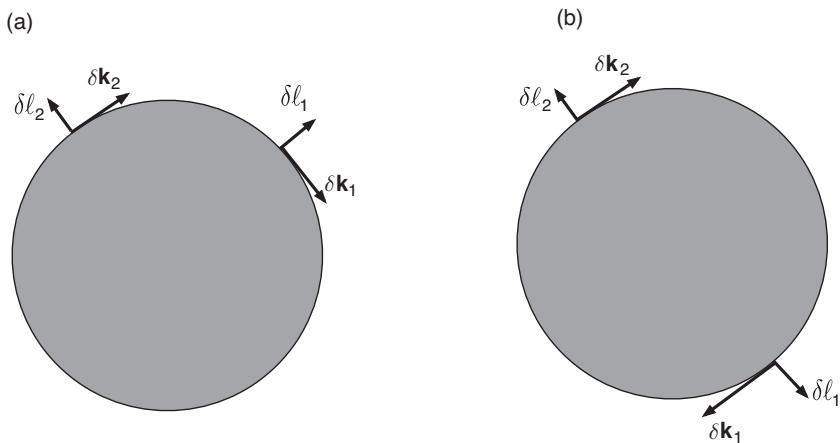
\includegraphics[width=0.62\textwidth]{figs/ch12/fig_12.13.jpg}
\caption*{图 12.13\quad（a）两个电子一般地位于费米面上的动量。（b）此处两动量相反，即 $\mathbf p_1=-\mathbf p_2$。这时 $\delta\mathbf k_1$ 与 $\delta\mathbf k_2$ 平行，且 $\delta\boldsymbol\ell_1$ 与 $\delta\boldsymbol\ell_2$ 指向恰好相反的方向。}\label{fig:auto:12.13}
\end{figure}

当诸 $\delta\mathbf k_i$ 线性无关时，$\delta$ 函数可以像之前那样处理。具体地说，它不参与标度，我们之前的结论——四费米子相互作用是无关的——依然成立。考虑图 12.13b 所示的情形，其中 $\mathbf p_1=-\mathbf p_2$，因而 $\delta\mathbf k_3$ 与 $\delta\mathbf k_4$ 彼此平行。此时，维持动量守恒的 $\delta$ 函数
\begin{equation*}
\delta^d\left(\delta\mathbf k_3+\delta\mathbf k_4\right)\delta^d\left(\delta\boldsymbol\ell_3+\delta\boldsymbol\ell_4\right), \tag{12.106}
\end{equation*}
发生因子化，因为 $\delta\boldsymbol\ell_3$ 与 $\delta\boldsymbol\ell_4$ 都垂直于 $\delta\mathbf k_3$ 与 $\delta\mathbf k_4$。在标度 $\ell\to s\ell$ 下，两个 $\delta$ 函数中的第二个按 $s^{-1}$ 标度。该因子抵消了先前导出的线性 $s$ 因子。因此我们相当普遍地发现：当这对电子的净动量为零时，四费米子相互作用既不相关也非无关，而是按 $s^0$ 标度，因而是边际的。

那么这把我们置于何地？当电子散射到宇称对称的动量态时，我们需要更加努力地弄清费米面的命运。为此，我们计算一阶修正，希望构造一个类似于近藤问题中交换耦合的递推关系。到 $V^2$ 阶，相关的图示于图 12.14。第一张图就是裸电子–电子相互作用顶点。第二张图是精确到相互作用二阶的顶点。我们赋予气泡（即图中的诸线）的每条内部费米子线一个形式为 $1/(E-v_{\mathrm F}\ell)$ 的传播子，其中 $E$ 是内部费米子线的能量。二阶顶点取如下形式
\begin{equation*}
V^2\int\frac{\mathrm d E'\,\mathrm d^2\mathbf k\,\mathrm d\ell'}{2\pi^4}\frac{1}{\left[(1+\mathrm i\epsilon)(E+E')-v_{\mathrm F}(\mathbf k')\ell'\right]\left[(1+\mathrm i\epsilon)(E-E')-v_{\mathrm F}(\mathbf k')\ell'\right]}. \tag{12.107}
\end{equation*}

\begin{figure}[H]\centering
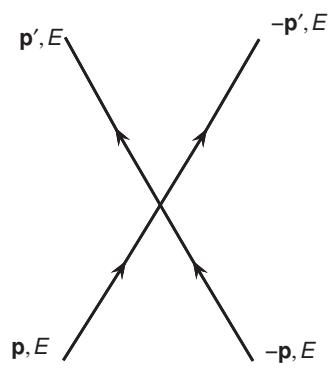
\includegraphics[width=0.40\textwidth]{figs/ch12/fig_12.14_a.jpg}\hfill
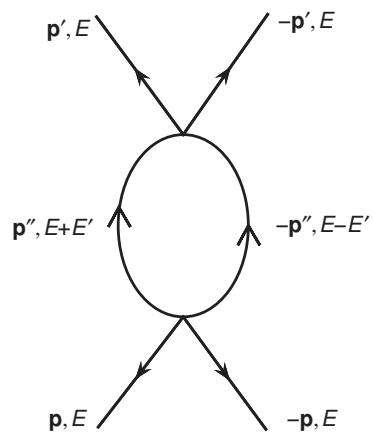
\includegraphics[width=0.40\textwidth]{figs/ch12/fig_12.14_b.jpg}
\caption*{图 12.14\quad（a）处于态 $(\mathbf p,E)$ 与 $(-\mathbf p,E)$ 的电子散射到 $(-\mathbf p',E)$ 与 $(-\mathbf p',E)$ 的裸相互作用顶点；（b）$O(V^2)$ 顶点。与该顶点对应的积分在式 (12.107) 中计算。}\label{fig:auto:12.14}
\end{figure}

$(1+\mathrm i\epsilon)$ 因子的作用是正规化积分。最后我们将取 $\epsilon\to 0$ 极限。在计算气泡顶点中的积分时，把分母改写为
\begin{equation*}
\frac{-1}{(1+2\mathrm i\epsilon)\left[E'+E-(1-\mathrm i\epsilon)v_{\mathrm F}(\mathbf k')\ell'\right]\left[E'-E+(1-\mathrm i\epsilon)v_{\mathrm F}(\mathbf k')\ell'\right]}, \tag{12.108}
\end{equation*}
会有所帮助，其中我们明确地做了近似 $(1+\mathrm i\epsilon)^2\approx(1+2\mathrm i\epsilon)$，因为 $\epsilon$ 严格属于 $O(0)$ 阶。为计算该积分，我们在上半平面闭合围道。有两个我们感兴趣的极点，位于
\begin{equation*}
E'=\pm E\mp v_{\mathrm F}(\mathbf k')\ell'\pm\mathrm i\epsilon v_{\mathrm F}(\mathbf k')\ell', \tag{12.109}
\end{equation*}
其中上号对应 $\ell'>0$，下号对应 $\ell'<0$，这样两个极点都位于上半平面。利用每个极点处的留数为
\begin{equation*}
\frac{2\pi\mathrm i}{\pm 2E\mp 2v_{\mathrm F}(\mathbf k')\ell'\pm 2\mathrm i\epsilon v_{\mathrm F}(\mathbf k')\ell'}, \tag{12.110}
\end{equation*}
这一事实，我们把二阶顶点化为
\begin{equation*}
\frac{-\mathrm i V^2}{2}N\left[\int_0^{E_0}\frac{\mathrm d b}{E-b+\mathrm i\epsilon}+\int_{-E_0}^{0}\frac{\mathrm d b}{b-E-\mathrm i\epsilon}\right], \tag{12.111}
\end{equation*}
其中已换元 $b=v_{\mathrm F}(\mathbf k')\ell'$，并定义了
\begin{equation*}
N=\int\frac{\mathrm d^2\mathbf k'}{(2\pi)^3}\frac{1}{v_{\mathrm F}(\mathbf k')}, \tag{12.112}
\end{equation*}
同时忽略了正比于无穷小量 $\epsilon$ 的各项之前的任何前置因子。每个积分都给出一个对数：
\begin{equation*}
\mathrm i V^2N\ln\left(\frac{E_0}{|E|}\right). \tag{12.113}
\end{equation*}
注意到裸四费米子顶点正比于 $-\mathrm i V$，精确到二阶的有效相互作用变为
\begin{equation*}
V(E)=V-V^2N\left(\ln\left(\frac{E_0}{|E|}\right)+O(1)\right)+O(V^3). \tag{12.114}
\end{equation*}
我们对这个等式的两边求导，
\begin{equation*}
\frac{\mathrm d V(E)}{\mathrm d E}=NV(E)^2/E, \tag{12.115}
\end{equation*}
得到相互作用顶点的标度方程。这个方程与第 8 章近藤问题中导出的交换相互作用增长的标度方程完全相同。该方程的解就是
\begin{equation*}
V(E)=\frac{V}{1+NV\ln(E_0/E)}. \tag{12.116}
\end{equation*}
我们清楚地看到：对于正的裸相互作用 $V>0$，有效相互作用在低能（即 $E<E_0$）处减小。然而，对 $V<0$，相互作用增大。这就是 BCS 失稳，也是如下的基本论断：除短程吸引外，所有重正化都朝向费米面。注意，裸相互作用 $V$ 是真正的边际量。因此，BCS 理论中的超导电性是边际耦合变大并在强耦合处产生新自由度（即电子对凝聚）的一个例子。

BCS 超导配对理论的一个关键假设是：正常态的性质由具有无穷寿命 [L1964; L1965] 的无相互作用准粒子描述，且这些准粒子与裸电子一一对应。这一假设得到刚才给出的标度分析的支持，也在从 I 类到 II 类的众多材料的正常态中得到实验支持。由于正常态本质上无相互作用，某个准粒子的能量就是把该粒子加入或移出系统某个态所需的能量。为说明这一概念，考虑一个由某分布函数 $n^0_{\mathbf p\sigma}$（一般取为费米–狄拉克分布）描述的相互作用系统。设想以极其缓慢的方式向系统加入或移出一个粒子，使系统始终处于基态。这一过程代表粒子数的绝热改变。尽管如此，这一过程会把粒子分布改变为某个新量 $n_{\mathbf p\sigma}$，从而基态能量也随之改变。设 $\delta n_{\mathbf p\sigma}$ 表示粒子分布函数的相应改变。我们可以把基态能量的变化
\begin{equation*}
\delta E=\frac{1}{V}\sum_{\mathbf p\sigma}\epsilon_{\mathbf p\sigma}\delta n_{\mathbf p\sigma}+\frac{1}{2V^2}\sum_{\mathbf p\sigma,\mathbf p'\sigma'}f_{\mathbf p\sigma,\mathbf p'\sigma'}\delta n_{\mathbf p\sigma}\delta n_{\mathbf p'\sigma'}+\cdots, \tag{12.117}
\end{equation*}
按涨落 $\delta n_{\mathbf p\sigma}$ 的幂次展开而计算出来。朗道 [L1956] 参量 $f_{\mathbf p\sigma,\mathbf p'\sigma'}$ 描述准粒子之间如何相互作用。该量在 $\mathbf p$ 与 $\mathbf p'$ 互换下不变。我们把准粒子的能量
\begin{equation*}
\tilde\epsilon_{\mathbf p\sigma}=\epsilon_{\mathbf p\sigma}+\frac{1}{V}\sum_{\mathbf p'\sigma'}f_{\mathbf p\sigma,\mathbf p'\sigma'}\delta n_{\mathbf p'\sigma'}+\cdots, \tag{12.118}
\end{equation*}
通过对新基态能量关于 $\delta n_{\mathbf p\sigma}$ 求变分而识别出来。于是我们清楚地看到，准粒子能量本身是分布函数的函数。更明确地说，准粒子服从费米–狄拉克分布函数，只是把 $\epsilon_{\mathbf p}-\mu$ 换成了 $\tilde\epsilon_{\mathbf p_\sigma}-\mu$。在费米面上，准粒子以下列速度运动：
\begin{equation*}
v_{\mathrm F}=\left(\frac{\partial\epsilon_{\mathbf p\sigma}}{\partial\mathbf p}\right)_{p=p_{\mathrm F}} \tag{12.119}
\end{equation*}
它等于费米速度。因为 $v_{\mathrm F}=p_{\mathrm F}/m^*$，准粒子有效质量的形式定义为
\begin{equation*}
\frac{1}{m^*}=\frac{1}{p_{\mathrm F}}\left(\frac{\partial\epsilon_{\mathbf p\sigma}}{\partial\mathbf p}\right)_{p=p_{\mathrm F}}. \tag{12.120}
\end{equation*}
因此在费米面附近，准粒子能量
\begin{equation*}
\epsilon_{\mathbf p\sigma}=\epsilon_{\mathrm F}+v_{\mathrm F}(p-p_{\mathrm F}) \tag{12.121}
\end{equation*}
对位移动量 $p-p_{\mathrm F}$ 是线性的。由于我们的大部分关注点都在费米面附近的过程，这个表达式应当足以描述准粒子的能量。

\section{配对振幅}

此时按惯例应当写下 BCS 波函数，然后一路高歌猛进地去阐明超导转变。然而，我们想退后一步，考察库珀对的配对振幅（pair amplitude）的期望值。这样做了之后，我们将能够“骗过”（swindle）BCS 理论。迄今我们已经确立：若温度足够低，费米面上方的两个电子可以通过形成恰在 $\epsilon_{\mathrm F}$ 下方的束缚单态库珀原来降低能量。这告诉我们，应当能够定义一个序参量，其期望值能够判别库珀失稳是否已经发生。对 $(\mathbf p\uparrow,-\mathbf p\downarrow)$ 对，适当的配对算符是
\begin{equation*}
b^\dagger_{\mathbf p}=a^\dagger_{\mathbf p\uparrow}a^\dagger_{-\mathbf p\downarrow}, \tag{12.122}
\end{equation*}
而
\begin{equation*}
b_{\mathbf p}=a_{-\mathbf p\downarrow}a_{\mathbf p\uparrow} \tag{12.123}
\end{equation*}
是相应的对湮灭算符。设 $|N\rangle$ 表示 $N$ 粒子系统的基态。库珀失稳暗示在超导态 $\langle N-2|b_{\mathbf p}|N\rangle\neq 0$。让我们定义
\begin{equation*}
\alpha_{\mathbf p}=\langle N-2|b_{\mathbf p}|N\rangle, \tag{12.124}
\end{equation*}
它一般被称为配对振幅。我们将证明：在某个特定温度以下，$\alpha_{\mathbf p}$ 指数式增长。在正常态，$\alpha_{\mathbf p}$ 等于 1 或 0。在 BCS 理论中，$\alpha_{\mathbf p}$ 与序参量密切相关。

我们首先证明 $\alpha_{\mathbf p}$ 是对态的一般展开系数。为此，我们把一般单态对态写为
\begin{equation*}
|\psi\rangle=\sum_{\mathbf p>\mathbf p_{\mathrm F}}\eta_{\mathbf p}b^\dagger_{\mathbf p}|0\rangle=\sum_{\mathbf p>\mathbf p_{\mathrm F}}\eta_{\mathbf p}|\mathbf p\uparrow-\mathbf p\downarrow\rangle, \tag{12.125}
\end{equation*}
其中 $\eta_{\mathbf p}$ 是展开系数。为确定 $\eta_{\mathbf p}$，注意
\begin{align*}
\langle 0|b_{\mathbf p}|\psi\rangle&=\sum_{\mathbf p'}\eta_{\mathbf p'}\langle 0|b_{\mathbf p}b^\dagger_{\mathbf p'}|0\rangle\\
&=\sum_{\mathbf p'}\eta_{\mathbf p'}\delta_{\mathbf p\mathbf p'}=\eta_{\mathbf p}. \tag{12.126}
\end{align*}
因为 $|\psi\rangle$ 与 $|0\rangle$ 只相差两个粒子，故 $\eta_{\mathbf p}=\alpha_{\mathbf p}$。

配对振幅是一般配对态的展开系数。让我们计算 $\alpha_{\mathbf p}$ 的时间演化。为此，我们把 BCS 哈密顿量写作
\begin{equation*}
H=H_0+H_{\mathrm{int}}, \tag{12.127}
\end{equation*}
其中
\begin{align*}
H_0&=\sum_{\mathbf p,\sigma}\epsilon_{\mathbf p}a^\dagger_{\mathbf p\sigma}a_{\mathbf p\sigma}\\
H_{\mathrm{int}}&=\sum_{\mathbf p\mathbf p'}V_{\mathbf p\mathbf p'}b^\dagger_{\mathbf p}b_{\mathbf p'}. \tag{12.128}
\end{align*}
在薛定谔绘景中，$\alpha_{\mathbf p}$ 的时间依赖由波函数承载。于是
\begin{align*}
\mathrm i\hbar\frac{\partial}{\partial t}\alpha_{\mathbf p}(t)&=\mathrm i\hbar\frac{\partial}{\partial t}\big\langle 0(t)\left|b_{\mathbf p}\right|\psi(t)\big\rangle\\
&=\big\langle 0(t)\left|\left[b_{\mathbf p},H\right]\right|\psi(t)\big\rangle. \tag{12.129}
\end{align*}
为计算 $[b_{\mathbf p},H]$，下列对易子将是有用的：
\begin{align*}
&\left[b_{\mathbf p},n_{\mathbf p'\sigma}\right]=b_{\mathbf p}\left(\delta_{\mathbf p\mathbf p'}\delta_{\sigma\uparrow}+\delta_{\mathbf p,-\mathbf p'}\delta_{\sigma\downarrow}\right),\\
&\Big[b_{\mathbf p},b^\dagger_{\mathbf p'}\Big]=\delta_{\mathbf p\mathbf p'}\left(1-n_{\mathbf p\uparrow}-n_{-\mathbf p\downarrow}\right). \tag{12.130}
\end{align*}
我们清楚地看到，占据因子 $n_{\mathbf p\uparrow}+n_{-\mathbf p\downarrow}$ 使诸对产生算符互不对易。这些项维护了组成对的电子之间的泡利原理。现在我们可以计算 $[b_{\mathbf p},H]$：
\begin{align*}
[b_{\mathbf p},H]&=\sum_{\mathbf p'\sigma}\left[b_{\mathbf p},\epsilon_{\mathbf p'}n_{\mathbf p'\sigma}\right]+\sum_{\mathbf p\mathbf p'}V_{\mathbf p\mathbf p'}\left[b_{\mathbf p},b^\dagger_{\mathbf p'}b_{\mathbf p'}\right]\\
&=2\epsilon_{\mathbf p}b_{\mathbf p}+{\sum_{\mathbf p}}'V_{\mathbf p\mathbf p'}\left(1-n_{-\mathbf p\downarrow}-n_{\mathbf p\uparrow}\right)b_{\mathbf p'}. \tag{12.131}
\end{align*}
求和上的撇号表示限制在 $\epsilon_{\mathrm F}$ 附近宽度为 $2\hbar\omega_{\mathrm D}$ 的薄动量壳层内求和。通过注意 $\left(1-n_{-\mathbf p\downarrow}-n_{\mathbf p\uparrow}\right)=\left(1-n_{\mathbf p\uparrow}\right)\left(1-n_{-\mathbf p\downarrow}\right)-n_{\mathbf p\uparrow}n_{-\mathbf p\downarrow}$，我们可以对这个结果获得物理洞察。把此结果用于式 (12.131)，我们得到
\begin{equation*}
\left(\mathrm i\hbar\frac{\partial}{\partial t}-2\epsilon_{\mathbf p}\right)\alpha_{\mathbf p}(t)=\left[\left(1-n_{\mathbf p\uparrow}\right)\left(1-n_{-\mathbf p\downarrow}\right)-n_{\mathbf p\uparrow}n_{-\mathbf p\downarrow}\right]{\sum_{\mathbf p'}}'V_{\mathbf p\mathbf p'}\alpha_{\mathbf p'}(t) \tag{12.132}
\end{equation*}
作为配对振幅的时间演化。组成对的粒子处于费米面之外的概率由乘积 $\left(1-n_{\mathbf p\uparrow}\right)\left(1-n_{-\mathbf p\downarrow}\right)$ 决定，而 $n_{\mathbf p\uparrow}n_{-\mathbf p\downarrow}$ 是它们位于面内的概率。如果我们严格只关心像库珀问题中那样恰在费米面之外的两个动量态之间的配对，这一项可以忽略。在此极限下，我们的有效运动方程为
\begin{equation*}
\left(\mathrm i\hbar\frac{\partial}{\partial t}-2\epsilon_{\mathbf p}\right)\alpha_{\mathbf p}(t)=\left(1-n_{\mathbf p\uparrow}\right)\left(1-n_{-\mathbf p\downarrow}\right){\sum_{\mathbf p'}}'V_{\mathbf p\mathbf p'}\alpha_{\mathbf p'}(t) \tag{12.133}
\end{equation*}
因为 $\mathrm i\hbar\partial/\partial t\to E$，上式正是我们先前为确定库珀束缚态能量所解的薛定谔方程。然而，一般的配对振幅方程，即式 (12.132)，要求所有粒子都参与配对过程，无论它们位于费米面之内还是之外。这就是 BCS 理论的精髓。库珀只包含了 $\epsilon_{\mathrm F}$ 之外的粒子，而 BCS 只是额外纳入了 $n_{\mathbf p\uparrow}n_{-\mathbf p\downarrow}$ 项。这一简单的改动带来了天壤之别。

\subsection{失稳：超导态}

我们转向配对振幅的计算。我们想证明：在某个特征温度 $T_{\mathrm c}$ 以下，配对振幅指数式增长。我们寻求如下形式的解
\begin{equation*}
\alpha_{\mathbf p}(t)=\mathrm e^{-\mathrm i\frac{zt}{\hbar}}\alpha_{\mathbf p}(t=0). \tag{12.134}
\end{equation*}
把它代入配对方程，我们得到
\begin{equation*}
\left(z-2\epsilon_{\mathbf p}\right)\alpha_{\mathbf p}(0)=\left(1-n_{\mathbf p\uparrow}-n_{-\mathbf p\downarrow}\right){\sum_{\mathbf p'}}'V_{\mathbf p\mathbf p'}\alpha_{\mathbf p'}(0) \tag{12.135}
\end{equation*}
作为配对振幅方程的傅里叶变换。

对于式 (12.51) 的模型吸引势，配对振幅演化方程变为
\begin{equation*}
\left(z-2\epsilon_{\mathbf p}\right)\alpha_{\mathbf p}(0)=-V_0\left(1-n_{\mathbf p\uparrow}-n_{-\mathbf p\downarrow}\right){\sum_{\mathbf p'}}'\alpha_{\mathbf p'}(0). \tag{12.136}
\end{equation*}
和之前一样，我们对这个表达式两边求和，得到
\begin{equation*}
{\sum_{\mathbf p}}'\alpha_{\mathbf p}(0)=-V_0{\sum_{\mathbf p}}'\frac{\left(1-n_{\mathbf p\uparrow}-n_{-\mathbf p\downarrow}\right)}{z-2\epsilon_{\mathbf p}}{\sum_{\mathbf p'}}\alpha_{\mathbf p'}(0), \tag{12.137}
\end{equation*}
这意味着
\begin{equation*}
1=-V_0{\sum_{\mathbf p}}'\frac{\left(1-n_{\mathbf p\uparrow}-n_{-\mathbf p\downarrow}\right)}{z-2\epsilon_{\mathbf p}}. \tag{12.138}
\end{equation*}
这与我们之前的表达式几乎相同，只是现在把所有粒子之间的配对都包括了进来。为得到解，我们画出上述方程左、右两边的交点。和之前一样，我们在离散能量 $\epsilon_{\mathbf p}$ 附近画出右端。

显而易见，只有当 $2\epsilon_{\mathrm F}-2\hbar\omega_{\mathrm D}\leq\mathrm{Re}\,z\leq 2\epsilon_{\mathrm F}+2\hbar\omega_{\mathrm D}$ 时解才存在。为求解配对条件，我们把求和化为积分，并注意对自由粒子有 $n_{\mathbf p}=n_{-\mathbf p}$。另外，由于 $\epsilon_{\mathbf p\uparrow}=\epsilon_{\mathbf p\downarrow}$，立即得到
\begin{equation*}
n_{\mathbf p\uparrow}=n_{-\mathbf p\downarrow}=\left(\mathrm e^{\beta(\epsilon_{\mathbf p}-\mu)}+1\right)^{-1} \tag{12.139}
\end{equation*}
以及
\begin{equation*}
1=-V_0N\left(\epsilon_{\mathrm F}\right)\int_{-\hbar\omega_{\mathrm D}}^{\hbar\omega_{\mathrm D}}\mathrm d\epsilon\,\frac{\tanh\beta\epsilon/2}{z-2\mu-2\epsilon}, \tag{12.140}
\end{equation*}
其中 $N(\epsilon_{\mathrm F})$ 是费米能级处的态密度。若 $z$ 具有正的虚部，配对振幅将指数增长。令 $z=2\mu+x+\mathrm i y$，$x$ 与 $y$ 为实数。首先考虑 $y=0$ 的情形。在此极限下我们得到
\begin{equation*}
1=-V_0N\left(\epsilon_{\mathrm F}\right)\int_{-\hbar\omega_{\mathrm D}}^{\hbar\omega_{\mathrm D}}\mathrm d\epsilon\,\tanh\frac{\beta\epsilon}{2}\left[P\left(\frac{1}{x-2\epsilon}\right)-\mathrm i\pi\delta\left(x-2\epsilon\right)\right]. \tag{12.141}
\end{equation*}
为满足这个方程，虚部必须为零。这只有在 $|x|/2>\hbar\omega_{\mathrm D}$ 时才成立，等价地 $\mathrm{Re}\,z>2\epsilon_{\mathrm F}+2\hbar\omega_{\mathrm D}$。如图 12.15 所示，在这个能量范围内被积函数的实部为正。因此，$y=0$ 不被允许。

要使解存在于能量壳层上，必须 $y\neq 0$。我们把配对约束写成
\begin{equation*}
1=-V_0N\left(\epsilon_{\mathrm F}\right)\int_{-\hbar\omega_{\mathrm D}}^{\hbar\omega_{\mathrm D}}\frac{\left(x-2\epsilon-\mathrm i y\right)}{\left(x-2\epsilon\right)^2+y^2}\tanh\frac{\beta\epsilon}{2}\,\mathrm d\epsilon, \tag{12.142}
\end{equation*}

\begin{figure}[H]\centering
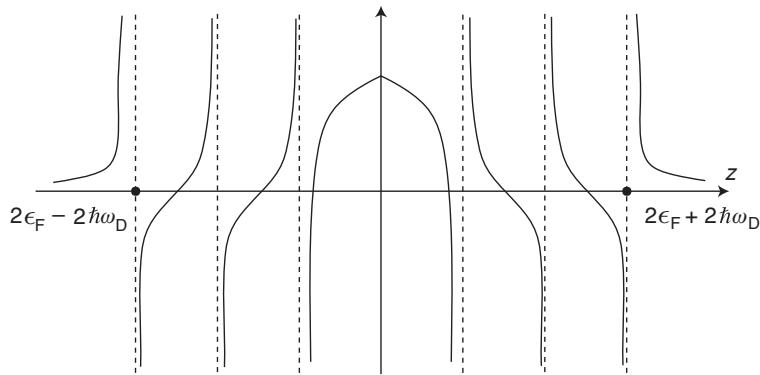
\includegraphics[width=0.62\textwidth]{figs/ch12/fig_12.15.jpg}
\caption*{图 12.15\quad 配对振幅方程的右端作为复能量 $z$ 的函数。}\label{fig:auto:12.15}
\end{figure}

这只有在虚部
\begin{equation*}
\int_{-\hbar\omega_{\mathrm D}}^{\hbar\omega_{\mathrm D}}\frac{\tanh\beta\epsilon/2\,\mathrm d\epsilon}{\left(x-2\epsilon\right)^2+y^2}, \tag{12.143}
\end{equation*}
为零时才成立。因为 $\tanh(x)=-\tanh(-x)$，我们把被积函数改写为
\begin{align*}
0&=\frac{1}{2}\int_{-\hbar\omega_{\mathrm D}}^{\hbar\omega_{\mathrm D}}\mathrm d\epsilon\,\tanh\frac{\beta\epsilon}{2}\left[\frac{1}{\left(x-2\epsilon\right)^2+y^2}-\frac{1}{\left(x+2\epsilon\right)^2+y^2}\right]\\
&=\frac{1}{2}\int_{-\hbar\omega_{\mathrm D}}^{\hbar\omega_{\mathrm D}}\mathrm d\epsilon\,\tanh\frac{\beta\epsilon}{2}\left[\frac{8\epsilon x}{\left(\left(x-2\epsilon\right)^2+y^2\right)\left(\left(x+2\epsilon\right)^2+y^2\right)}\right]. \tag{12.144}
\end{align*}
现在清楚 $x=0$，因为 $\epsilon\tanh\beta\epsilon/2$ 处处为正。因此，我们的解必须形如 $z=2\mu+\mathrm i y$。于是我们必须求解
\begin{equation*}
1=-N\left(\epsilon_{\mathrm F}\right)V_0\int_{-\hbar\omega_{\mathrm D}}^{\hbar\omega_{\mathrm D}}\mathrm d\epsilon\,\frac{\left(-\mathrm i y-2\epsilon\right)\tanh\beta\epsilon/2}{4\epsilon^2+y^2}. \tag{12.145}
\end{equation*}
该积分的虚部关于 $\epsilon$ 为奇，从而严格为零。我们剩下单独一个方程
\begin{equation*}
1=4N\left(\epsilon_{\mathrm F}\right)V_0\int_0^{\hbar\omega_{\mathrm D}}\mathrm d\epsilon\,\frac{\epsilon\tanh\beta\epsilon/2}{4\epsilon^2+y^2}. \tag{12.146}
\end{equation*}
这里被积函数同样是正的。随着 $y$ 增大，被积函数减小。$T$ 增大时也是如此。因此，当 $T$ 大于某个温度时不存在解。这就定义了临界温度 $T_{\mathrm c}$。当 $T\to 0$，我们发现
\begin{align*}
1&=\frac{N\left(\epsilon_{\mathrm F}\right)V_0}{2}\int_0^{(2\hbar\omega_{\mathrm D})^2}\frac{\mathrm d a}{a+y^2}\\
&=\frac{N\left(\epsilon_{\mathrm F}\right)V_0}{2}\ln\left(\frac{(2\hbar\omega_{\mathrm D})^2+y^2}{y^2}\right). \tag{12.147}
\end{align*}
对该方程的两边取指数，
\begin{align*}
y^2&=\left(2\hbar\omega_{\mathrm D}\right)^2\left(\exp\left(\frac{2}{N\left(\epsilon_{\mathrm F}\right)V_0}\right)-1\right)^{-1}\\
&\approx\left(2\hbar\omega_{\mathrm D}\right)^2\exp\left(-\frac{2}{N\left(\epsilon_{\mathrm F}\right)V_0}\right), \tag{12.148}
\end{align*}
得到 $y$ 的熟悉方程，即
\begin{equation*}
y=\pm 2\hbar\omega_{\mathrm D}\exp\left(-\frac{1}{N\left(\epsilon_{\mathrm F}\right)V_0}\right). \tag{12.149}
\end{equation*}
选取正解，我们得出结论：当 $T\to 0$ 时，配对振幅按下式增长：
\begin{align*}
\alpha_{\mathbf p}(t)&\simeq\mathrm e^{-\mathrm i zt}\\
&=\mathrm e^{-2\mathrm i\mu t}\,\mathrm e^{2\hbar\omega_{\mathrm D}t\exp(-1/N(\epsilon_{\mathrm F})V_0)}. \tag{12.150}
\end{align*}
配对振幅指数增长的存在是 $N$ 粒子基态失稳的标志。我们仅仅聚焦于配对振幅 $\alpha_{\mathbf p}$ 就基本上导出了 BCS 理论。为得到 $T_{\mathrm c}$ 的精确表达式，我们在 $y=0$ 的极限下考虑配对结合方程。在此极限下，满足式 (12.146) 的温度最大。因此，$y=0$ 的解可以用来估计 $T_{\mathrm c}$。让我们定义 $\beta_{\mathrm c}=1/k_{\mathrm B}T_{\mathrm c}$。我们发现
\begin{equation*}
1=N\left(\epsilon_{\mathrm F}\right)V_0\int_0^{\hbar\omega_{\mathrm D}\beta_{\mathrm c}/2}\frac{\tanh x}{x}\,\mathrm d x. \tag{12.151}
\end{equation*}
这个积分必须数值完成。与式 (12.151) 一致的转变温度为
\begin{equation*}
k_{\mathrm B}T_{\mathrm c}=1.14\,\hbar\omega_{\mathrm D}\exp\left(-\frac{1}{N\left(\epsilon_{\mathrm F}\right)V_0}\right). \tag{12.152}
\end{equation*}
我们将证明，参数 $y$ 在 BCS 理论中扮演能隙的角色。

\section{BCS 基态}

迄今我们已经展示了配对假设如何在 $T<T_{\mathrm c}$ 时导致基态失稳。现在的焦点是描述这个态的多粒子波函数。我们分析的出发点是 $N$ 个无相互作用电子的多体态：
\begin{equation*}
|\Psi^0(N)\rangle=\prod_{\mathbf p<\mathbf p_{\mathrm F}}b^\dagger_{\mathbf p}|0\rangle. \tag{12.153}
\end{equation*}
由于每个动量态都被双重占据，我们可以用配对算符 $b^\dagger_{\mathbf p}$ 逐次作用于真空来构造这个态。放开 $\mathbf p<\mathbf p_{\mathrm F}$ 的限制，我们把 $|\Psi^0(N)\rangle$ 改写为
\begin{equation*}
\left|\Psi^0\left(N\right)\right.\rangle=\prod_{\mathbf p}\left(u^0_{\mathbf p}+v^0_{\mathbf p}b^\dagger_{\mathbf p}\right)\left|0\right.\rangle, \tag{12.154}
\end{equation*}
其中
\begin{equation*}
u^0_{\mathbf p}=\begin{cases}0, & \mathbf p<\mathbf p_{\mathrm F},\\ 1, & \mathbf p>\mathbf p_{\mathrm F},\end{cases} \tag{12.155}
\end{equation*}
\begin{equation*}
v^0_{\mathbf p}=\begin{cases}1, & \mathbf p<\mathbf p_{\mathrm F},\\ 0, & \mathbf p>\mathbf p_{\mathrm F}.\end{cases} \tag{12.156}
\end{equation*}
$|\Psi^0\rangle$ 的这个表示与式 (12.153) 相同。还要注意，由于诸 $a^\dagger_{\mathbf p}$ 彼此反对易，$|\Psi^0(N)\rangle$ 是恰当反对称化的。

BCS 假定一般的电子超导基态可以写成
\begin{equation*}
|\Psi_{\mathrm{BCS}}\rangle=\prod_{\mathbf p}\left(u_{\mathbf p}+v_{\mathbf p}b^\dagger_{\mathbf p}\right)|0\rangle, \tag{12.157}
\end{equation*}
其中系数 $u_{\mathbf p}$ 与 $v_{\mathbf p}$ 待变分确定，被称为相干因子（coherence factors）。归一化条件 $\langle\Psi_{\mathrm{BCS}}|\Psi_{\mathrm{BCS}}\rangle=1$ 施加约束
\begin{equation*}
1=\langle 0|\prod_{\mathbf p,\mathbf p'}\left(u^*_{\mathbf p}+v^*_{\mathbf p}b_{\mathbf p}\right)\left(u_{\mathbf p'}+v_{\mathbf p'}b^\dagger_{\mathbf p'}\right)|0\rangle. \tag{12.158}
\end{equation*}
式 (12.158) 中出现的这类乘积可以利用式 (12.130) 的对易关系并注意 $b_{\mathbf p}b^\dagger_{\mathbf p}|0\rangle=1$ 来简化。我们发现只有对角 $\left(p=p'\right)$ 项存活：
\begin{equation*}
\langle\Psi_{\mathrm{BCS}}|\Psi_{\mathrm{BCS}}\rangle=\prod_{\mathbf p}\left(\left|u_{\mathbf p}\right|^2+\left|v_{\mathbf p}\right|^2\right), \tag{12.159}
\end{equation*}
这意味着
\begin{equation*}
\left|u_{\mathbf p}\right|^2+\left|v_{\mathbf p}\right|^2=1. \tag{12.160}
\end{equation*}
如果把 BCS 基态中的乘积展开，显然 $|\Psi_{\mathrm{BCS}}\rangle$ 是所有 $2m$ 粒子态的和
\begin{equation*}
|\Psi_{\mathrm{BCS}}\rangle=\sum_m A_{2m}|\Psi_{2m}\rangle, \tag{12.161}
\end{equation*}
其中 $m$ 为整数，$A_{2m}$ 是展开系数，$|\Psi_{2m}\rangle$ 是 $2m$ 个粒子的基态。我们可以通过把展开系数 [S1964] 写成 $A_{2m}=|A_{2m}|\mathrm e^{2\mathrm i m\phi}$ 来建立 $|\Psi_{2m}\rangle$ 与 $|\Psi_{\mathrm{BCS}}\rangle$ 的联系，于是
\begin{equation*}
\left|\Psi^{\phi}_{\mathrm{BCS}}\right.\rangle=\sum_m\mathrm e^{2\mathrm i m\phi}|A_{2m}||\Psi_{2m}\rangle. \tag{12.162}
\end{equation*}
也就是说，我们赋予每个 $2m$ 粒子态一个整体相位 $2m\phi$。为此，通过给每个对产生算符乘上 $\exp(2\mathrm i\phi)$，我们把 BCS 基态改写为
\begin{equation*}
\left|\Psi^{\phi}_{\mathrm{BCS}}\right.\rangle=\prod_{\mathbf p}\left(u_{\mathbf p}+\mathrm e^{2\mathrm i\phi}v_{\mathbf p}b^\dagger_{\mathbf p}\right)\left|0\right.\rangle \tag{12.163}
\end{equation*}
把式 (12.162) 乘以 $\exp(-\mathrm i 2m\phi)$ 并对 $\phi$ 积分，我们得到每个 $2m$ 粒子态与 BCS 基态之间的简洁关系
\begin{equation*}
\left|\Psi_{2m}\right.\rangle=\frac{1}{2\pi\left|A_{2m}\right|}\int_0^{2\pi}\mathrm d\phi\,\mathrm e^{-\mathrm i 2m\phi}\prod_{\mathbf p}\left(u_{\mathbf p}+\mathrm e^{2\mathrm i\phi}v_{\mathbf p}b^\dagger_{\mathbf p}\right)\left|0\right.\rangle \tag{12.164}
\end{equation*}
在式 (12.164) 的右端只有 $2m$ 粒子的态存活，这源于如下事实：
\begin{equation*}
\frac{1}{2\pi}\int_0^{2\pi}\mathrm e^{\mathrm i\phi(N-N')}\mathrm d\phi=\delta_{NN'}. \tag{12.165}
\end{equation*}
由于诸 $2m$ 粒子态相互正交，当我们用 $\langle\Psi_{2m}|$ 乘式 (12.164) 时，左边变为 1，从而可以识别出展开系数的平方为
\begin{align*}
|A_{2m}|^2&=\int_0^{2\pi}\int_0^{2\pi}\frac{\mathrm d\phi}{2\pi}\frac{\mathrm d\phi'}{2\pi}\,\mathrm e^{-\mathrm i 2m(\phi-\phi')}\langle 0|\prod_{\mathbf p,\mathbf p'}\left(u^*_{\mathbf p}+\mathrm e^{-2\mathrm i\phi'}v^*_{\mathbf p}b_{\mathbf p}\right)\left(u_{\mathbf p'}+\mathrm e^{2\mathrm i\phi}v_{\mathbf p'}b^\dagger_{\mathbf p'}\right)|0\rangle\\
&=\frac{1}{2\pi}\int_0^{2\pi}\mathrm d\phi\,\mathrm e^{-2\mathrm i m\phi}\prod_{\mathbf p}\left(\left|u_{\mathbf p}\right|^2+\mathrm e^{2\mathrm i\phi}\left|v_{\mathbf p}\right|^2\right). \tag{12.166}
\end{align*}
式 (12.166) 应被理解为 BCS 态中 $2m$ 个粒子的概率分布。这个量在 BCS 态的平均粒子数处强烈峰化，其宽度正比于系统中平均粒子数的平方根（见习题 12.8）。

我们把 BCS 态改写为所有可能的 $2m$ 粒子态（都具有同一相位 $\phi$）的线性叠加，这暗示在超导态中相位与粒子数之间存在共轭关系。确实存在这样的关系。然而，若其中一个变量有下界，这样的关系便不可能存在。不失一般性，我们可以把粒子数当作 $-\infty<N<\infty$ 的连续变量来处理。我们可以直截了当地建立这一共轭关系：对式 (12.164) 中的 $\left|\psi^{\phi}_{\mathrm{BCS}}\right.\rangle$ 作用 $-\mathrm i\partial/\partial\phi$，然后分部积分。结果
\begin{equation*}
\frac{1}{2\pi|A_{2m}|}\int_0^{2\pi}\mathrm d\phi\,\mathrm e^{-\mathrm i 2m\phi}\frac{-\mathrm i\partial}{\partial\phi}\prod_{\mathbf p}\left(u_{\mathbf p}+\mathrm e^{2\mathrm i\phi}v_{\mathbf p}b^\dagger_{\mathbf p}\right)|0\rangle=2m|\Psi_{2m}\rangle \tag{12.167}
\end{equation*}
暗示粒子数与相位通过
\begin{equation*}
N\leftrightarrow-\mathrm i\frac{\partial}{\partial\phi}, \tag{12.168}
\end{equation*}
相联系，只要我们把粒子数视为连续变量。类似地，把 $\mathrm i\partial/\partial(2m)$ 作用于式 (12.162)，我们类似地确立
\begin{equation*}
\mathrm i\frac{\partial}{\partial N}\leftrightarrow\phi. \tag{12.169}
\end{equation*}
因此，只要把粒子数当作连续变量，相位与粒子数就是共轭的动力学变量。这样，粒子与相位必须满足两个正则共轭变量的海森堡不确定关系 $\Delta\phi\Delta N\ge 2\pi$。于是，相位的完全确定意味着粒子数的无穷不确定，超导体中正是如此。此外，相位与粒子数算符还应满足两个正则共轭变量的哈密顿方程
\begin{align*}
\mathrm i\hbar\dot{\hat N}&=\left[\hat H,\hat N\right]=\mathrm i\frac{\partial\hat H}{\partial\hat\phi},\\
\mathrm i\hbar\dot{\hat\phi}&=\left[\hat H,\hat\phi\right]=-\mathrm i\frac{\partial\hat H}{\partial\hat N} \tag{12.170}
\end{align*}
我们将在本章最后一节表述约瑟夫森效应时使用这些方程。

\section{对涨落}

现在我们来计算 BCS 波函数的 $\langle b_{\mathbf p}\rangle$。在 BCS 基态中，对算符的平均
\begin{align*}
\langle b_{\mathbf p}\rangle_{\mathrm{BCS}}&=\langle 0|\prod_{\mathbf p',\mathbf p''}\left(u^*_{\mathbf p'}+v^*_{\mathbf p'}b_{\mathbf p'}\right)b_{\mathbf p}\left(u_{\mathbf p''}+v_{\mathbf p''}b^\dagger_{\mathbf p''}\right)|0\rangle\\
&=\langle 0|u^*_{\mathbf p}v_{\mathbf p}b_{\mathbf p}b^\dagger_{\mathbf p}|0\rangle=u^*_{\mathbf p}v_{\mathbf p} \tag{12.171}
\end{align*}
不为零。然而在正常态，$u_{\mathbf p}$ 与 $v_{\mathbf p}$ 从不同时非零（见式 (12.155) 与 (12.156)）。因此在正常态 $\langle b_{\mathbf p}\rangle=0$。虽然 $\langle b_{\mathbf p}\rangle$ 在形式上与前几节研究的配对振幅并不相同，但它包含同样的信息。之所以如此，是因为 BCS 基态由具有不同电子数的态组成。某个特定基态的 $\langle b_{\mathbf p}\rangle$ 非零表明该态偏好配对。

于是，合理地定义
\begin{equation*}
\chi=\frac{1}{V}\sum_{\mathbf p}b_{\mathbf p} \tag{12.172}
\end{equation*}
为超导电性的有效序参量。$\chi$ 的平均值
\begin{equation*}
\langle\chi\rangle_{\mathrm{BCS}}=\frac{1}{V}\sum_{\mathbf p}u^*_{\mathbf p}v_{\mathbf p}, \tag{12.173}
\end{equation*}
在超导态有确定的值。为证明这一点，只需证明序参量的二阶涨落为零。我们来计算二阶矩
\begin{equation*}
\langle\chi^2\rangle_{\mathrm{BCS}}=\frac{1}{V^2}\left\langle\sum_{\mathbf p,\mathbf p'}b_{\mathbf p}b_{\mathbf p'}\right\rangle. \tag{12.174}
\end{equation*}
插入 $|\Psi_{\mathrm{BCS}}\rangle$ 后，只有那些动量与式 (12.174) 中指标重合的态才给出非零项。因此，$\langle\chi^2\rangle_{\mathrm{BCS}}$ 是
\begin{equation*}
\frac{1}{V^2}\langle 0|\sum_{\mathbf p,\mathbf p',\mathbf p\neq\mathbf p'}\left(u^*_{\mathbf p}+v^*_{\mathbf p}b_{\mathbf p}\right)\left(u^*_{\mathbf p'}+v^*_{\mathbf p'}b_{\mathbf p'}\right)b_{\mathbf p}b_{\mathbf p'}\left(u_{\mathbf p}+v_{\mathbf p}b^\dagger_{\mathbf p}\right)\left(u_{\mathbf p'}+v_{\mathbf p'}b^\dagger_{\mathbf p'}\right)|0\rangle \tag{12.175}
\end{equation*}
（当 $\mathbf p\neq\mathbf p'$ 时）与
\begin{equation*}
\frac{1}{V^2}\langle 0|\sum_{\mathbf p}\left(u^*_{\mathbf p}+v^*_{\mathbf p}b_{\mathbf p}\right)b^2_{\mathbf p}\left(u_{\mathbf p}+v_{\mathbf p}b^\dagger_{\mathbf p}\right)|0\rangle \tag{12.176}
\end{equation*}
（当 $\mathbf p=\mathbf p'$ 时）之和。第二个表达式因 $\langle b^2_{\mathbf p}\rangle=0$ 而消失。于是 $\langle\chi^2\rangle_{\mathrm{BCS}}$ 在动量空间是非对角的，式 (12.175) 约化为
\begin{align*}
\langle\chi^2\rangle_{\mathrm{BCS}}&=\frac{1}{V^2}\sum_{\mathbf p,\mathbf p',\mathbf p\neq\mathbf p'}u^*_{\mathbf p}v_{\mathbf p}u^*_{\mathbf p'}v_{\mathbf p'}\\
&=\frac{1}{V^2}\sum_{\mathbf p,\mathbf p'}\langle b_{\mathbf p}\rangle\langle b_{\mathbf p'}\rangle\left(1-\delta_{\mathbf p\mathbf p'}\right)\\
&=\langle\chi\rangle^2_{\mathrm{BCS}}-\frac{1}{V^2}\sum_{\mathbf p}\langle b_{\mathbf p}\rangle^2. \tag{12.177}
\end{align*}
序参量的二阶涨落为
\begin{equation*}
\langle\delta\chi^2\rangle=\langle\chi^2\rangle_{\mathrm{BCS}}-\langle\chi\rangle^2_{\mathrm{BCS}}=-\frac{1}{V}\left[\frac{1}{V}\sum_{\mathbf p}\langle b_{\mathbf p}\rangle^2\right]. \tag{12.178}
\end{equation*}
一旦确定了系数 $u_{\mathbf p}$ 与 $v_{\mathbf p}$，我们就能证明 $\langle\delta\chi^2\rangle\propto V^{-1}$，从而在热力学极限下为零。在此基础上，我们将论证 $\langle\chi\rangle$ 在超导态取确定值，并且如前所述，它就是超导转变的序参量。

\section{基态能量}

我们通过在归一化约束（式 (12.160)）与基态能量的粒子数约束下极小化基态能量，来确定系数 $u_{\mathbf p}$ 与 $v_{\mathbf p}$。通过在哈密顿量的平均值中引入一个拉格朗日乘子，我们强制 BCS 基态中的平均粒子数取所需之值（假定为偶数）：
\begin{equation*}
E'=\langle H\rangle-\mu\langle N\rangle, \tag{12.179}
\end{equation*}
其中 $\mu$ 是化学势。为简化计算，我们把单粒子能量重新标度为 $\epsilon_{\mathbf p}\equiv\mathbf p^2/2m-\mu$。于是能量 $E'$ 为
\begin{equation*}
E'=\sum_{\mathbf p,\sigma}\epsilon_{\mathbf p}\langle n_{\mathbf p\sigma}\rangle+\sum_{\mathbf p,\mathbf p'}V_{\mathbf p\mathbf p'}\langle b^\dagger_{\mathbf p}b_{\mathbf p'}\rangle. \tag{12.180}
\end{equation*}
让我们先计算 $\langle n_{\mathbf p\sigma}\rangle$：
\begin{align*}
\langle n_{\mathbf p\sigma}\rangle&=\langle 0|\prod_{\mathbf p'\mathbf p''}\left(u^*_{\mathbf p'}+v^*_{\mathbf p'}b_{\mathbf p'}\right)a^\dagger_{\mathbf p\sigma}a_{\mathbf p\sigma}\left(u_{\mathbf p''}+v_{\mathbf p''}b^\dagger_{\mathbf p''}\right)|0\rangle\\
&=\prod_{\mathbf p',\mathbf p''}\left|v_{\mathbf p'}\right|^2\langle 0|b_{\mathbf p'}n_{\mathbf p\sigma}b^\dagger_{\mathbf p''}|0\rangle\left(\delta_{\mathbf p,\mathbf p'}\delta_{\sigma,\uparrow}+\delta_{\mathbf p,-\mathbf p'}\delta_{\sigma,\downarrow}\right)\\
&=\begin{cases}\left|v_{\mathbf p}\right|^2, & \sigma=\uparrow,\\ \left|v_{-\mathbf p}\right|^2, & \sigma=\downarrow.\end{cases} \tag{12.181}
\end{align*}
反射对称性要求展开系数在 $\mathbf p\to-\mathbf p$ 下不变。$\langle b^\dagger_{\mathbf p}b_{\mathbf p'}\rangle$ 的主导项来自 $\mathbf p\neq\mathbf p'$，因为 $\langle b^2_{\mathbf p}\rangle=0$。此时平均值可以因子化：$\langle b^\dagger_{\mathbf p}b_{\mathbf p'}\rangle=\langle b^\dagger_{\mathbf p}\rangle\langle b_{\mathbf p'}\rangle=u_{\mathbf p}u^*_{\mathbf p'}v^*_{\mathbf p}v_{\mathbf p'}$。于是，基态能量的平均值为
\begin{equation*}
E'=2\sum_{\mathbf p}\left|v_{\mathbf p}\right|^2\epsilon_{\mathbf p}+\sum_{\mathbf p,\mathbf p'}V_{\mathbf p\mathbf p'}u_{\mathbf p}u^*_{\mathbf p'}v^*_{\mathbf p}v_{\mathbf p'}. \tag{12.182}
\end{equation*}
我们需要对 $v^*_{\mathbf p}$ 与 $u^*_{\mathbf p}$ 变分 $E'$
\begin{equation*}
\delta E'=0=2\sum_{\mathbf p}\epsilon_{\mathbf p}\delta v^*_{\mathbf p}v_{\mathbf p}+\sum_{\mathbf p,\mathbf p'}V_{\mathbf p\mathbf p'}\delta v^*_{\mathbf p}\left(u_{\mathbf p}u^*_{\mathbf p'}v_{\mathbf p'}\right)+\sum_{\mathbf p,\mathbf p'}V_{\mathbf p\mathbf p'}\delta u^*_{\mathbf p'}\left(u_{\mathbf p}v^*_{\mathbf p}v_{\mathbf p'}\right), \tag{12.183}
\end{equation*}
以求得最小能量。为消去 $\delta u^*_{\mathbf p'}$，我们注意归一化约束的变分可以改写为
\begin{equation*}
u_{\mathbf p}\delta u^*_{\mathbf p}+v_{\mathbf p}\delta v^*_{\mathbf p}=0 \tag{12.184}
\end{equation*}
或等价地
\begin{equation*}
\delta u^*_{\mathbf p}=-\frac{v_{\mathbf p}}{u_{\mathbf p}}\delta v^*_{\mathbf p}. \tag{12.185}
\end{equation*}
把这个表达式代入式 (12.183) 得到
\begin{equation*}
0=\sum_{\mathbf p}\delta v^*_{\mathbf p}\left[2\epsilon_{\mathbf p}v_{\mathbf p}+\sum_{\mathbf p'}\left[V_{\mathbf p\mathbf p'}\left(u_{\mathbf p}u^*_{\mathbf p'}v_{\mathbf p'}\right)-V_{\mathbf p'\mathbf p}u_{\mathbf p'}v^*_{\mathbf p'}\frac{v^2_{\mathbf p}}{u_{\mathbf p}}\right]\right], \tag{12.186}
\end{equation*}
这意味着
\begin{equation*}
0=2\epsilon_{\mathbf p}v_{\mathbf p}-\Delta_{\mathbf p}u_{\mathbf p}+\Delta^*_{\mathbf p}\frac{v^2_{\mathbf p}}{u_{\mathbf p}}, \tag{12.187}
\end{equation*}
其中我们定义了
\begin{equation*}
\Delta_{\mathbf p}=-\sum_{\mathbf p'}V_{\mathbf p\mathbf p'}u^*_{\mathbf p'}v_{\mathbf p'}. \tag{12.188}
\end{equation*}
我们将看到，$\Delta_{\mathbf p}$ 将扮演能隙的角色。事实上，用 $u_{\mathbf p}$ 去除式 (12.187)，立即可见
\begin{equation*}
0=2\epsilon_{\mathbf p}\frac{v_{\mathbf p}}{u_{\mathbf p}}+\Delta^*_{\mathbf p}\left(\frac{v_{\mathbf p}}{u_{\mathbf p}}\right)^2-\Delta_{\mathbf p}, \tag{12.189}
\end{equation*}
并对这个二次方程解出 $v_{\mathbf p}/u_{\mathbf p}$：
\begin{equation*}
\frac{v_{\mathbf p}}{u_{\mathbf p}}=\frac{-\epsilon_{\mathbf p}\pm\sqrt{\epsilon^2_{\mathbf p}+\left|\Delta_{\mathbf p}\right|^2}}{\Delta^*_{\mathbf p}}. \tag{12.190}
\end{equation*}
让我们定义
\begin{equation*}
\varepsilon_{\mathbf p}\equiv\sqrt{\epsilon^2_{\mathbf p}+\left|\Delta_{\mathbf p}\right|^2}, \tag{12.191}
\end{equation*}
它将被证明是超导态中的准粒子能量。此时我们至少可以启发式地看出，$\Delta_{\mathbf p}$ 确实在单粒子谱 $\epsilon_{\mathbf p}$ 中引入了能隙。注意
\begin{align*}
\frac{v_{\mathbf p}}{u_{\mathbf p}}&=\frac{\epsilon^2_{\mathbf p}-\varepsilon^2_{\mathbf p}}{\left(-\epsilon_{\mathbf p}\mp\varepsilon_{\mathbf p}\right)\Delta^*_{\mathbf p}}\\
&=\frac{\Delta_{\mathbf p}}{\epsilon_{\mathbf p}\pm\varepsilon_{\mathbf p}}, \tag{12.192}
\end{align*}
我们可以把式 (12.190) 进一步简化。在自由系统中当 $\epsilon_{\mathbf p}>\epsilon_{\mathrm F}$ 时 $v_{\mathbf p}/u_{\mathbf p}\to 0$，据此我们判断应当选取 $+$ 号。

结合归一化约束
\begin{equation*}
1=\left|u_{\mathbf p}\right|^2+\left|u_{\mathbf p}\right|^2\frac{\left|\Delta_{\mathbf p}\right|^2}{\left(\epsilon_{\mathbf p}+\varepsilon_{\mathbf p}\right)^2}=2\left|u_{\mathbf p}\right|^2\left[\frac{\varepsilon_{\mathbf p}\left(\epsilon_{\mathbf p}+\varepsilon_{\mathbf p}\right)}{\left(\epsilon_{\mathbf p}+\varepsilon_{\mathbf p}\right)^2}\right], \tag{12.193}
\end{equation*}
我们确定出 $u_{\mathbf p}$ 的大小为
\begin{equation*}
\left|u_{\mathbf p}\right|^2=\frac{\epsilon_{\mathbf p}+\varepsilon_{\mathbf p}}{2\varepsilon_{\mathbf p}}. \tag{12.194}
\end{equation*}
显然，$u_{\mathbf p}$ 的定义带有相位自由度。为简单起见，我们取 $u_{\mathbf p}$ 为正实数。于是我们发现
\begin{equation*}
u_{\mathbf p}=\sqrt{\frac{\epsilon_{\mathbf p}+\varepsilon_{\mathbf p}}{2\varepsilon_{\mathbf p}}} \tag{12.195}
\end{equation*}
以及
\begin{equation*}
v_{\mathbf p}=\frac{\Delta_{\mathbf p}}{\epsilon_{\mathbf p}+\varepsilon_{\mathbf p}}\sqrt{\frac{\epsilon_{\mathbf p}+\varepsilon_{\mathbf p}}{2\varepsilon_{\mathbf p}}}=\sqrt{\frac{\Delta_{\mathbf p}}{\Delta^*_{\mathbf p}}\left(\frac{\varepsilon_{\mathbf p}-\epsilon_{\mathbf p}}{2\varepsilon_{\mathbf p}}\right)}. \tag{12.196}
\end{equation*}
对于所选的简单吸引相互作用，若忽略质心的运动，$\Delta_{\mathbf p}$ 为实数，$v_{\mathbf p}$ 简化为
\begin{equation*}
v_{\mathbf p}=\sqrt{\frac{\varepsilon_{\mathbf p}-\epsilon_{\mathbf p}}{2\varepsilon_{\mathbf p}}}. \tag{12.197}
\end{equation*}
回到确定基态能量的原始问题，我们利用刚导出的相干因子的形式，把平均能量
\begin{align*}
E'_{\mathrm s}&=2\sum_{\mathbf p}\epsilon_{\mathbf p}\left|v_{\mathbf p}\right|^2+\sum_{\mathbf p,\mathbf p'}V_{\mathbf p\mathbf p'}u^*_{\mathbf p'}v_{\mathbf p'}u_{\mathbf p}v^*_{\mathbf p}\\
&=\sum_{\mathbf p}\left(2\epsilon_{\mathbf p}\left|v_{\mathbf p}\right|^2-\Delta_{\mathbf p}u_{\mathbf p}v^*_{\mathbf p}\right)\\
&=-\sum_{\mathbf p}\frac{\left(\varepsilon_{\mathbf p}-\epsilon_{\mathbf p}\right)^2}{2\varepsilon_{\mathbf p}} \tag{12.198}
\end{align*}
约化为单重求和。在没有吸引相互作用时，我们有
\begin{equation*}
E'_n=\sum_{\mathbf p}2\epsilon_{\mathbf p}\theta\left(\mathbf p_{\mathrm F}-\mathbf p\right) \tag{12.199}
\end{equation*}
其中 $\theta$ 是赫维赛德阶跃函数。因为我们已经重新定义 $\epsilon_{\mathbf p}\equiv\mathbf p^2/2m-\mu$，故对 $\mathbf p<\mathbf p_{\mathrm F}$ 有 $\epsilon_{\mathbf p}<0$。于是，超导态与正常态的能量之差由积分
\begin{align*}
\delta E&=-N\left(\epsilon_{\mathrm F}-\mu\right)\left[\int_{-\hbar\omega_{\mathrm D}}^{\hbar\omega_{\mathrm D}}\frac{\left(\varepsilon_{\mathbf p}-\epsilon\right)^2}{2\varepsilon_{\mathbf p}}\,\mathrm d\epsilon+\int_{-\hbar\omega_{\mathrm D}}^{0}2\epsilon\,\mathrm d\epsilon\right]\\
&=-N\left(\epsilon_{\mathrm F}-\mu\right)\int_0^{\hbar\omega_{\mathrm D}}\frac{\left(\varepsilon_{\mathbf p}-\epsilon\right)^2}{\varepsilon_{\mathbf p}}\,\mathrm d\epsilon \tag{12.200}
\end{align*}
给出。为得到最终结果，我们代入 $\varepsilon_{\mathbf p}$ 的表达式并对 $\epsilon$ 积分。在获得最终结果的过程中，引入新变量 $\epsilon=\Delta\sinh y$ 是便利的。于是
\begin{align*}
\left(\varepsilon_{\mathbf p}-\epsilon\right)^2&=\left(\Delta\sqrt{\sinh^2 y+1}-\Delta\sinh y\right)^2\\
&=\left(\Delta\cosh y-\Delta\sinh y\right)^2=\Delta^2\mathrm e^{-2y}. \tag{12.201}
\end{align*}
结果
\begin{equation*}
\delta E=-N\left(\epsilon_{\mathrm F}-\mu\right)\Delta^2\int_0^{\sinh^{-1}(\hbar\omega_{\mathrm D}/\Delta)}\mathrm e^{-2y}\,\mathrm d y. \tag{12.202}
\end{equation*}
一般地，$\hbar\omega_{\mathrm D}/\Delta\gg 1$，因此积分上限可以延拓到 $\infty$。$y$ 积分给出 $1/2$，能量差为
\begin{equation*}
\delta E=\frac{-N\left(\epsilon_{\mathrm F}-\mu\right)\Delta^2}{2}. \tag{12.203}
\end{equation*}
也就是说，超导态的基态能量低于相应正常态的基态能量。超导体中的凝聚能（condensation energy）就是 $\delta E$。

\section{临界磁场}

我们在上一节中证明了超导体中的凝聚能是 $2\delta E=-N\left(\epsilon_{\mathrm F}-\mu\right)\Delta^2$。负号保证超导态能量低于正常态。凝聚能与临界场 $H_{\mathrm c}$ 的关系如下。

考虑把超导体放在如图 12.16 所示的圆柱形几何的磁场中。磁场产生的单位体积能量为 $B^2/8\pi$。

\begin{figure}[H]\centering
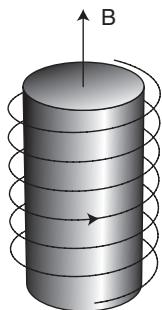
\includegraphics[width=0.34\textwidth]{figs/ch12/fig_12.16.jpg}
\caption*{图 12.16\quad 被磁线圈包围的圆柱形超导体。}\label{fig:auto:12.16}
\end{figure}

磁线圈中的电流由场 $H$ 保持恒定。因此，必然存在矢量场 $\mathbf A(\mathbf r)$ 与磁场产生的电流之间相互作用的贡献。安培定律给出
\begin{equation*}
\nabla\times\mathbf H=\frac{4\pi}{c}\mathbf J, \tag{12.204}
\end{equation*}
其中 $\mathbf J$ 是产生磁场的线圈中的电流。它对能量密度的贡献为
\begin{align*}
W&=-\int\mathbf A\cdot\frac{\nabla\times\mathbf H}{4\pi}\,\frac{\mathrm d\mathbf r}{V}\\
&=-\int\frac{\nabla\times\mathbf A}{4\pi}\cdot\mathbf H\,\frac{\mathrm d\mathbf r}{V}\\
&=-\int\mathbf B\cdot\mathbf H\,\frac{\mathrm d\mathbf r}{4\pi V}. \tag{12.205}
\end{align*}
在均匀系统中 $\mathbf B=\mathbf H$，场导致的总内能为 $H^2/8\pi-H^2/4\pi=-H^2/8\pi$。在正常态，这一能量必须计入总基态能量。因此，存在磁场时正常态的能量为 $E^0_{\mathrm n}=E'_{\mathrm n}-H^2/8\pi$。由于场不穿透超导体，超导体的内能保持 $E'_{\mathrm s}$ 不变。超导电性将持续到 $E'_{\mathrm n}-H^2/8\pi>E'_{\mathrm s}$ 为止。因此
\begin{equation*}
\frac{H^2}{8\pi}>E'_{\mathrm n}-E'_{\mathrm s}=-\delta E \tag{12.206}
\end{equation*}
是场的临界值的判据。我们发现，临界场
\begin{equation*}
H_{\mathrm c}=\sqrt{-8\pi\delta E}=\sqrt{4\pi N\left(\epsilon_{\mathrm F}-\mu\right)}\,\Delta, \tag{12.207}
\end{equation*}
正比于能隙参数 $\Delta$。

\section{能隙}

引入
\begin{align*}
\Delta_{\mathbf p}&=-\sum_{\mathbf p'}V_{\mathbf p\mathbf p'}u^*_{\mathbf p'}v_{\mathbf p'}\\
&=-\sum_{\mathbf p'}V_{\mathbf p\mathbf p'}\frac{\Delta_{\mathbf p'}}{2\varepsilon_{\mathbf p'}}, \tag{12.208}
\end{align*}
作为能隙的物理动机在于：这个量把连续的单粒子谱 $\epsilon_{\mathbf p}$ 劈裂成两支。专门针对只在费米能附近窄动量壳层内非零的模型势，我们把能隙方程改写为
\begin{equation*}
\Delta_{\mathbf p}=V_0{\sum_{\mathbf p'}}\frac{\Delta_{\mathbf p'}}{2\sqrt{\epsilon^2_{\mathbf p'}+\Delta^2_{\mathbf p'}}}. \tag{12.209}
\end{equation*}
求和上的撇号表示限制 $\left|\epsilon_{\mathbf p}-\epsilon_{\mathbf p_{\mathrm F}}\right|<\hbar\omega_{\mathrm D}$。在动量壳层内，只有当费米面各向同性时，$\Delta_{\mathbf p}$ 才相对地与 $\mathbf p$ 无关。对 $s$ 波配对，费米面完全各向同性，能隙可取为与 $\mathbf p$ 无关。对更高角动量的配对态（如 $d$ 波），费米面有节点，能隙的动量依赖不可忽略。为我们的目的，这里我们假定 $\Delta_{\mathbf p}$ 至少在费米面附近的薄动量壳层内与 $\mathbf p$ 无关。能隙方程的一个直接解是 $\Delta=0$。若 $\Delta=0$，则 $\langle b_{\mathbf p}\rangle=0$，从而只可能有正常相。

为得到能隙方程的非平凡解，我们把求和化为积分：
\begin{align*}
1&=N\left(\epsilon_{\mathrm F}-\mu\right)V_0\int_{-\hbar\omega_{\mathrm D}}^{\hbar\omega_{\mathrm D}}\frac{\mathrm d\epsilon}{2\sqrt{\epsilon^2+\Delta^2}}\\
&=N\left(\epsilon_{\mathrm F}-\mu\right)V_0\int_0^{\hbar\omega_{\mathrm D}/\Delta}\frac{\mathrm d\epsilon}{\sqrt{\epsilon^2+1}}\\
&=N\left(\epsilon_{\mathrm F}-\mu\right)V_0\sinh^{-1}\frac{\hbar\omega_{\mathrm D}}{\Delta}. \tag{12.210}
\end{align*}
因此，能隙由下式给出
\begin{equation*}
\Delta=\frac{\hbar\omega_{\mathrm D}}{\sinh\left(1/N\left(\epsilon_{\mathrm F}-\mu\right)V_0\right)}. \tag{12.211}
\end{equation*}
通常，$N\left(\epsilon_{\mathrm F}-\mu\right)V_0\ll 1$。在这个极限下，能隙取熟悉的形式
\begin{equation*}
\Delta(T=0)\simeq 2\hbar\omega_{\mathrm D}\exp\left(-\frac{1}{N(0)V_0}\right). \tag{12.212}
\end{equation*}
在库珀问题中，我们曾证明一个对的结合能与 $\Delta(T=0)$ 相同，只是 $1/\left(N(0)V_0\right)\to 2/\left(N(0)V_0\right)$。在完整理论中，如前所述，费米能以下粒子的配对也被包括进来。因此，精确的指数是 $2/\left(2N(0)V_0\right)=1/\left(N(0)V_0\right)$。在这个意义上，费米面以下粒子的配对有效地使费米能级处的态密度加倍。把能隙与 $T_{\mathrm c}$（式 (12.152)）比较，我们发现
\begin{equation*}
\frac{2\Delta}{k_{\mathrm B}T_{\mathrm c}}=\frac{4\hbar\omega_{\mathrm D}}{1.14\,\hbar\omega_{\mathrm D}}=3.52, \tag{12.213}
\end{equation*}
这是 BCS 理论中的关键比值。它决定超导体是否处于（相对于声子相互作用的）弱耦合极限。强耦合对应 $2\Delta/k_{\mathrm B}T_{\mathrm c}>3.5$。

为计算有限温度下的能隙，我们把费米分布权重因子 $1-n_{\mathbf p\uparrow}-n_{-\mathbf p\downarrow}$ 包括进来，它计及所有粒子之间的配对。因为 $n_{\mathbf p\uparrow}=n_{-\mathbf p\downarrow}$，我们可以把有限温能隙方程写成
\begin{equation*}
\Delta_{\mathbf p}=-\sum_{\mathbf p'}V_{\mathbf p\mathbf p'}\frac{\left(1-2n_{\mathbf p'}\right)}{2\varepsilon_{\mathbf p'}}\Delta_{\mathbf p'}. \tag{12.214}
\end{equation*}
对各向同性系统和 BCS 模型势，我们得到
\begin{equation*}
1=V_0N(0)\int_{-\hbar\omega_{\mathrm D}}^{\hbar\omega_{\mathrm D}}\frac{\tanh\beta\sqrt{\epsilon^2+\Delta^2}/2}{2\sqrt{\epsilon^2+\Delta^2}}\,\mathrm d\epsilon \tag{12.215}
\end{equation*}
作为激发谱中有限温能隙的定义方程。这个方程必须数值求解。不过，其近似解为 $\Delta(T)=\Delta(T=0)\sqrt{1-T/T_{\mathrm c}}$。这一行为如图 12.17 所示。

\begin{figure}[H]\centering
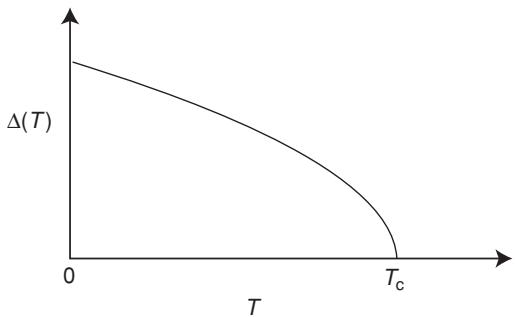
\includegraphics[width=0.5\textwidth]{figs/ch12/fig_12.17.jpg}
\caption*{图 12.17\quad 模型 BCS 相互作用下能隙的渐近行为。渐近地，能隙按 $\Delta(T)=\Delta(T=0)\left(1-\frac{T}{T_{\mathrm c}}\right)^{1/2}$ 标度。}\label{fig:auto:12.17}
\end{figure}

回忆序参量的二阶涨落
\begin{equation*}
\langle\delta\chi^2\rangle=-\frac{1}{V^2}\sum_{\mathbf p}u^{*2}_{\mathbf p}v^2_{\mathbf p}, \tag{12.216}
\end{equation*}正是由与能隙完全相同的相干因子组合决定的。由此我们立即看出，只要能隙行为良好，$\langle\delta\chi^{2}\rangle$ 在热力学极限下必为零。因此，$\langle b_{\mathbf{p}}\rangle$ 在超导态中取确定值。

\section{准粒子激发}

为了确定往超导体中添加一个额外粒子所需的能量，我们首先求出往 $|\Psi_{\mathrm{BCS}}\rangle$ 中添加一个额外电子的归一化产生算符。一开始我们便注意到
\begin{align*}
a_{\mathbf{p}'\uparrow}^{\dagger}|\Psi_{\mathrm{BCS}}\rangle&=a_{\mathbf{p}'\uparrow}^{\dagger}\prod_{\mathbf{p}}\left(u_{\mathbf{p}}+v_{\mathbf{p}}b_{\mathbf{p}}^{\dagger}\right)|0\rangle\\
&=a_{\mathbf{p}'\uparrow}^{\dagger}u_{\mathbf{p}'}\prod_{\mathbf{p}\neq\mathbf{p}'}\left(u_{\mathbf{p}}+v_{\mathbf{p}}b_{\mathbf{p}}^{\dagger}\right)|0\rangle\\
&=u_{\mathbf{p}'}|\psi_{\mathbf{p}'\uparrow}\rangle\tag{12.217}
\end{align*}
以及
\begin{align*}
a_{-\mathbf{p}'\downarrow}|\Psi_{\mathrm{BCS}}\rangle&=a_{-\mathbf{p}'\downarrow}v_{\mathbf{p}'}a_{\mathbf{p}'\uparrow}^{\dagger}a_{-\mathbf{p}'\downarrow}^{\dagger}\prod_{\mathbf{p}\neq\mathbf{p}'}\left(u_{\mathbf{p}}+v_{\mathbf{p}}b_{\mathbf{p}}^{\dagger}\right)|0\rangle\\
&=-v_{\mathbf{p}'}|\psi_{\mathbf{p}'\uparrow}\rangle,\tag{12.218}
\end{align*}
其中
\begin{equation*}
|\psi_{\mathbf{p}'\uparrow}\rangle=a_{\mathbf{p}'\uparrow}^{\dagger}\prod_{\mathbf{p}\neq\mathbf{p}'}\left(u_{\mathbf{p}}+v_{\mathbf{p}}b_{\mathbf{p}}^{\dagger}\right)|0\rangle\tag{12.219}
\end{equation*}
是在 BCS 基态中添加一个动量为 $\mathbf{p}$、自旋向上的额外电子之后所得的归一化波函数。因此，$a_{\mathbf{p}\uparrow}^{\dagger}$ 与 $a_{-\mathbf{p}\downarrow}$ 并非构造激发态所应使用的算符，因为所得的态未归一化。然而，电子算符的下述线性组合
\begin{equation*}
\gamma_{\mathbf{p}\uparrow}^{\dagger}=u_{\mathbf{p}}^{*}a_{\mathbf{p}\uparrow}^{\dagger}-v_{\mathbf{p}}^{*}a_{-\mathbf{p}\downarrow},\tag{12.220}
\end{equation*}
在作用于 $|\Psi_{\mathrm{BCS}}\rangle$ 时，
\begin{align*}
\gamma_{\mathbf{p}\uparrow}^{\dagger}|\Psi_{\mathrm{BCS}}\rangle&=\left(u_{\mathbf{p}}^{*}a_{\mathbf{p}\uparrow}^{\dagger}-v_{\mathbf{p}}^{*}a_{-\mathbf{p}\downarrow}\right)\prod_{\mathbf{p}'}\left(u_{\mathbf{p}'}+v_{\mathbf{p}'}b_{\mathbf{p}'}^{\dagger}\right)|0\rangle\\
&=\left(|u_{\mathbf{p}}|^{2}+|v_{\mathbf{p}}|^{2}\right)|\psi_{\mathbf{p}\uparrow}\rangle\\
&=|\psi_{\mathbf{p}\uparrow}\rangle\tag{12.221}
\end{align*}
的确产生归一化的态 $|\psi_{\mathbf{p}\uparrow}\rangle$。态 $|\psi_{-\mathbf{p}\downarrow}\rangle$ 相应的产生算符是
\begin{equation*}
\gamma_{-\mathbf{p}\downarrow}^{\dagger}=u_{\mathbf{p}}^{*}a_{-\mathbf{p}\downarrow}^{\dagger}+v_{\mathbf{p}}^{*}a_{\mathbf{p}\uparrow}.\tag{12.222}
\end{equation*}
由于诸 $\gamma_{\mathbf{p}}$ 是诸 $a_{\mathbf{p}}$ 的线性组合，它们必须服从标准的费米–狄拉克反对易关系，即
\begin{align*}
&\left[\gamma_{\mathbf{p}\sigma},\gamma_{\mathbf{p}'\sigma'}^{\dagger}\right]_{+}=\delta_{\mathbf{p}\mathbf{p}'}\delta_{\sigma\sigma'},\\
&\left[\gamma_{\mathbf{p}\sigma},\gamma_{\mathbf{p}'\sigma'}\right]_{+}=\left[\gamma_{\mathbf{p}\sigma}^{\dagger},\gamma_{\mathbf{p}'\sigma'}^{\dagger}\right]_{+}=0.\tag{12.223}
\end{align*}
反对易关系保证
\begin{equation*}
\gamma_{\mathbf{p}\uparrow}|\Psi_{\mathrm{BCS}}\rangle=\gamma_{-\mathbf{p}\downarrow}|\Psi_{\mathrm{BCS}}\rangle=0.\tag{12.224}
\end{equation*}
也就是说，超导体的基态中不存在准粒子。

由于诸 $\gamma_{\mathbf{p}}^{\dagger}$ 是自旋反平行的电子算符与空穴算符的线性组合，由这些算符产生的激发不携带确定的电荷。也就是说，在超导体中产生一个准粒子并不保证电荷守恒。不过，准粒子具有确定的自旋，因为添加一个自旋为 $\hbar/2$ 的电子或一个自旋为 $-\hbar/2$ 的空穴，都会产生 $S_{z}$ 的自旋为 $\hbar/2$ 的本征态。另一方面，库珀对携带电荷 $2e$，但在单态通道中无自旋。因此，在标准的单态 BCS 超导体中，携带确定自旋的量与携带确定电荷的量是彼此不同的实体。正是在这个意义上，单态 BCS 超导体中存在自旋–电荷分离。下面我们证明，单态超导体中自旋载体的能量色散关系是 $\varepsilon_{\mathbf{p}}$。为证明这一论断，我们从 $a_{\mathbf{p}\uparrow}$ 的运动方程出发：
\begin{align*}
\mathrm{i}\hbar\dot{a}_{\mathbf{p}\uparrow}&=\epsilon_{\mathbf{p}}a_{\mathbf{p}\uparrow}-\sum_{\mathbf{p}_{1},\mathbf{p}_{2}}V_{\mathbf{p}_{1}\mathbf{p}_{2}}\left[a_{\mathbf{p}\uparrow},b_{\mathbf{p}_{1}}^{\dagger}b_{\mathbf{p}_{2}}\right]\\
&=\epsilon_{\mathbf{p}}a_{\mathbf{p}\uparrow}+\sum_{\mathbf{p}_{1}}V_{\mathbf{p}\mathbf{p}_{1}}b_{\mathbf{p}_{1}}a_{-\mathbf{p}\downarrow}^{\dagger},\tag{12.225}
\end{align*}
以及 $a_{-\mathbf{p}\downarrow}^{\dagger}$ 的运动方程
\begin{equation*}
\mathrm{i}\hbar\dot{a}_{-\mathbf{p}\downarrow}^{\dagger}=-\epsilon_{\mathbf{p}}a_{-\mathbf{p}\downarrow}^{\dagger}+\sum_{\mathbf{p}_{2}}V_{\mathbf{p}\mathbf{p}_{2}}b_{\mathbf{p}_{2}}^{\dagger}a_{\mathbf{p}\uparrow}.\tag{12.226}
\end{equation*}
为简化这两个运动方程，我们把 $\sum_{\mathbf{p}_{1}}V_{\mathbf{p}\mathbf{p}_{1}}b_{\mathbf{p}_{1}}$ 替换为它的平均值：$-\Delta_{\mathbf{p}}=\sum_{\mathbf{p}_{1}}V_{\mathbf{p}\mathbf{p}_{1}}\langle b_{\mathbf{p}_{1}}\rangle$。于是，有效哈密顿量
\begin{equation*}
H_{\mathrm{eff}}=\sum_{\mathbf{p}\sigma}\epsilon_{\mathbf{p}}n_{\mathbf{p}\sigma}-\sum_{\mathbf{p}}\Delta_{\mathbf{p}}\left(b_{\mathbf{p}}^{\dagger}+b_{\mathbf{p}}\right)\tag{12.227}
\end{equation*}
对配对算符 $b_{\mathbf{p}}^{\dagger}$ 是线性的，不同于完整哈密顿量中的二次型。其结果是，在约化哈密顿量中粒子数不再守恒。尽管如此，BCS 哈密顿量的平均场处理仍然给出超导态的准确描述。这种局面之所以出现，部分原因在于 BCS 基态并不具有固定的粒子数。

平均场闭合导致一组耦合方程：
\begin{align*}
&\mathrm{i}\hbar\dot{a}_{\mathbf{p}\uparrow}=\epsilon_{\mathbf{p}}a_{\mathbf{p}\uparrow}-\Delta_{\mathbf{p}}a_{-\mathbf{p}\downarrow}^{\dagger},\\
&\mathrm{i}\hbar\dot{a}_{-\mathbf{p}\downarrow}^{\dagger}=-\epsilon_{\mathbf{p}}a_{-\mathbf{p}\downarrow}^{\dagger}-\Delta_{\mathbf{p}}a_{\mathbf{p}\uparrow},\tag{12.228}
\end{align*}
它们对能隙参量 $\Delta_{\mathbf{p}}$ 是线性的。为记号简洁，我们把这组方程改写成矩阵形式：
\begin{align*}
\mathrm{i}\hbar\frac{\partial}{\partial t}\begin{pmatrix}a_{\mathbf{p}\uparrow}\\ a_{-\mathbf{p}\downarrow}^{\dagger}\end{pmatrix}&=\begin{pmatrix}\epsilon_{\mathbf{p}} & -\Delta_{\mathbf{p}}\\ -\Delta_{\mathbf{p}} & -\epsilon_{\mathbf{p}}\end{pmatrix}\begin{pmatrix}a_{\mathbf{p}\uparrow}\\ a_{-\mathbf{p}\downarrow}^{\dagger}\end{pmatrix}\\
&=\mathbf{H}_{\mathrm{eff}}\begin{pmatrix}a_{\mathbf{p}\uparrow}\\ a_{-\mathbf{p}\downarrow}^{\dagger}\end{pmatrix}.\tag{12.229}
\end{align*}
为帮助把约化哈密顿量矩阵对角化，我们引入角度 $\theta_{\mathbf{p}}$，使得
\begin{equation*}
\cos\theta_{\mathbf{p}}=\frac{\epsilon_{\mathbf{p}}}{\varepsilon_{\mathbf{p}}}\tag{12.230}
\end{equation*}
以及
\begin{equation*}
\sin\theta_{\mathbf{p}}=\frac{\Delta_{\mathbf{p}}}{\varepsilon_{\mathbf{p}}}.\tag{12.231}
\end{equation*}
这一变换的用处立竿见影，因为 BCS 系数
\begin{equation*}
u_{\mathbf{p}}=\frac{1}{\sqrt{2}}\left(1+\frac{\epsilon_{\mathbf{p}}}{\varepsilon_{\mathbf{p}}}\right)^{1/2}=\frac{1}{\sqrt{2}}\left(1+\cos\theta_{\mathbf{p}}\right)^{1/2}\tag{12.232}
\end{equation*}
与
\begin{equation*}
v_{\mathbf{p}}=\frac{1}{\sqrt{2}}\left(1-\frac{\epsilon_{\mathbf{p}}}{\varepsilon_{\mathbf{p}}}\right)^{1/2}=\frac{1}{\sqrt{2}}\left(1-\cos\theta_{\mathbf{p}}\right)^{1/2}\tag{12.233}
\end{equation*}
构成约化哈密顿量矩阵的本征矢基底，
\begin{equation*}
\mathbf{H}_{\mathrm{eff}}=\varepsilon_{\mathbf{p}}\begin{pmatrix}\cos\theta_{\mathbf{p}} & -\sin\theta_{\mathbf{p}}\\ -\sin\theta_{\mathbf{p}} & -\cos\theta_{\mathbf{p}}\end{pmatrix}.\tag{12.234}
\end{equation*}
该矩阵的本征值是 $\pm 1$。因此，本征矢形如
\begin{equation*}
\begin{pmatrix}\sin\theta_{\mathbf{p}}\\ \cos\theta_{\mathbf{p}}\pm 1\end{pmatrix}.\tag{12.235}
\end{equation*}
本征矢中两组系数之比为
\begin{equation*}
\frac{\sin\theta_{\mathbf{p}}}{(\cos\theta_{\mathbf{p}}\pm 1)}=\pm\left(\tan\frac{\theta_{\mathbf{p}}}{2}\right)^{\pm 1}.\tag{12.236}
\end{equation*}
由于
\begin{equation*}
\tan\frac{\theta_{\mathbf{p}}}{2}=\pm\left(\frac{\sqrt{1-\cos\theta_{\mathbf{p}}}}{\sqrt{1+\cos\theta_{\mathbf{p}}}}\right),\tag{12.237}
\end{equation*}
$\mathbf{H}_{\mathrm{eff}}$ 的本征矢可以写成
\begin{equation*}
\mathbf{e}_{1}=\begin{pmatrix}v_{\mathbf{p}}\\ u_{\mathbf{p}}\end{pmatrix}=\begin{pmatrix}\sin\left(\theta_{\mathbf{p}}/2\right)\\ \cos\left(\theta_{\mathbf{p}}/2\right)\end{pmatrix}\tag{12.238}
\end{equation*}
以及
\begin{equation*}
\mathbf{e}_{2}=\begin{pmatrix}u_{\mathbf{p}}\\ -v_{\mathbf{p}}\end{pmatrix}=\begin{pmatrix}\cos\left(\theta_{\mathbf{p}}/2\right)\\ -\sin\left(\theta_{\mathbf{p}}/2\right)\end{pmatrix}.\tag{12.239}
\end{equation*}
现在可以清楚地看到 $\mathbf{H}_{\mathrm{eff}}\mathbf{e}_{1}=-\varepsilon_{\mathbf{p}}\mathbf{e}_{1}$ 且 $\mathbf{H}_{\mathrm{eff}}\mathbf{e}_{2}=\varepsilon_{\mathbf{p}}\mathbf{e}_{2}$。简言之，$\pm\varepsilon_{\mathbf{p}}$ 是 $\mathbf{H}_{\mathrm{eff}}$ 的两个本征能量。为阐明 $\mathbf{e}_{1}$ 与 $\mathbf{e}_{2}$ 的用处，我们用 $\mathbf{e}_{1}$ 和 $\mathbf{e}_{2}$ 去乘运动方程。对 $\mathbf{e}_{2}$ 的结果
\begin{align*}
\mathrm{i}\hbar\frac{\partial}{\partial t}\left(a_{\mathbf{p}\uparrow}u_{\mathbf{p}}-v_{\mathbf{p}}a_{-\mathbf{p}\downarrow}^{\dagger}\right)&=\mathbf{e}_{2}^{\mathrm{T}}\mathbf{H}_{\mathrm{eff}}\begin{pmatrix}a_{\mathbf{p}\uparrow}\\ a_{-\mathbf{p}\downarrow}^{\dagger}\end{pmatrix}\\
&=\varepsilon_{\mathbf{p}}\mathbf{e}_{2}^{\mathrm{T}}\begin{pmatrix}a_{\mathbf{p}\uparrow}\\ a_{-\mathbf{p}\downarrow}^{\dagger}\end{pmatrix},\tag{12.240}
\end{align*}
表明
\begin{equation*}
\mathrm{i}\hbar\dot{\gamma}_{\mathbf{p}\uparrow}=\varepsilon_{\mathbf{p}}\gamma_{\mathbf{p}\uparrow}.\tag{12.241}
\end{equation*}
类似地，对 $\mathbf{e}_{1}$ 有
\begin{equation*}
\mathrm{i}\hbar\frac{\partial}{\partial t}\left(v_{\mathbf{p}}^{*}a_{\mathbf{p}\uparrow}+u_{\mathbf{p}}^{*}a_{-\mathbf{p}\downarrow}^{\dagger}\right)=-\varepsilon_{\mathbf{p}}\mathbf{e}_{1}^{\dagger}\begin{pmatrix}a_{\mathbf{p}\uparrow}\\ a_{-\mathbf{p}\downarrow}^{\dagger}\end{pmatrix}\tag{12.242}
\end{equation*}
以及
\begin{equation*}
\mathrm{i}\hbar\dot{\gamma}_{-\mathbf{p}\downarrow}^{\dagger}=-\varepsilon_{\mathbf{p}}\gamma_{-\mathbf{p}\downarrow}^{\dagger}.\tag{12.243}
\end{equation*}
这些运动方程意味着约化哈密顿量对角化后的形式为
\begin{equation*}
\mathbf{H}_{\mathrm{eff}}=\sum_{\mathbf{p}}\varepsilon_{\mathbf{p}}\left(\gamma_{\mathbf{p}\uparrow}^{\dagger}\gamma_{\mathbf{p}\uparrow}+\gamma_{-\mathbf{p}\downarrow}^{\dagger}\gamma_{-\mathbf{p}\downarrow}\right).\tag{12.244}
\end{equation*}

\begin{figure}[H]\centering
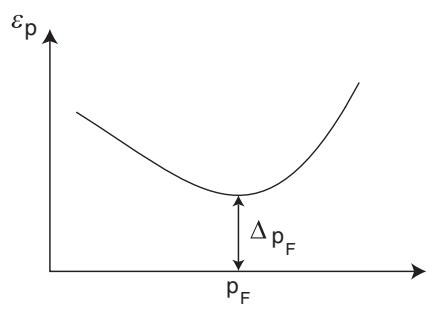
\includegraphics[width=0.44\textwidth]{figs/ch12/fig_12.18_a.jpg}\hfill
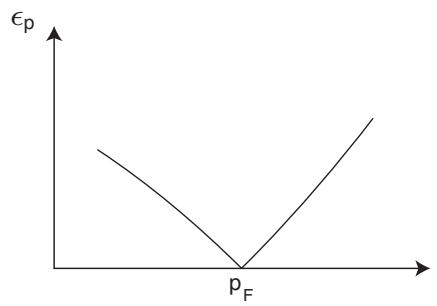
\includegraphics[width=0.44\textwidth]{figs/ch12/fig_12.18_b.jpg}
\caption*{图 12.18\quad (a) 超导态与 (b) 正常态下费米面附近的准粒子谱。$\epsilon_{\mathbf{p}}$ 在费米能级处的取值选定为零。因此，费米面处所需的最小激发能就是能隙能量。}\label{fig:auto:12.18}
\end{figure}

因此，产生任何准粒子，无论其自旋与动量如何，都需要花费能量 $\varepsilon_{\mathbf{p}}$。再强调一遍，BCS 理论的准粒子并不是电子；它们是有自旋但无确定电荷的实体，这与携带电荷 $2e$ 却无自旋的单态库珀对恰成对照。在这个意义上，可以认为 BCS 超导体中存在自旋–电荷分离。准粒子能量的图像示于图 12.18。显然，添加或移除一个粒子至少要花费最小能量 $\Delta_{\mathbf{p}}$。

\section{热力学}

我们现在可以着手计算超导体的热力学性质了。特别有意义的是热容 $C_{\mathrm{v}}$ 与亥姆霍兹自由能，前者在正常态与超导态之间存在不连续。为计算这些量，我们需要把运动方程表述成便于提取有限温度信息的形式。最便捷的做法是用准粒子算符重写模型哈密顿量。为此，我们把准粒子算符反解出来，用它们表示电子算符：
\begin{equation*}
a_{\mathbf{p}\uparrow}=u_{\mathbf{p}}^{*}\gamma_{\mathbf{p}\uparrow}+v_{\mathbf{p}}\gamma_{-\mathbf{p}\downarrow}^{\dagger}\tag{12.245}
\end{equation*}
以及
\begin{equation*}
a_{-\mathbf{p}\downarrow}=-v_{\mathbf{p}}\gamma_{\mathbf{p}\uparrow}^{\dagger}+u_{\mathbf{p}}^{*}\gamma_{-\mathbf{p}\downarrow}.\tag{12.246}
\end{equation*}
我们将证明，热平均
\begin{equation*}
\langle\gamma_{\mathbf{p}\sigma}^{\dagger}\gamma_{\mathbf{p}\sigma}\rangle=n_{\mathbf{p}\sigma},\tag{12.247}
\end{equation*}
其中 $n_{\mathbf{p}\sigma}$ 是在准粒子能量 $\varepsilon_{\mathbf{p}}$ 处取值的费米–狄拉克分布函数。我们将假定与这类准粒子激发相联系的熵由第 2 章给出的无相互作用形式
\begin{equation*}
S=-k_{\mathrm{B}}\sum_{\mathbf{p},\sigma}\left[n_{\mathbf{p}\sigma}\ln n_{\mathbf{p}\sigma}+\left(1-n_{\mathbf{p}\sigma}\right)\ln\left(1-n_{\mathbf{p}\sigma}\right)\right]\tag{12.248}
\end{equation*}
给出。与式 (12.244) 相结合，费米–狄拉克分布便必然成立。尽管如此，我们仍将显式地建立这一结果。

我们先计算亥姆霍兹自由能 $F=E'-TS$，其中 $E'=\langle H-\mu N\rangle$。需要在平均场层次上把内能
\begin{equation*}
E'=\sum_{\mathbf{p},\sigma}\epsilon_{\mathbf{p}}\langle a_{\mathbf{p}\sigma}^{\dagger}a_{\mathbf{p}\sigma}\rangle+\sum_{\mathbf{p},\mathbf{p}'}V_{\mathbf{p}\mathbf{p}'}\langle b_{\mathbf{p}}^{\dagger}\rangle\langle b_{\mathbf{p}'}\rangle,\tag{12.249}
\end{equation*}
用诸 $\gamma_{\mathbf{p}}$ 表示出来。这些表达式中的热平均应理解为对系统所有态的求迹。基态之上的一个任意激发态表示为
\begin{equation*}
|\text{激发态}\rangle=\prod_{i}\gamma_{\mathbf{p}_{i}\sigma_{i}}^{\dagger}|\Psi_{\mathrm{BCS}}\rangle\tag{12.250}
\end{equation*}
因而含有确定数目的被激发准粒子。于是，任何 $\langle\gamma\gamma\rangle$ 形式的平均恒等于零。由式 (12.245) 与式 (12.246) 可得
\begin{align*}
\sum_{\mathbf{p},\sigma}\langle a_{\mathbf{p}\sigma}^{\dagger}a_{\mathbf{p}\sigma}\rangle&=\sum_{\mathbf{p}}\Big\langle\big(u_{\mathbf{p}}\gamma_{\mathbf{p}\uparrow}^{\dagger}+v_{\mathbf{p}}^{*}\gamma_{-\mathbf{p}\downarrow}\big)\big(u_{\mathbf{p}}^{*}\gamma_{\mathbf{p}\uparrow}+v_{\mathbf{p}}\gamma_{-\mathbf{p}\downarrow}^{\dagger}\big)\Big\rangle\\
&\quad+\sum_{\mathbf{p}}\Big\langle\big(-v_{\mathbf{p}}^{*}\gamma_{\mathbf{p}\uparrow}+u_{\mathbf{p}}\gamma_{-\mathbf{p}\downarrow}^{\dagger}\big)\big(-v_{\mathbf{p}}\gamma_{\mathbf{p}\uparrow}^{\dagger}+u_{\mathbf{p}}^{*}\gamma_{-\mathbf{p}\downarrow}\big)\Big\rangle\\
&=\sum_{\mathbf{p}}\left(\left|u_{\mathbf{p}}\right|^{2}-\left|v_{\mathbf{p}}\right|^{2}\right)\left(n_{\mathbf{p}\uparrow}+n_{-\mathbf{p}\downarrow}\right)+2\left|v_{\mathbf{p}}\right|^{2}.\tag{12.251}
\end{align*}
在基态中，我们前面已经证明（见式 (12.171)）$\langle b_{\mathbf{p}}\rangle=u_{\mathbf{p}}^{*}v_{\mathbf{p}}$。有限温度下，配对算符的平均值
\begin{align*}
\langle b_{\mathbf{p}}\rangle&=\langle a_{-\mathbf{p}\downarrow}a_{\mathbf{p}\uparrow}\rangle=\Big\langle\big(-v_{\mathbf{p}}\gamma_{\mathbf{p}\uparrow}^{\dagger}+u_{\mathbf{p}}^{*}\gamma_{-\mathbf{p}\downarrow}\big)\big(u_{\mathbf{p}}^{*}\gamma_{\mathbf{p}\uparrow}+v_{\mathbf{p}}\gamma_{-\mathbf{p}\downarrow}^{\dagger}\big)\Big\rangle\\
&=v_{\mathbf{p}}u_{\mathbf{p}}^{*}\left(1-n_{-\mathbf{p}\downarrow}-n_{\mathbf{p}\uparrow}\right)\tag{12.252}
\end{align*}
包含反映费米能级上下电子配对的热因子。因此，
\begin{equation*}
\sum_{\mathbf{p},\mathbf{p}'}V_{\mathbf{p}\mathbf{p}'}\langle b_{\mathbf{p}}^{\dagger}\rangle\langle b_{\mathbf{p}'}\rangle=\sum_{\mathbf{p},\mathbf{p}'}V_{\mathbf{p}\mathbf{p}'}\,u_{\mathbf{p}}u_{\mathbf{p}'}^{*}v_{\mathbf{p}}^{*}v_{\mathbf{p}'}\left(1-n_{\mathbf{p}\uparrow}-n_{-\mathbf{p}\downarrow}\right)\left(1-n_{-\mathbf{p}'\downarrow}-n_{\mathbf{p}'\uparrow}\right),\tag{12.253}
\end{equation*}
总的亥姆霍兹能量即为
\begin{align*}
F'&=\sum_{\mathbf{p}}\epsilon_{\mathbf{p}}\left[\left(\left|u_{\mathbf{p}}\right|^{2}-\left|v_{\mathbf{p}}\right|^{2}\right)\left(n_{\mathbf{p}\uparrow}+n_{-\mathbf{p}\downarrow}\right)+2\left|v_{\mathbf{p}}\right|^{2}\right]\\
&\quad+\sum_{\mathbf{p},\mathbf{p}'}V_{\mathbf{p}\mathbf{p}'}\left(1-n_{-\mathbf{p}\downarrow}-n_{\mathbf{p}\uparrow}\right)\left(1-n_{-\mathbf{p}'\downarrow}-n_{\mathbf{p}'\uparrow}\right)u_{\mathbf{p}}v_{\mathbf{p}}^{*}u_{\mathbf{p}'}^{*}v_{\mathbf{p}'}\\
&\quad+k_{\mathrm{B}}T\sum_{\mathbf{p},\sigma}\left[n_{\mathbf{p}\sigma}\ln n_{\mathbf{p}\sigma}+\left(1-n_{\mathbf{p}\sigma}\right)\ln\left(1-n_{\mathbf{p}\sigma}\right)\right].\tag{12.254}
\end{align*}
对 $u_{\mathbf{p}}$ 与 $v_{\mathbf{p}}$ 求 $F'$ 的极小，得到标准结果 $u_{\mathbf{p}}=\left(\left(1+\cos\theta_{\mathbf{p}}\right)/2\right)^{1/2}$ 与 $v_{\mathbf{p}}=\left(\left(1-\cos\theta_{\mathbf{p}}\right)/2\right)^{1/2}$，且 $\cos\theta_{\mathbf{p}}=\epsilon_{\mathbf{p}}/\varepsilon_{\mathbf{p}}$。但在这种情形下，能隙通过
\begin{align*}
\Delta_{\mathbf{p}}&=-\sum_{\mathbf{p}'}V_{\mathbf{p}\mathbf{p}'}\langle b_{\mathbf{p}'}\rangle\\
&=-\sum_{\mathbf{p}'}V_{\mathbf{p}\mathbf{p}'}\left(1-n_{\mathbf{p}'\uparrow}-n_{-\mathbf{p}'\downarrow}\right)u_{\mathbf{p}'}^{*}v_{\mathbf{p}'},\tag{12.255}
\end{align*}
依赖于温度，其中 $\sin\theta_{\mathbf{p}}=\Delta_{\mathbf{p}}/\varepsilon_{\mathbf{p}}$。对 $n_{\mathbf{p}\uparrow}$ 变分 $F'$，我们得到
\begin{equation*}
\frac{\partial F'}{\partial n_{\mathbf{p}\uparrow}}=0=\epsilon_{\mathbf{p}}\left(\left|u_{\mathbf{p}}\right|^{2}-\left|v_{\mathbf{p}}\right|^{2}\right)+k_{\mathrm{B}}T\ln\left(\frac{n_{\mathbf{p}\uparrow}}{1-n_{\mathbf{p}\uparrow}}\right)+2\Delta_{\mathbf{p}}u_{\mathbf{p}}v_{\mathbf{p}}^{*},\tag{12.256}
\end{equation*}
其中相干因子 $u_{\mathbf{p}}$ 与 $v_{\mathbf{p}}$ 保持固定。此时加在 $n_{\mathbf{p}\uparrow}$ 上的条件，即
\begin{align*}
k_{\mathrm{B}}T\ln\left(n_{\mathbf{p}\uparrow}^{-1}-1\right)&=\epsilon_{\mathbf{p}}\cos\theta_{\mathbf{p}}+2\Delta_{\mathbf{p}}u_{\mathbf{p}}v_{\mathbf{p}}^{*}\\
&=\epsilon_{\mathbf{p}}\cos\theta_{\mathbf{p}}+\Delta_{\mathbf{p}}\sin\theta_{\mathbf{p}}\\
&=\varepsilon_{\mathbf{p}},\tag{12.257}
\end{align*}
不过是要求 $n_{\mathbf{p}\uparrow}$ 为在准能量 $\varepsilon_{\mathbf{p}}$ 处取值的费米–狄拉克分布。费米–狄拉克分布是有限温度下准粒子激发的最概然分布。

若采用能隙的平均场值，即式 (12.255)，自由能的计算便直截了当：
\begin{align*}
E'&=\sum_{\mathbf{p}}\epsilon_{\mathbf{p}}\left[\left(\left|u_{\mathbf{p}}\right|^{2}-\left|v_{\mathbf{p}}\right|^{2}\right)\left(n_{\mathbf{p}\uparrow}+n_{\mathbf{p}\downarrow}\right)+2\left|v_{\mathbf{p}}\right|^{2}\right]-\sum_{\mathbf{p}}\Delta_{\mathbf{p}}\frac{\sin\theta_{\mathbf{p}}}{2}\left(1-2n_{\mathbf{p}}\right)\\
&=\sum_{\mathbf{p}}\left[2\epsilon_{\mathbf{p}}\left(\cos\theta_{\mathbf{p}}n_{\mathbf{p}}+\sin^{2}\frac{\theta_{\mathbf{p}}}{2}\right)-\Delta_{\mathbf{p}}\frac{\sin\theta_{\mathbf{p}}}{2}\left(1-2n_{\mathbf{p}}\right)\right].\tag{12.258}
\end{align*}
结合 $\ln\left(1/n_{\mathbf{p}\sigma}-1\right)=\varepsilon_{\mathbf{p}}/k_{\mathrm{B}}T$ 这一事实，我们把熵项简化为
\begin{equation*}
TS=-2k_{\mathrm{B}}T\sum_{\mathbf{p}}\left[\beta\varepsilon_{\mathbf{p}}n_{\mathbf{p}}+\ln\left(1+\mathrm{e}^{-\beta\varepsilon_{\mathbf{p}}}\right)\right].\tag{12.259}
\end{equation*}
总自由能即为
\begin{align*}
F'&=\sum_{\mathbf{p}}\left[2\epsilon_{\mathbf{p}}\left(\cos\theta_{\mathbf{p}}n_{\mathbf{p}}+\sin^{2}\frac{\theta_{\mathbf{p}}}{2}\right)-\Delta_{\mathbf{p}}\frac{\sin\theta_{\mathbf{p}}}{2}\left(1-2n_{\mathbf{p}}\right)\right]\\
&\quad+2k_{\mathrm{B}}T\sum_{\mathbf{p}}\left[\beta\varepsilon_{\mathbf{p}}n_{\mathbf{p}}+\ln\left(1+\mathrm{e}^{-\beta\varepsilon_{\mathbf{p}}}\right)\right].\tag{12.260}
\end{align*}
这一表达式的求值留作课后习题（见习题 12.10）。热容
\begin{align*}
C_{\mathrm{v}}&=T\left(\frac{\partial S}{\partial T}\right)_{V}\\
&=-k_{\mathrm{B}}T\sum_{\mathbf{p},\sigma}\frac{\partial n_{\mathbf{p}\sigma}}{\partial T}\ln\left(\frac{n_{\mathbf{p}\sigma}}{1-n_{\mathbf{p}\sigma}}\right)\\
&=\sum_{\mathbf{p},\sigma}\varepsilon_{\mathbf{p}}\frac{\partial n_{\mathbf{p}\sigma}}{\partial T},\tag{12.261}
\end{align*}
包含温度导数
\begin{equation*}
\frac{\partial n_{\mathbf{p}}}{\partial T}=\frac{n_{\mathbf{p}}^{2}}{k_{\mathrm{B}}T}\left[\frac{\varepsilon_{\mathbf{p}}}{T}-\frac{\partial\varepsilon_{\mathbf{p}}}{\partial T}\right]\mathrm{e}^{\beta\varepsilon_{\mathbf{p}}},\tag{12.262}
\end{equation*}
其中又叠加了能隙 $\Delta_{\mathbf{p}}$ 的隐式温度依赖。由 $\varepsilon_{\mathbf{p}}$ 的定义可得
\begin{equation*}
\frac{\partial\varepsilon_{\mathbf{p}}}{\partial T}=\frac{\partial\varepsilon_{\mathbf{p}}}{\partial\Delta_{\mathbf{p}}}\frac{\partial\Delta_{\mathbf{p}}}{\partial T}=\frac{\Delta_{\mathbf{p}}}{\varepsilon_{\mathbf{p}}}\frac{\partial\Delta_{\mathbf{p}}}{\partial T}=\frac{1}{2\varepsilon_{\mathbf{p}}}\frac{\partial\Delta_{\mathbf{p}}^{2}}{\partial T}.\tag{12.263}
\end{equation*}
由于 $\partial\varepsilon_{\mathbf{p}}/\partial T$ 在正常态中为零，我们把 $T=T_{\mathrm{c}}$ 处超导态与正常态热容之差写成
\begin{align*}
\left(C_{\mathrm{v}}^{\mathrm{S}}-C_{\mathrm{v}}^{\mathrm{N}}\right)_{T=T_{\mathrm{c}}}&=-\beta\sum_{\mathbf{p}}n_{\mathbf{p}}^{2}\frac{\partial\Delta_{\mathbf{p}}^{2}}{\partial T}\mathrm{e}^{\beta\varepsilon_{\mathbf{p}}}\\
&=\sum_{\mathbf{p}}\left.\frac{\partial n_{\mathbf{p}}}{\partial\varepsilon_{\mathbf{p}}}\frac{\partial\Delta_{\mathbf{p}}^{2}}{\partial T}\right|_{T=T_{\mathrm{c}}}.\tag{12.264}
\end{align*}
在 $T=T_{\mathrm{c}}$ 附近，能隙很好地近似为 $\Delta^{2}\sim|1-T/T_{\mathrm{c}}|$。于是我们发现 $\partial\Delta^{2}/\partial T\sim 1/T_{\mathrm{c}}$，而热容的不连续严格等于
\begin{equation*}
C_{\mathrm{v}}^{\mathrm{S}}-C_{\mathrm{v}}^{\mathrm{N}}=\frac{N(\epsilon_{\mathrm{F}})}{T_{\mathrm{c}}}\tag{12.265}
\end{equation*}
（在 $T=T_{\mathrm{c}}$ 处）。与这一差值相联系的正号表明，恰在 $T_{\mathrm{c}}$ 下方超导态的热容超过 $C_{\mathrm{v}}^{\mathrm{N}}$。

我们要寻找的第二个结果，是 $C_{\mathrm{v}}^{\mathrm{S}}$ 在 $T_{\mathrm{c}}$ 下方不远处的指数式衰减。为得到这一行为，我们在 $T\to 0$ 的极限下分析式 (12.261)。此极限下 $\partial\Delta_{\mathbf{p}}^{2}/\partial T\to 0$，$n_{\mathbf{p}}\to\mathrm{e}^{-\beta\varepsilon_{\mathbf{p}}}$，热容由下式主导：
\begin{align*}
\lim_{T\to 0}C_{\mathrm{v}}&=2\beta^{2}k_{\mathrm{B}}\sum_{\mathbf{p}}\varepsilon_{\mathbf{p}}^{2}n_{\mathbf{p}}\left(1-n_{\mathbf{p}}\right)\\
&\simeq 2\beta^{2}k_{\mathrm{B}}N(\epsilon_{\mathrm{F}})\Delta^{2}(T=0)\int_{0}^{\infty}\mathrm{d}\epsilon\,\mathrm{e}^{-\beta\sqrt{\Delta^{2}(T=0)+\epsilon^{2}}}\\
&\simeq 2\beta^{2}k_{\mathrm{B}}N(\epsilon_{\mathrm{F}})\Delta_{0}^{2}\mathrm{e}^{-\beta\Delta_{0}}\int_{0}^{\infty}\mathrm{d}\epsilon\,\mathrm{e}^{-\beta\epsilon^{2}/2\Delta_{0}}\\
&=N(\epsilon_{\mathrm{F}})\sqrt{\frac{\pi}{2}}\,k_{\mathrm{B}}\beta^{3/2}\Delta_{0}^{5/2}\mathrm{e}^{-\beta\Delta_{0}},\tag{12.266}
\end{align*}
如前所述，它按指数规律衰减，其中 $\Delta_{0}=\Delta(T=0)$。指数衰减由 $T=0$ 处的能隙主导。在简化导出这一结果的积分时，我们利用了积分在 $\Delta\gg\epsilon$ 时最大这一事实。

\section{实验应用}

BCS 理论的一项关键成功，是声子衰减率这类物理观测量可以十分便捷地计算出来。事实上，正是利用 BCS 理论完成的自旋–晶格弛豫时间计算及其随后的实验证实，才促成了 BCS 理论的广泛接受。本节我们显式地完成其中的三个计算：（1）电磁吸收；（2）超声衰减；（3）自旋–晶格弛豫速率。出现在每个计算中的，是相干因子 $u_{\mathbf{p}}$ 与 $v_{\mathbf{p}}$ 的特定组合。我们将会看到，相干因子的每一种组合都能产生完全不同的物理。物理性质与相干因子如此紧密相连，正是 BCS 配对假设的一个标志。在每个计算中，我们都把相干因子当作实数处理。如前所见，对我们所选的简单模型势，即式 (12.41)，相干因子实际上是实的。

\subsection{电磁吸收}

在 BCS 超导体中，频率低于 $\Delta/\hbar$ 的电磁辐射吸收受到抑制。现在我们拥有了显式导出这一结果的工具。在电磁问题中，微扰项通过把动量替换为 $\mathbf{p}-e\mathbf{A}(\mathbf{r},t)/c$ 得到，其中 $\mathbf{A}(\mathbf{r},t)$ 是矢势。准确到 $\mathbf{A}(\mathbf{r},t)$ 的最低阶，微扰具有 $\mathbf{p}\cdot\mathbf{A}+\mathbf{A}\cdot\mathbf{p}$ 的形式。我们将要求矢势满足横向条件 $\nabla\cdot\mathbf{A}=0$。于是，频率为 $\omega_{\mathbf{q}}$ 的电磁波被吸收时微扰的二次量子化形式为
\begin{equation*}
H_{\mathrm{abs}}=-\frac{e}{mcV}\sum_{\mathbf{p},\sigma}\mathbf{A}\cdot\mathbf{p}\,a_{\mathbf{p}+\mathbf{q}\sigma}^{\dagger}a_{\mathbf{p}\sigma}.\tag{12.267}
\end{equation*}

\begin{figure}[H]\centering
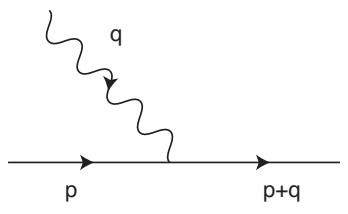
\includegraphics[width=0.44\textwidth]{figs/ch12/fig_12.19_a.jpg}\hfill
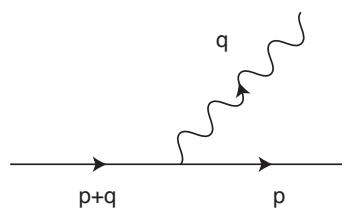
\includegraphics[width=0.44\textwidth]{figs/ch12/fig_12.19_b.jpg}\\[6pt]
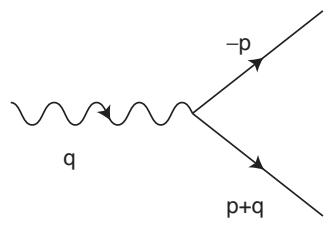
\includegraphics[width=0.5\textwidth]{figs/ch12/fig_12.19_c.jpg}
\caption*{图 12.19\quad 由电磁吸收矩阵元产生的准粒子激发：(a) $\gamma_{\mathbf{p}+\mathbf{q}}^{\dagger}\gamma_{\mathbf{p}}$，(b) $\gamma_{\mathbf{p}}^{\dagger}\gamma_{\mathbf{p}+\mathbf{q}}$，以及 (c) $\gamma_{\mathbf{p}+\mathbf{q}}^{\dagger}\gamma_{-\mathbf{p}}^{\dagger}$。波浪线表示光子相互作用。}\label{fig:auto:12.19}
\end{figure}

我们必须计算形如
\begin{equation*}
\langle f|H_{\mathrm{abs}}|i\rangle=-\frac{e}{mcV}\sum_{\mathbf{p}\sigma}\mathbf{A}\cdot\mathbf{p}\,M_{\mathrm{if}}^{\sigma},\tag{12.268}
\end{equation*}
的矩阵元，其中
\begin{equation*}
M_{\mathrm{if}}^{\sigma}=\langle f|a_{\mathbf{p}+\mathbf{q}\sigma}^{\dagger}a_{\mathbf{p}\sigma}|i\rangle\tag{12.269}
\end{equation*}
而 $|i\rangle$ 与 $|f\rangle$ 分别是初态与末态准粒子态。与热容的计算一样，我们把这个矩阵元
\begin{align*}
\sum_{\sigma}M_{\mathrm{if}}^{\sigma}&=\Big\langle f\Big|\big(u_{\mathbf{p}'}\gamma_{\mathbf{p}'\uparrow}^{\dagger}+v_{\mathbf{p}'}\gamma_{-\mathbf{p}'\downarrow}\big)\big(u_{\mathbf{p}}\gamma_{\mathbf{p}\uparrow}+v_{\mathbf{p}}\gamma_{-\mathbf{p}\downarrow}^{\dagger}\big)\Big|i\Big\rangle\\
&\quad+\Big\langle f\Big|\big(-v_{-\mathbf{p}'}\gamma_{-\mathbf{p}'\uparrow}+u_{-\mathbf{p}'}\gamma_{\mathbf{p}'\downarrow}^{\dagger}\big)\big(-v_{-\mathbf{p}}\gamma_{-\mathbf{p}\uparrow}^{\dagger}+u_{-\mathbf{p}}\gamma_{\mathbf{p}\downarrow}\big)\Big|i\Big\rangle,
\end{align*}
用准粒子算符改写。由上式产生若干种不同的准粒子激发，它们绘于图 12.19 中。

$T=0$ 时基态中没有准粒子。因此，图 12.19 所示的最后一个过程——即产生两个准粒子的过程——是 $T=0$ 下唯一存活的过程。我们就专门考虑 $T=0$ 的情形，因为此时本质物理最易揭示。我们得到
\begin{equation*}
M_{\mathrm{if}}^{\uparrow}+M_{\mathrm{if}}^{\downarrow}=u_{\mathbf{p}+\mathbf{q}}v_{\mathbf{p}}\langle f|\gamma_{\mathbf{p}+\mathbf{q}\uparrow}^{\dagger}\gamma_{-\mathbf{p}\downarrow}^{\dagger}|i\rangle-u_{-(\mathbf{p}+\mathbf{q})}v_{-\mathbf{p}}\langle f|\gamma_{\mathbf{p}+\mathbf{q}\downarrow}^{\dagger}\gamma_{-\mathbf{p}\uparrow}^{\dagger}|i\rangle\tag{12.270}
\end{equation*}
以及
\begin{equation*}
\langle f|H_{\mathrm{abs}}|i\rangle=-\frac{e}{mcV}\sum_{\mathbf{p}}(\mathbf{A}\cdot\mathbf{p})\,\langle f|u_{\mathbf{p}+\mathbf{q}}v_{\mathbf{p}}\gamma_{\mathbf{p}+\mathbf{q}\uparrow}^{\dagger}\gamma_{-\mathbf{p}\downarrow}^{\dagger}-u_{-(\mathbf{p}+\mathbf{q})}v_{\mathbf{p}}\gamma_{\mathbf{p}+\mathbf{q}\downarrow}^{\dagger}\gamma_{-\mathbf{p}\uparrow}^{\dagger}|i\rangle.\tag{12.271}
\end{equation*}
为简化此式，注意若把第二项中的动量作平移 $\mathbf{p}\to-(\mathbf{p}+\mathbf{q})$，则 $\mathbf{p}\cdot\mathbf{A}\to-\mathbf{A}\cdot(\mathbf{p}+\mathbf{q})=-\mathbf{A}\cdot\mathbf{p}$。最后一步等式成立，是因为矢势与电磁场横向。我们得到
\begin{equation*}
\langle f|H_{\mathrm{abs}}|i\rangle=\frac{-e}{mcV}\sum_{\mathbf{p}}(\mathbf{A}\cdot\mathbf{p})\left(u_{\mathbf{p}+\mathbf{q}}v_{\mathbf{p}}-u_{\mathbf{p}}v_{\mathbf{p}+\mathbf{q}}\right)\langle f|\gamma_{\mathbf{p}+\mathbf{q}\uparrow}^{\dagger}\gamma_{-\mathbf{p}\downarrow}^{\dagger}|i\rangle.\tag{12.272}
\end{equation*}
在式 (12.272) 的矩阵元中，我们把末态写成 $|f\rangle=|\mathbf{p}'\uparrow,\mathbf{p}''\downarrow\rangle$。准粒子矩阵元约化为
\begin{equation*}
\langle f|\gamma_{\mathbf{p}+\mathbf{q}\uparrow}^{\dagger}\gamma_{-\mathbf{p}\downarrow}^{\dagger}|i\rangle=\delta_{\mathbf{p}'',-\mathbf{p}}\delta_{\mathbf{p}',\mathbf{p}+\mathbf{q}}.\tag{12.273}
\end{equation*}
单位体积的总吸收速率
\begin{equation*}
\Gamma_{\mathrm{s}}=\frac{2\pi}{\hbar}\left(\frac{e}{mcV}\right)^{2}\sum_{\mathbf{p},\mathbf{p}'}(\mathbf{A}\cdot\mathbf{p})^{2}\delta_{\mathbf{p}+\mathbf{p}',\mathbf{q}}\left(u_{\mathbf{p}'}v_{\mathbf{p}}-u_{\mathbf{p}}v_{\mathbf{p}'}\right)^{2}\delta\left(\varepsilon_{\mathbf{p}}+\varepsilon_{\mathbf{p}'}-\hbar\omega_{\mathbf{q}}\right),\tag{12.274}
\end{equation*}
涉及相干因子
\begin{align*}
\left(u_{\mathbf{p}'}v_{\mathbf{p}}-u_{\mathbf{p}}v_{\mathbf{p}'}\right)^{2}&=\left[\sqrt{\frac{\varepsilon_{\mathbf{p}'}+\epsilon_{\mathbf{p}'}}{2\varepsilon_{\mathbf{p}'}}}\sqrt{\frac{\varepsilon_{\mathbf{p}}-\epsilon_{\mathbf{p}}}{2\varepsilon_{\mathbf{p}}}}-\sqrt{\frac{\varepsilon_{\mathbf{p}'}-\epsilon_{\mathbf{p}'}}{2\varepsilon_{\mathbf{p}'}}}\sqrt{\frac{\varepsilon_{\mathbf{p}}+\epsilon_{\mathbf{p}}}{2\varepsilon_{\mathbf{p}}}}\right]^{2}\\
&=\frac{1}{2\varepsilon_{\mathbf{p}}\varepsilon_{\mathbf{p}'}}\left(\varepsilon_{\mathbf{p}}\varepsilon_{\mathbf{p}'}-\epsilon_{\mathbf{p}}\epsilon_{\mathbf{p}'}-\Delta^{2}\right).\tag{12.275}
\end{align*}
我们把求和化为积分：
\begin{equation*}
\frac{1}{V}\sum_{\mathbf{p}}\to N(\epsilon_{\mathrm{F}})\int\mathrm{d}\epsilon_{\mathbf{p}}\int\frac{\mathrm{d}\Omega_{\mathbf{p}}}{4\pi},\tag{12.276}
\end{equation*}
其中 $\mathrm{d}\Omega_{\mathbf{p}}$ 表示对立体角的积分。吸收速率此时为
\begin{align*}
\Gamma_{\mathrm{s}}&=N(\epsilon_{\mathrm{F}})^{2}\frac{2\pi}{\hbar}\int\mathrm{d}\epsilon\,\mathrm{d}\epsilon'\,\delta\left(\varepsilon+\varepsilon'-\hbar\omega_{\mathbf{q}}\right)\frac{\varepsilon\varepsilon'-\epsilon\epsilon'-\Delta^{2}}{2\varepsilon\varepsilon'}\\
&\quad\times\int\frac{\mathrm{d}\Omega}{4\pi}\frac{\mathrm{d}\Omega'}{4\pi}\,\delta\left(\mathbf{p}+\mathbf{p}'-\mathbf{q}\right)\left(\frac{e}{mc}\mathbf{p}\cdot\mathbf{A}\right)^{2}.\tag{12.277}
\end{align*}
首先注意，围绕费米面的对称性决定了在变换 $\epsilon\leftrightarrow-\epsilon$ 下必须得到相同的结果。因此，$\epsilon\epsilon'$ 项消失。如果我们主要关心费米面附近的贡献，则可令 $|\mathbf{p}|=|\mathbf{p}'|=p_{\mathrm{F}}$。角度项是平凡的，给出 $(p_{\mathrm{F}}Ae)^{2}/3(mc)^{2}$。剩下的积分是
\begin{equation*}
\Gamma_{\mathrm{s}}=N(\epsilon_{\mathrm{F}})^{2}\frac{8\pi}{3\hbar}\left(\frac{p_{\mathrm{F}}Ae}{mc}\right)^{2}\int_{0}^{\infty}\mathrm{d}\epsilon\int_{0}^{\infty}\mathrm{d}\epsilon'\,\delta\left(\varepsilon+\varepsilon'-\hbar\omega_{\mathbf{q}}\right)\frac{\varepsilon\varepsilon'-\Delta^{2}}{2\varepsilon\varepsilon'},\tag{12.278}
\end{equation*}

\begin{figure}[H]\centering
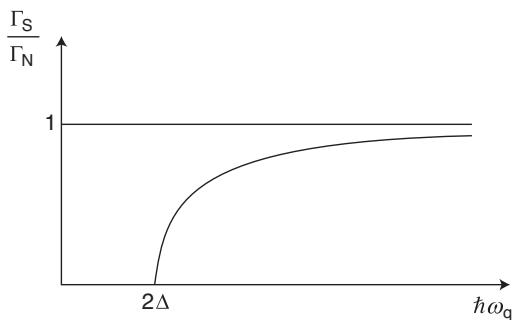
\includegraphics[width=0.55\textwidth]{figs/ch12/fig_12.20.jpg}
\caption*{图 12.20\quad 超导态电磁吸收与正常态电磁吸收之比。横轴为频率，$\Delta$ 为能隙能量。}\label{fig:auto:12.20}
\end{figure}

积分遍及自由粒子能量。因子 4 来自把积分下限从 $-\infty$ 换到零的转换。由于 $\Gamma_{\mathrm{s}}>0$，积分必须对所有的 $\varepsilon$ 与 $\varepsilon'$ 都为正。我们立即看到 $\varepsilon\varepsilon'>\Delta^{2}$，或等价地 $\hbar\omega_{\mathbf{q}}>2\Delta$。因此，当 $\hbar\omega_{\mathbf{q}}<2\Delta$ 时 $\Gamma_{\mathrm{s}}$ 必为零。这就是本节的主要结果。

通过变量替换可以得到更定量的预言。注意由于 $\varepsilon=(\epsilon^{2}+\Delta^{2})^{1/2}$，有 $\varepsilon\,\mathrm{d}\varepsilon=\epsilon\,\mathrm{d}\epsilon$。这一变量替换在 $\varepsilon$ 与 $\varepsilon'$ 的积分范围上引入了一个下限截断：
\begin{equation*}
\Gamma_{\mathrm{s}}=\mathrm{const.}\int_{\Delta}^{\infty}\mathrm{d}\varepsilon\int_{\Delta}^{\infty}\mathrm{d}\varepsilon'\,\delta\left(\varepsilon+\varepsilon'-\hbar\omega_{\mathbf{q}}\right)\frac{\left(\varepsilon\varepsilon'-\Delta^{2}\right)}{\left(\varepsilon^{\prime 2}-\Delta^{2}\right)^{1/2}\left(\varepsilon^{2}-\Delta^{2}\right)^{1/2}}\tag{12.279}
\end{equation*}
$\delta$ 函数约束 $\varepsilon'-\hbar\omega_{\mathbf{q}}=-\varepsilon$ 使我们能把 $\varepsilon$ 积分改写为
\begin{equation*}
\Gamma_{\mathrm{s}}=\mathrm{const.}\int_{\Delta}^{\hbar\omega_{\mathbf{q}}-\Delta}\mathrm{d}\varepsilon\,\frac{\varepsilon\left(\hbar\omega_{\mathbf{q}}-\varepsilon\right)-\Delta^{2}}{\left(\varepsilon^{2}-\Delta^{2}\right)^{1/2}\left(\left(\hbar\omega_{\mathbf{q}}-\varepsilon\right)^{2}-\Delta^{2}\right)^{1/2}},\tag{12.280}
\end{equation*}
其中我们把积分上限近似取为下界 $\hbar\omega_{\mathbf{q}}-\Delta$。当 $\Delta=0$ 时，被积函数化为常数，$\Gamma_{\mathrm{s}}\to\mathrm{const.}\,\hbar\omega_{\mathbf{q}}$。若把 $\Gamma_{\mathrm{s}}$ 的 $\Delta=0$ 值记为 $\Gamma_{\mathrm{N}}$ 并绘出 $\Gamma_{\mathrm{s}}/\Gamma_{\mathrm{N}}$，便得到图 12.20 所示的结果。我们在此导出的 $\Gamma_{\mathrm{s}}$ 形式与实验符合得很好。

\subsection{超声衰减}

现在考虑一束声子入射到超导体上的问题。我们曾经预告，除非入射声子束的能量超过 $2\Delta$，超导体对声子吸收应当是透明的。为证明这一点，我们用准粒子算符重写电子–声子哈密顿量，即式 (12.23)：
\begin{align*}
H_{\mathrm{e}\text{-}\mathrm{ph}}=\sum_{\mathbf{p},\mathbf{q}}^{\prime}M_{\mathbf{q}}\left(b_{\mathbf{q}}+b_{-\mathbf{q}}^{\dagger}\right)\Big[\big(u_{\mathbf{p}+\mathbf{q}}\gamma_{\mathbf{p}+\mathbf{q}\uparrow}^{\dagger}+v_{\mathbf{p}+\mathbf{q}}\gamma_{-(\mathbf{p}+\mathbf{q})\downarrow}\big)\big(u_{\mathbf{p}}\gamma_{\mathbf{p}\uparrow}+v_{\mathbf{p}}\gamma_{-\mathbf{p}\downarrow}^{\dagger}\big)\\
+\big(u_{-(\mathbf{p}+\mathbf{q})}\gamma_{\mathbf{p}+\mathbf{q}\downarrow}^{\dagger}-v_{-(\mathbf{p}+\mathbf{q})}\gamma_{-(\mathbf{p}+\mathbf{q})\uparrow}\big)\big(u_{-\mathbf{p}}\gamma_{\mathbf{p}\downarrow}-v_{-\mathbf{p}}\gamma_{-\mathbf{p}\uparrow}^{\dagger}\big)\Big],\tag{12.281}
\end{align*}
其中用到式 (12.245) 与式 (12.246)。准粒子–声子耦合产生两类不同的项：（1）单准粒子激发；（2）准粒子对的产生与湮没。单准粒子的产生与湮没过程
\begin{align*}
H_{\mathrm{e}\text{-}\mathrm{ph}}^{\mathrm{qp}}=\sum_{\mathbf{p},\mathbf{q}}^{\prime}M_{\mathbf{q}}\left(b_{\mathbf{q}}+b_{-\mathbf{q}}^{\dagger}\right)\Big[u_{\mathbf{p}+\mathbf{q}}u_{\mathbf{p}}\gamma_{\mathbf{p}+\mathbf{q}\uparrow}^{\dagger}\gamma_{\mathbf{p}\uparrow}+v_{\mathbf{p}+\mathbf{q}}v_{\mathbf{p}}\gamma_{-(\mathbf{p}+\mathbf{q})\downarrow}\gamma_{-\mathbf{p}\downarrow}^{\dagger}\\
+u_{-(\mathbf{p}+\mathbf{q})}u_{-\mathbf{p}}\gamma_{\mathbf{p}+\mathbf{q}\downarrow}^{\dagger}\gamma_{\mathbf{p}\downarrow}+v_{-(\mathbf{p}+\mathbf{q})}v_{-\mathbf{p}}\gamma_{-(\mathbf{p}+\mathbf{q})\uparrow}\gamma_{-\mathbf{p}\uparrow}^{\dagger}\Big],\tag{12.282}
\end{align*}
来自共轭的 $\gamma_{\mathbf{p}},\gamma_{\mathbf{p}'}^{\dagger}$ 对。附加的散射通道
\begin{align*}
H_{\mathrm{e}\text{-}\mathrm{ph}}^{\mathrm{pair}}=\sum_{\mathbf{p},\mathbf{q}}M_{\mathbf{q}}\left(b_{\mathbf{q}}+b_{-\mathbf{q}}^{\dagger}\right)\big[u_{\mathbf{p}+\mathbf{q}}v_{\mathbf{p}}\gamma_{\mathbf{p}+\mathbf{q}\uparrow}^{\dagger}\gamma_{-\mathbf{p}\downarrow}^{\dagger}-u_{-(\mathbf{p}+\mathbf{q})}v_{-\mathbf{p}}\gamma_{\mathbf{p}+\mathbf{q}\downarrow}^{\dagger}\gamma_{-\mathbf{p}\uparrow}^{\dagger}\\
+v_{\mathbf{p}+\mathbf{q}}u_{\mathbf{p}}\gamma_{-(\mathbf{p}+\mathbf{q})\downarrow}\gamma_{\mathbf{p}\uparrow}-v_{-(\mathbf{p}+\mathbf{q})}u_{-\mathbf{p}}\gamma_{-(\mathbf{p}+\mathbf{q})\uparrow}\gamma_{\mathbf{p}\downarrow}\big],\tag{12.283}
\end{align*}
则由准粒子对的产生与湮没来传递。

声子在超导体中被激发时，预期两类过程都会发生。然而，与电磁吸收问题一样，对的产生与湮没预期仅在 $\hbar\omega_{\mathbf{q}}>2\Delta$ 时出现。因为我们的目标是证明频率低于 $2\Delta$ 时声子吸收受到衰减，所以可以忽略配对散射项。于是我们专门考虑 $\hbar\omega_{\mathbf{q}}<\Delta$ 的情形，此时只有单粒子散射对跃迁振幅有贡献。发射项与吸收项的两种代表性类别示于图 12.21(a) 与 12.21(b)。每一项对 $\downarrow$ 与 $\uparrow$ 电子态的贡献相同。先考虑发射。描写单准粒子交换中声子发射的算符是
\begin{equation*}
V_{\mathrm{emiss}}^{\mathrm{qp}}=M_{\mathbf{q}}b_{-\mathbf{q}}^{\dagger}\left(u_{\mathbf{p}+\mathbf{q}}u_{\mathbf{p}}\gamma_{\mathbf{p}+\mathbf{q}\sigma}^{\dagger}\gamma_{\mathbf{p}\sigma}+v_{-(\mathbf{p}+\mathbf{q})}v_{-\mathbf{p}}\gamma_{\mathbf{p}\sigma}\gamma_{\mathbf{p}+\mathbf{q}\sigma}^{\dagger}\right),\tag{12.284}
\end{equation*}
其中我们在式 (12.282) 的第二项中作了 $-\mathbf{p}\to\mathbf{p}$ 与 $-\mathbf{p}-\mathbf{q}\to\mathbf{p}$ 的替换。利用诸 $\gamma$ 的反对易关系，可以把发射项改写为
\begin{equation*}
V_{\mathrm{emiss}}^{\mathrm{qp}}=M_{\mathbf{q}}b_{-\mathbf{q}}^{\dagger}\left[\left(u_{\mathbf{p}+\mathbf{q}}u_{\mathbf{p}}-v_{-(\mathbf{p}+\mathbf{q})}v_{-\mathbf{p}}\right)\gamma_{\mathbf{p}+\mathbf{q}\sigma}^{\dagger}\gamma_{\mathbf{p}\sigma}+v_{-(\mathbf{p}+\mathbf{q})}v_{-\mathbf{p}}\delta_{\mathbf{p},\mathbf{p}+\mathbf{q}}\right].\tag{12.285}
\end{equation*}
最后一项要求 $\mathbf{p}=\mathbf{p}+\mathbf{q}$，等价地 $\mathbf{q}=0$。然而 $M_{\mathbf{q}}$ 线性于 $\mathbf{q}$，故在 $\mathbf{q}=0$ 时为零。在发射过程中，末态的复合电子–声子态必须包含动量为 $\mathbf{q}$ 的声子以及动量为 $\mathbf{p}+\mathbf{q}$、自旋为 $\sigma$ 的准粒子。动量为 $\mathbf{p}$ 的准粒子不出现在这个态中。

\begin{figure}[H]\centering
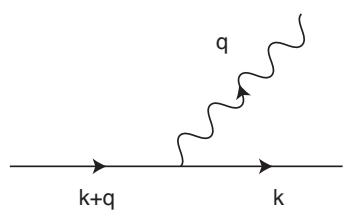
\includegraphics[width=0.42\textwidth]{figs/ch12/fig_12.21_a.jpg}\hfill
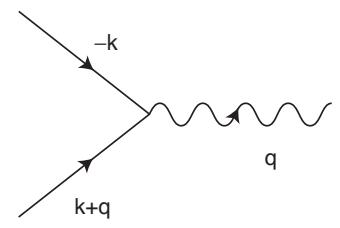
\includegraphics[width=0.4\textwidth]{figs/ch12/fig_12.21_b.jpg}\\[8pt]
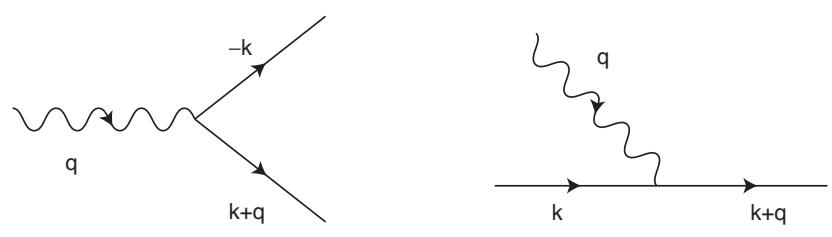
\includegraphics[width=0.82\textwidth]{figs/ch12/fig_12.21_c.jpg}
\caption*{图 12.21\quad 对超声衰减有贡献的 (a) 发射过程与 (b) 吸收过程。波浪线表示准粒子–声子相互作用。}\label{fig:auto:12.21}
\end{figure}

初态一般是包含任意数目准粒子（特别是动量为 $\mathbf{p}$、自旋为 $\sigma$ 的准粒子）的某个行列式态。令 $|\mathbf{p}+\mathbf{q}\sigma,\mathbf{q}\rangle$ 与 $|\mathbf{p}\sigma\rangle$ 分别为末态与初态。发射矩阵元简化为
\begin{equation*}
\langle\mathbf{p}+\mathbf{q}\sigma,\mathbf{q}|V_{\mathrm{emiss}}^{\mathrm{qp}}|\mathbf{p}\sigma\rangle=M_{\mathbf{q}}\left(u_{\mathbf{p}+\mathbf{q}}u_{\mathbf{p}}-v_{-(\mathbf{p}+\mathbf{q})}v_{-\mathbf{p}}\right)\sqrt{N_{\mathbf{q}}+1}\sqrt{n_{\mathbf{p}}\left(1-n_{\mathbf{p}+\mathbf{q}}\right)},\tag{12.286}
\end{equation*}
其中 $n_{\mathbf{p}}$ 是动量态 $\mathbf{p}$ 中准粒子的占据数。于是，同时计入 $\uparrow$ 与 $\downarrow$ 两种自旋后，发射的费米黄金规则速率为
\begin{align*}
\Gamma_{\mathrm{emiss}}^{\mathrm{qp}}&=\frac{2}{\hbar}\sum_{\mathbf{p}}\left(N_{\mathbf{q}}+1\right)\left|M_{\mathbf{q}}\right|^{2}\left(u_{\mathbf{p}+\mathbf{q}}u_{\mathbf{p}}-v_{\mathbf{p}+\mathbf{q}}v_{\mathbf{p}}\right)^{2}\\
&\quad\times n_{\mathbf{p}}\left(1-n_{\mathbf{p}+\mathbf{q}}\right)2\pi\delta\left(\hbar\omega_{\mathbf{q}}+\varepsilon_{\mathbf{p}}-\varepsilon_{\mathbf{p}+\mathbf{q}}\right).\tag{12.287}
\end{align*}
类似的论证可以应用于声子的吸收。跃迁速率的形式有两个主要差异。其一，因子 $N_{\mathbf{q}}+1$ 被换成 $N_{\mathbf{q}}$；这一变化源于吸收情形下末态少一个声子。其二，初态与末态分别形如 $|\mathbf{p}\sigma,\mathbf{q}\rangle$ 与 $|\mathbf{p}+\mathbf{q}\sigma\rangle$。所有这类初、末态之间的吸收速率
\begin{equation*}
\Gamma_{\mathrm{abs}}^{\mathrm{qp}}=\frac{2}{\hbar}\sum_{\mathbf{q}}N_{\mathbf{q}}|M_{\mathbf{q}}|\left(u_{\mathbf{p}+\mathbf{q}}u_{\mathbf{p}}-v_{\mathbf{p}+\mathbf{q}}v_{\mathbf{p}}\right)^{2}n_{\mathbf{p}+\mathbf{q}}\left(1-n_{\mathbf{p}}\right)2\pi\delta\left(\hbar\omega_{\mathbf{q}}+\varepsilon_{\mathbf{p}}-\varepsilon_{\mathbf{p}+\mathbf{q}}\right),\tag{12.288}
\end{equation*}
是各个速率之和，我们在费米黄金规则的层次上处理。

发射速率与吸收速率之差
\begin{align*}
\Gamma_{\mathbf{q}}&=\Gamma_{\mathrm{abs}}^{\mathrm{qp}}-\Gamma_{\mathrm{emiss}}^{\mathrm{qp}}\\
&=\frac{2}{\hbar}\sum_{\mathbf{p}}^{\prime}\left|M_{\mathbf{q}}\right|^{2}\left(u_{\mathbf{p}+\mathbf{q}}u_{\mathbf{p}}-v_{\mathbf{p}+\mathbf{q}}v_{\mathbf{p}}\right)^{2}2\pi\delta\left(\hbar\omega_{\mathbf{q}}+\varepsilon_{\mathbf{p}}-\varepsilon_{\mathbf{p}+\mathbf{q}}\right)\\
&\quad\times\left[N_{\mathbf{q}}\left(n_{\mathbf{p}+\mathbf{q}}-n_{\mathbf{p}}\right)-n_{\mathbf{p}}\left(1-n_{\mathbf{p}+\mathbf{q}}\right)\right],\tag{12.289}
\end{align*}
包含一个通过 $N_{\mathbf{q}}$ 依赖于声子占据的部分和一个不依赖的部分。在合并吸收项与发射项时，我们利用了相干因子的时间反演不变性。不依赖声子占据的部分定义了有效自发发射速率，而第一项定义了 $N_{\mathbf{q}}$ 个声子被吸收的总速率。于是我们定义
\begin{align*}
\frac{\mathrm{d}N_{\mathbf{q}}}{\mathrm{d}t}&=-\frac{2}{\hbar}\sum_{\mathbf{p}}\left|M_{\mathbf{q}}\right|^{2}\left(u_{\mathbf{p}+\mathbf{q}}u_{\mathbf{p}}-v_{\mathbf{p}+\mathbf{q}}v_{\mathbf{p}}\right)^{2}2\pi\delta\left(\hbar\omega_{\mathbf{q}}+\varepsilon_{\mathbf{p}}-\varepsilon_{\mathbf{p}+\mathbf{q}}\right)N_{\mathbf{q}}\left(n_{\mathbf{p}+\mathbf{q}}-n_{\mathbf{p}}\right)\\
&=-\alpha_{\mathbf{q}}N_{\mathbf{q}}\tag{12.290}
\end{align*}
为净声学衰减速率。

为求出 $\alpha_{\mathbf{q}}$，我们把求和化为积分
\begin{align*}
\alpha_{\mathbf{q}}&=\frac{4\pi}{\hbar}\left|M_{\mathbf{q}}\right|^{2}g^{2}(0)\int\mathrm{d}\epsilon_{\mathbf{p}}\,\mathrm{d}\epsilon_{\mathbf{p}'}\left(u_{\mathbf{p}}u_{\mathbf{p}'}-v_{\mathbf{p}}v_{\mathbf{p}'}\right)\left(n_{\mathbf{p}'}-n_{\mathbf{p}}\right)\\
&\quad\times\delta\left(\hbar\omega_{\mathbf{q}}+\varepsilon_{\mathbf{p}}-\varepsilon_{\mathbf{p}'}\right)\int\frac{\mathrm{d}\Omega_{\mathbf{p}}}{4\pi}\frac{\mathrm{d}\Omega_{\mathbf{p}'}}{4\pi}\,\delta\left(\mathbf{p}-\mathbf{p}'-\mathbf{q}\right)\tag{12.291}
\end{align*}
其中动量守恒由角度因子 $\delta\left(\mathbf{p}-\mathbf{p}'-\mathbf{q}\right)$ 保证。为简化式 (12.291)，注意角度因子在正常态与超导态中是相同的。由于假定能隙各向同性，可以把角度依赖分离出来；记该因子为 $A_{\Omega}$。现在我们需要相干因子的表达式：
\begin{equation*}
\left(u_{\mathbf{p}}u_{\mathbf{p}'}-v_{\mathbf{p}}v_{\mathbf{p}'}\right)^{2}=\frac{1}{2\varepsilon_{\mathbf{p}}\varepsilon_{\mathbf{p}'}}\left[\varepsilon_{\mathbf{p}}\varepsilon_{\mathbf{p}'}+\epsilon_{\mathbf{p}}\epsilon_{\mathbf{p}'}-\Delta^{2}\right],\tag{12.292}
\end{equation*}
其中已假定能隙为常数，$\Delta=\Delta_{\mathbf{p}}=\Delta_{\mathbf{p}'}$。注意 $n_{\mathbf{p}}$ 与 $\varepsilon_{\mathbf{p}}$ 都是 $\epsilon_{\mathbf{p}}$ 的偶函数。因此，对线性因子 $\epsilon_{\mathbf{p}}\epsilon_{\mathbf{p}'}$ 的积分因积分限为偶而消失。作为进一步的简化，注意到 $\mathrm{d}\varepsilon_{\mathbf{p}}/\mathrm{d}\epsilon_{\mathbf{p}}=\varepsilon_{\mathbf{p}}/\epsilon_{\mathbf{p}}$，我们把积分变量从 $\epsilon_{\mathbf{p}}$ 换成 $\varepsilon_{\mathbf{p}}$。剩下
\begin{align*}
\alpha_{\mathbf{q}}&=\frac{8\pi}{\hbar}\left|M_{\mathbf{q}}\right|^{2}g^{2}(0)A_{\Omega}\int_{\Delta}^{\infty}\mathrm{d}\varepsilon_{\mathbf{p}}\int_{\Delta}^{\infty}\mathrm{d}\varepsilon_{\mathbf{p}'}\,\frac{\varepsilon_{\mathbf{p}}\varepsilon_{\mathbf{p}'}}{\epsilon_{\mathbf{p}}\epsilon_{\mathbf{p}'}}\left(1-\frac{\Delta^{2}}{\varepsilon_{\mathbf{p}}\varepsilon_{\mathbf{p}'}}\right)\\
&\quad\times\left(n_{\mathbf{p}'}-n_{\mathbf{p}}\right)\delta\left(\hbar\omega_{\mathbf{q}}+\varepsilon_{\mathbf{p}}-\varepsilon_{\mathbf{p}'}\right).\tag{12.293}
\end{align*}
量 $N(0)\,\mathrm{d}\epsilon_{\mathbf{p}}/\mathrm{d}\varepsilon_{\mathbf{p}}=N(0)\varepsilon_{\mathbf{p}}/\epsilon_{\mathbf{p}}$ 大致就是准粒子激发的态密度。在费米面上，$\epsilon_{\mathbf{p}}\to 0$，$\mathrm{d}\epsilon_{\mathbf{p}}/\mathrm{d}\varepsilon_{\mathbf{p}}\to\infty$。但在积分范围内，$\varepsilon_{\mathbf{p}}/\epsilon_{\mathbf{p}}$ 是有限的。在 $\hbar\omega_{\mathbf{q}}\ll\Delta$ 的极限下，$\varepsilon_{\mathbf{p}'}\approx\varepsilon_{\mathbf{p}}$。因此，
\begin{equation*}
\frac{\varepsilon_{\mathbf{p}}}{\epsilon_{\mathbf{p}}}\frac{\varepsilon_{\mathbf{p}'}}{\epsilon_{\mathbf{p}'}}\left(1-\frac{\Delta^{2}}{\varepsilon_{\mathbf{p}}\varepsilon_{\mathbf{p}'}}\right)\to\frac{\varepsilon_{\mathbf{p}}^{2}}{\epsilon_{\mathbf{p}}^{2}}\left(\frac{\varepsilon_{\mathbf{p}}^{2}-\Delta^{2}}{\varepsilon_{\mathbf{p}}^{2}}\right)=1.\tag{12.294}
\end{equation*}

\begin{figure}[H]\centering
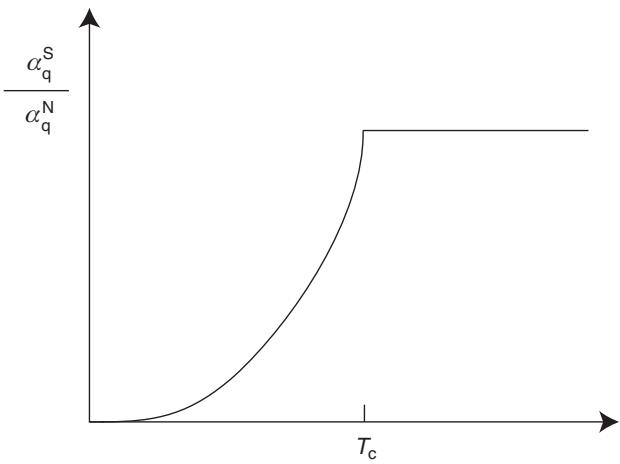
\includegraphics[width=0.55\textwidth]{figs/ch12/fig_12.22.jpg}
\caption*{图 12.22\quad 式 (12.297) 预言的超导态与正常态超声衰减之比。该比值在超导态中的下降是库珀对形成的一个标志。}\label{fig:auto:12.22}
\end{figure}

在这个极限下工作是完全合理的，因为我们考虑的只是单准粒子激发导致的声子吸收。在被积函数中取 $\varepsilon_{\mathbf{p}'}=\varepsilon_{\mathbf{p}}+\hbar\omega_{\mathbf{q}}$，我们得到
\begin{align*}
\alpha_{\mathbf{q}}&=\frac{8\pi}{\hbar}\left|M_{\mathbf{q}}\right|^{2}g^{2}(0)A_{\Omega}\int_{\Delta}^{\infty}\mathrm{d}\varepsilon_{\mathbf{p}}\left(n\left(\varepsilon_{\mathbf{p}}+\hbar\omega_{\mathbf{q}}\right)-n\left(\varepsilon_{\mathbf{p}}\right)\right)\\
&\simeq-\frac{8\pi}{\hbar}\left|M_{\mathbf{q}}\right|^{2}g^{2}(0)A_{\Omega}\hbar\omega_{\mathbf{q}}n(\Delta).\tag{12.295}
\end{align*}
正常态中 $\Delta=0$，于是
\begin{equation*}
\alpha_{\mathbf{q}}^{\mathrm{N}}=-\frac{8\pi}{\hbar}\left|M_{\mathbf{q}}\right|^{2}g^{2}(0)A_{\Omega}\hbar\omega_{\mathbf{q}}n(0)=-\frac{4\pi}{\hbar}\left|M_{\mathbf{q}}\right|^{2}g^{2}(0)A_{\Omega}\hbar\omega_{\mathbf{q}}.\tag{12.296}
\end{equation*}
比值 $\alpha_{\mathbf{q}}^{\mathrm{s}}/\alpha_{\mathbf{q}}^{\mathrm{N}}$ 约化为
\begin{equation*}
\frac{\alpha_{\mathbf{q}}^{\mathrm{s}}}{\alpha_{\mathbf{q}}^{\mathrm{N}}}=\frac{2}{\mathrm{e}^{\beta\Delta(T)}+1}.\tag{12.297}
\end{equation*}
$T=T_{\mathrm{c}}$ 时 $\Delta=0$，该比值给出 1，如图 12.22 所示。超声衰减率的这一计算（文献 [S1964]）与实验结果符合得极好。这里我们再次看到，最终决定超导态中声波吸收的仍然是能隙。当然，这一计算只对纵声子有效。在纵波情形中，$M_{\mathbf{q}}$ 在正常态与超导态中是相同的；而对于横声子，$M_{\mathbf{q}}$ 从正常态到超导态会发生剧烈变化。此时 $M_{\mathbf{q}}$ 的磁性依赖导致 $T=T_{\mathrm{c}}$ 处衰减率发生不连续的骤降，如图 12.23 所示（文献 [S1964]）。

\begin{figure}[H]\centering
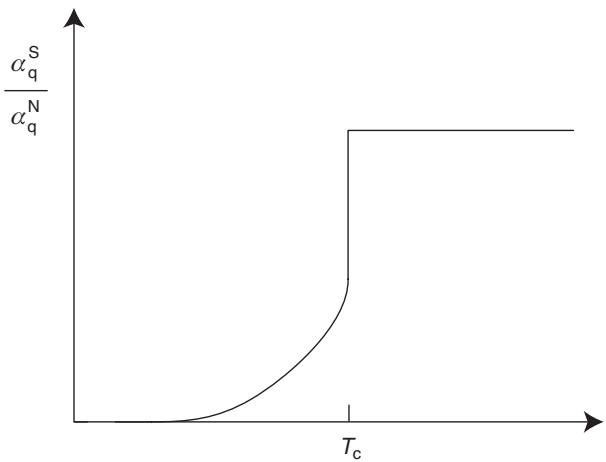
\includegraphics[width=0.55\textwidth]{figs/ch12/fig_12.23.jpg}
\caption*{图 12.23\quad 横声子的超导态与正常态超声吸收速率之比随温度 $T$ 的变化。}\label{fig:auto:12.23}
\end{figure}

\subsection{自旋–晶格弛豫}

我们利用 BCS 相干因子给出的最后一个计算，是自旋–晶格弛豫时间 $T_{1}$ 的计算。出于历史原因，这是一个关键性的计算，因为 $1/T_{1}$ 的峰应出现在 $T_{\mathrm{c}}$ 稍下方，这一预言比 Hebel 与 Slichter 的实验（文献 [HS1959]）更早。事实上，$1/T_{1}$ 在 $T_{\mathrm{c}}$ 稍下方增强的实验证实，是使 BCS 理论获得广泛接受的决定性证据。为定义 $T_{1}$，考虑对一集核自旋施加磁场。磁场撤去之后，自旋将弛豫回去以达到平衡磁化。这一过程所需的时间就称为 $T_{1}$。在绝缘体中，是原子核与电子杂质之间的耦合使核得以弛豫。听其自然，原子核无法达到平衡自旋温度。晶格温度必须由某种媒介传递给原子核。在金属中，提供这一耦合的是传导电子。由于超导体中的电子被锁定在相干态中，我们预期 $T_{1}$ 会被剧烈改变。考虑位于原点 $\mathbf{r}=0$ 处、磁矩为 $\mathbf{S}_{\mathrm{N}}$ 的原子核。$\mathbf{r}=0$ 处的净电子自旋由该处的局域电子自旋密度 $\mathbf{S}=\hbar\Psi^{\dagger}(0)\sigma\Psi(0)/2$ 给出，其中 $\Psi(0)$ 是 $\mathbf{r}=0$ 处的电子波函数，$\sigma$ 是泡利自旋矩阵。费米接触项
\begin{equation*}
H_{\mathrm{int}}=\frac{8\pi}{3}\mu_{\mathrm{B}}\mathbf{S}_{\mathrm{N}}\cdot\mathbf{S},\tag{12.298}
\end{equation*}
定义了 $\mathbf{r}=0$ 处原子核与电子之间的耦合。式 (12.298) 中的 $\mu_{\mathrm{B}}$ 是玻尔磁子。

要把这一耦合用于超导体中 $T_{1}$ 的计算，只需用准粒子算符表示 $\mathbf{S}$。为此，引入旋量场算符
\begin{equation*}
\Psi(\mathbf{r})=\frac{1}{\sqrt{V}}\sum_{\mathbf{p}}\mathrm{e}^{\mathrm{i}\mathbf{p}\cdot\mathbf{r}}\begin{pmatrix}a_{\mathbf{p}\uparrow}\\ a_{\mathbf{p}\downarrow}\end{pmatrix}.\tag{12.299}
\end{equation*}
在旋量记号下，原点处的局域电子自旋密度变为
\begin{equation*}
\mathbf{S}=\frac{\hbar}{2V}\sum_{\mathbf{p},\mathbf{p}'}\begin{pmatrix}a_{\mathbf{p}'\uparrow}^{\dagger} & a_{\mathbf{p}'\downarrow}^{\dagger}\end{pmatrix}\sigma\begin{pmatrix}a_{\mathbf{p}\uparrow}\\ a_{\mathbf{p}\downarrow}\end{pmatrix}.\tag{12.300}
\end{equation*}
现在我们用 $\Psi(\mathbf{r})$ 表示费米接触相互作用。因为乘积 $\mathbf{S}_{1}\cdot\mathbf{S}_{2}=S_{1}^{z}S_{2}^{z}+2\left(S_{1}^{+}S_{2}^{-}+S_{1}^{-}S_{2}^{+}\right)$，我们把费米接触项
\begin{equation*}
H_{\mathrm{int}}=\frac{4\pi}{3V}\mathbf{S}_{\mathrm{B}}^{\prime}\sum_{\mathbf{p},\mathbf{p}'}\mathbf{S}_{\mathrm{N}}^{z}\left(a_{\mathbf{p}'\uparrow}^{\dagger}a_{\mathbf{p}\uparrow}-a_{\mathbf{p}'\downarrow}^{\dagger}a_{\mathbf{p}\downarrow}\right)+2\mathbf{S}_{\mathrm{N}}^{+}a_{\mathbf{p}'\downarrow}^{\dagger}a_{\mathbf{p}\uparrow}+2\mathbf{S}_{\mathrm{N}}^{-}a_{\mathbf{p}'\uparrow}^{\dagger}a_{\mathbf{p}\downarrow},\tag{12.301}
\end{equation*}
写成熟悉的近藤形式，其中 $\mu_{\mathrm{B}}^{\prime}=\mu_{\mathrm{B}}/\hbar$（译注：式 (12.301) 中的系数 $\mathbf{S}_{\mathrm{B}}^{\prime}$ 原文如此排印，按上下文应为 $\mu_{\mathrm{B}}^{\prime}$）。

我们特别感兴趣的是核自旋被翻转的那些项。因此，可以专注于 $\mathbf{S}_{\mathrm{N}}^{-}$ 项或 $\mathbf{S}_{\mathrm{N}}^{+}$ 项。考虑 $\mathbf{S}_{\mathrm{N}}^{+}$。令 $H_{\mathrm{int}}^{+}$ 为核自旋向上翻转的那部分相互作用。这里我们再次引入准粒子表示
\begin{equation*}
a_{\mathbf{p}'\downarrow}^{\dagger}=u_{-\mathbf{p}'}\gamma_{\mathbf{p}'\downarrow}^{\dagger}-v_{-\mathbf{p}'}\gamma_{-\mathbf{p}'\uparrow}\tag{12.302}
\end{equation*}
以及
\begin{equation*}
a_{\mathbf{p}\uparrow}=u_{\mathbf{p}}\gamma_{\mathbf{p}\uparrow}+v_{\mathbf{p}}\gamma_{-\mathbf{p}\downarrow}^{\dagger},\tag{12.303}
\end{equation*}
于是 $H_{\mathrm{int}}^{+}$ 变换为
\begin{align*}
H_{\mathrm{int}}^{+}&=\frac{4\pi}{3V}\mu_{\mathrm{B}}^{\prime}\mathbf{S}_{\mathrm{N}}^{+}\sum_{\mathbf{p},\mathbf{p}'}\Big(u_{-\mathbf{p}'}u_{\mathbf{p}}\gamma_{\mathbf{p}'\downarrow}^{\dagger}\gamma_{\mathbf{p}\uparrow}-v_{-\mathbf{p}'}v_{\mathbf{p}}\gamma_{-\mathbf{p}'\uparrow}\gamma_{-\mathbf{p}\downarrow}^{\dagger}\\
&\quad-u_{\mathbf{p}}v_{-\mathbf{p}'}\gamma_{-\mathbf{p}'\uparrow}\gamma_{\mathbf{p}\uparrow}+u_{-\mathbf{p}'}v_{\mathbf{p}}\gamma_{\mathbf{p}'\downarrow}^{\dagger}\gamma_{-\mathbf{p}\downarrow}^{\dagger}\Big).\tag{12.304}
\end{align*}
前两项描写自旋相反的准粒子的产生与湮没，而后面的项则包含准粒子对的产生或湮没。典型情况下，核塞曼能量相对准粒子能隙能量很小。因此，如果我们专注于 $\hbar\omega\approx\mu_{\mathrm{B}}H$ 的频率范围（$H$ 为外磁场），则只有前者的项是相关的。我们的有效相互作用约化为
\begin{equation*}
H_{\mathrm{int}}^{+}\simeq\frac{4\pi}{3V}\mu_{\mathrm{B}}^{\prime}\mathbf{S}_{\mathrm{N}}^{+}\sum_{\mathbf{p},\mathbf{p}'}\left(u_{-\mathbf{p}'}u_{\mathbf{p}}\gamma_{\mathbf{p}'\downarrow}^{\dagger}\gamma_{\mathbf{p}\uparrow}+v_{-\mathbf{p}'}v_{\mathbf{p}}\gamma_{-\mathbf{p}\downarrow}^{\dagger}\gamma_{-\mathbf{p}'\uparrow}\right).\tag{12.305}
\end{equation*}
若初态形如 $|\mathbf{p}\uparrow,\mathbf{S}_{\mathrm{N}}^{z}\rangle$ 而末态为 $|\mathbf{p}\downarrow,\mathbf{S}_{\mathrm{N}}^{z}+1\rangle$，则该量的矩阵元非零。令 $\alpha_{\mathrm{N}}=\langle\mathbf{S}_{\mathrm{N}}^{z}+1|\mathbf{S}_{\mathrm{N}}^{+}|\mathbf{S}_{\mathrm{N}}^{z}\rangle$。所得的矩阵元
\begin{align*}
\Gamma_{\mathrm{SLR}}^{\mathbf{p}\mathbf{p}'}&=\frac{8\pi}{3}\mu_{\mathrm{B}}^{\prime}\alpha_{\mathrm{N}}\left(u_{-\mathbf{p}'}u_{\mathbf{p}}\sqrt{\left(1-n_{\mathbf{p}'\downarrow}\right)n_{\mathbf{p}\uparrow}}+v_{-\mathbf{p}'}v_{\mathbf{p}}\sqrt{\left(1-n_{-\mathbf{p}\downarrow}\right)n_{-\mathbf{p}'\uparrow}}\right)\\
&=\frac{4\pi}{3}\mu_{\mathrm{B}}^{\prime}\alpha_{\mathrm{N}}\left(u_{-\mathbf{p}'}u_{\mathbf{p}}+v_{-\mathbf{p}'}v_{\mathbf{p}}\right)\sqrt{\left(1-n_{\mathbf{p}'\downarrow}\right)n_{\mathbf{p}\uparrow}}\tag{12.306}
\end{align*}
导致核自旋–晶格弛豫速率
\begin{equation*}
T_{1}^{-1}=\frac{32\pi^{3}}{9\hbar}\mathbf{S}_{\mathrm{B}}^{2}\left|\alpha_{\mathrm{N}}\right|^{2}\sum_{\mathbf{p},\mathbf{p}'}\left(u_{-\mathbf{p}'}u_{\mathbf{p}}+v_{-\mathbf{p}'}v_{\mathbf{p}}\right)^{2}\left(1-n_{\mathbf{p}'\downarrow}\right)n_{\mathbf{p}\uparrow}\delta\left(\varepsilon_{\mathbf{p}'}-\varepsilon_{\mathbf{p}}\right).\tag{12.307}
\end{equation*}
（译注：式 (12.307) 中的 $\mathbf{S}_{\mathrm{B}}^{2}$ 原文如此排印，按式 (12.306) 应为 $\mu_{\mathrm{B}}^{\prime 2}$。）在这一理论层次上，我们当然忽略了近藤效应。超导体中磁性杂质的近藤区域确实是个微妙的问题，此处不予考虑。

从这里开始的步骤已是标准的：（1）引入态密度，把求和化为积分；（2）计算相干因子；（3）消去所有线性于裸能量的积分。由超声衰减的计算可知
\begin{equation*}
\left(u_{\mathbf{p}'}u_{\mathbf{p}}+v_{\mathbf{p}}v_{\mathbf{p}'}\right)^{2}=\frac{1}{2\varepsilon_{\mathbf{p}}\varepsilon_{\mathbf{p}'}}\left(\varepsilon_{\mathbf{p}}\varepsilon_{\mathbf{p}'}+\epsilon_{\mathbf{p}}\epsilon_{\mathbf{p}'}+\Delta_{\mathbf{p}}\Delta_{\mathbf{p}'}\right).\tag{12.308}
\end{equation*}
这里再次假定能隙为常数，于是弛豫速率约化为
\begin{align*}
T_{1}^{-1}&=\frac{64\pi^{3}}{9\hbar}\mu_{\mathrm{B}}^{\prime 2}\left|\alpha_{\mathrm{N}}\right|^{2}g^{2}(0)\int_{0}^{\infty}\mathrm{d}\epsilon_{\mathbf{p}}\int_{0}^{\infty}\mathrm{d}\epsilon_{\mathbf{p}'}\,n_{\mathbf{p}}\left(1-n_{\mathbf{p}'}\right)\left(\frac{\varepsilon_{\mathbf{p}}\varepsilon_{\mathbf{p}'}+\Delta^{2}}{\varepsilon_{\mathbf{p}}\varepsilon_{\mathbf{p}'}}\right)\delta\left(\varepsilon_{\mathbf{p}'}-\varepsilon_{\mathbf{p}}\right)\\
&=\frac{64\pi^{3}}{9\hbar}\mu_{\mathrm{B}}^{\prime 2}\left|\alpha_{\mathrm{N}}\right|^{2}g^{2}(0)\int_{\Delta}^{\infty}\mathrm{d}\varepsilon\,n(\varepsilon)\left(1-n(\varepsilon)\right)\frac{\varepsilon^{2}+\Delta^{2}}{\varepsilon^{2}+\Delta^{2}}.\tag{12.309}
\end{align*}
（译注：式 (12.309) 末行的分母 $\varepsilon^{2}+\Delta^{2}$ 原文如此排印，疑为排印之误。）$T=0$ 时乘积 $n(1-n)=0$，因为 $T=0$ 时 $n=1$。

$T=0$ 时，在 $\varepsilon=\pm\Delta$ 处存在发散。在 $\pm\Delta$ 附近，我们把被积函数写成
\begin{align*}
T_{1}^{-1}&\to\frac{64\pi^{3}}{9\hbar}\mu_{\mathrm{B}}^{\prime 2}\left|\alpha_{\mathrm{N}}\right|^{2}g^{2}(0)\int_{\Delta}^{\infty}\frac{\varepsilon^{2}+\Delta^{2}}{\varepsilon^{2}-\Delta^{2}}\,n(\varepsilon)\left(1-n(\varepsilon)\right)\mathrm{d}\varepsilon\\
&\propto\int_{\Delta}^{\infty}\frac{\varepsilon+\Delta}{\varepsilon-\Delta}\,\mathrm{d}\varepsilon,\tag{12.310}
\end{align*}
它是对数发散的。对数发散的系数正比于能隙 $\Delta$。这意味着对数发散从 $T=T_{\mathrm{c}}$ 处、即能隙开始出现之处启动。在实验中，由于能隙的动量依赖，能隙是各向异性的。因此，$T_{1}$ 的发散在可与 $\Delta$ 的平均值相比的范围内被略微抹平。Hebel 与 Slichter（文献 [HS1959]）最先观察到这一行为，如图 12.7 所示。

我们在微扰论的这一低阶下预言的对数发散，也许可以通过对所有更高阶项求和予以消除，或至少被展宽。因此，值得考察这一对数发散究竟有多稳固。电子–核相互作用的完整级数为
\begin{equation*}
\Gamma_{\mathrm{int}}^{\mathrm{full}}=\langle f|H_{\mathrm{int}}^{+}|i\rangle+\sum_{\mathbf{p}}\frac{\langle f|H_{\mathrm{int}}^{+}|\mathbf{p}\rangle\langle\mathbf{p}|H_{\mathrm{int}}^{+}|i\rangle}{E-\varepsilon_{\mathbf{p}}+\mathrm{i}\eta}+0(H^{3})+\cdots.\tag{12.311}
\end{equation*}
在局域磁矩问题的上下文中，我们把格林函数定义为
\begin{equation*}
G(E+\mathrm{i}\eta)=\sum_{\mathbf{p}}\frac{|\mathbf{p}\rangle\langle\mathbf{p}|}{E-\varepsilon_{\mathbf{p}}+\mathrm{i}\eta}.\tag{12.312}
\end{equation*}
示意性地，微扰级数形如
\begin{align*}
\Gamma_{\mathrm{int}}^{\mathrm{full}}&=\langle f|H_{\mathrm{int}}^{+}|i\rangle+\langle f|H_{\mathrm{int}}^{+}G\left(E+\mathrm{i}\eta\right)H_{\mathrm{int}}^{+}|i\rangle+\cdots\\
&=\left\langle f\left|\frac{H_{\mathrm{int}}^{+}}{1-H_{\mathrm{int}}^{+}G\left(E+\mathrm{i}\eta\right)}\right|i\right\rangle.\tag{12.313}
\end{align*}
为确定 $\Gamma_{\mathrm{int}}^{\mathrm{full}}$ 的发散部分，我们把格林函数中的求和化为积分：
\begin{align*}
G\left(E+\mathrm{i}\eta\right)&=N(0)\int\mathrm{d}\epsilon_{\mathbf{p}}\,\frac{1}{E-\varepsilon_{\mathbf{p}}+\mathrm{i}\eta}\\
&=N(0)\int_{\Delta}^{\infty}\left(\frac{\mathrm{d}\epsilon_{\mathbf{p}}}{\mathrm{d}\varepsilon_{\mathbf{p}}}\right)\frac{\mathrm{d}\varepsilon_{\mathbf{p}}}{E-\varepsilon_{\mathbf{p}}+\mathrm{i}\eta}.\tag{12.314}
\end{align*}
我们前面已经证明，$N(0)\,\mathrm{d}\epsilon_{\mathbf{p}}/\mathrm{d}\varepsilon_{\mathbf{p}}$ 定义了态密度
\begin{equation*}
\rho\left(\varepsilon_{\mathbf{p}}\right)=\frac{N(0)\varepsilon_{\mathbf{p}}}{\sqrt{\varepsilon_{\mathbf{p}}^{2}-\Delta_{\mathbf{p}}^{2}}}=N(0)\frac{\varepsilon_{\mathbf{p}}}{\epsilon_{\mathbf{p}}},\tag{12.315}
\end{equation*}
它在 $\varepsilon_{\mathbf{p}}=\Delta_{\mathbf{p}}$ 处发散。因此，
\begin{align*}
\lim_{\eta\to 0}G(E+\mathrm{i}\eta)&=\int_{\Delta}^{\infty}\rho(\varepsilon_{\mathbf{p}})\left[P\left(\frac{1}{E-\varepsilon_{\mathbf{p}}}\right)-\mathrm{i}\pi\delta\left(E-\varepsilon_{\mathbf{p}}\right)\right]\mathrm{d}\varepsilon_{\mathbf{p}}\\
&=\mathrm{Re}G-\mathrm{i}\pi\rho(E),\tag{12.316}
\end{align*}
而微扰级数变为
\begin{equation*}
\Gamma_{\mathrm{int}}^{\mathrm{full}}=\left\langle f\left|\frac{H_{\mathrm{int}}^{+}}{\left(1-H_{\mathrm{int}}^{+}\mathrm{Re}G\right)+\mathrm{i}\pi H_{\mathrm{int}}\rho(E)}\right|i\right\rangle.\tag{12.317}
\end{equation*}
在 $E=\Delta$ 附近，式 (12.317) 的分母由 $\rho(E)$ 项主导。在此极限下，$\Gamma_{\mathrm{int}}^{\mathrm{full}}\to 1/\left(\mathrm{i}\pi\rho(E)\right)$。这个量的平方恰好抵消了我们前面弛豫速率表达式中的发散项 $1/\left(\varepsilon_{\mathbf{p}}^{2}-\Delta^{2}\right)$。

为更清楚地看到这一点，我们把弛豫速率改写为
\begin{align*}
T_{1}^{-1}&=\frac{64\pi^{3}}{9\hbar}\mu_{\mathrm{B}}^{\prime 2}\left|\alpha_{\mathrm{N}}\right|^{2}g^{2}(0)\int_{\Delta}^{\infty}\mathrm{d}\varepsilon\,n(\varepsilon)\left(1-n(\varepsilon)\right)\left(\frac{\rho(\varepsilon)}{\varepsilon}\right)^{2}\\
&\quad\times\frac{\left(\varepsilon^{2}+\Delta^{2}\right)}{\left(1-H_{\mathrm{int}}^{+}\mathrm{Re}G\right)^{2}+\pi^{2}\left|H_{\mathrm{int}}^{+}\right|^{2}\rho^{2}(\varepsilon)},\tag{12.318}
\end{align*}
它约化为
\begin{equation*}
T_{1}^{-1}\propto\int_{\Delta}^{\infty}\mathrm{d}\varepsilon\,\left(1-n(\varepsilon)\right)n(\varepsilon)\frac{\varepsilon^{2}+\Delta^{2}}{\left(1+\pi^{2}\left|H_{\mathrm{int}}^{+}\right|^{2}g^{2}(0)\right)\varepsilon^{2}-\Delta^{2}}.\tag{12.319}
\end{equation*}
在导出式 (12.319) 时，我们忽略了格林函数的实部，因为就收敛性而言它没有实质作用。这个表达式在 $\varepsilon^{2}=\Delta^{2}$ 处完全收敛。事实上，由于 $\left(1+\pi^{2}|H_{\mathrm{int}}|^{2}g^{2}(0)\right)>1$，积分在整个积分范围内都不发散。因此，对微扰级数高阶项的求和，导致弛豫速率的峰在 $T_{\mathrm{c}}$ 紧下方被抹平。

\section{约瑟夫森隧穿}

考虑由一薄层绝缘势垒隔开的两个超导体。按直观的想象，在没有外加电压的情况下，除了单个准粒子或许能隧穿绝缘势垒之外，我们预期两个超导体之间不会有可观的电荷输运。约瑟夫森（文献 [J1962]）证明这种直观图像并不正确。特别地，他证明了对于足够薄的势垒，在没有外加电压时，库珀对会相干地在两个超导体之间流动，从而在势垒中建立起超流。此外，库珀对穿越势垒的输运不会在任一超导体中产生准粒子。当存在外加电压时，超流以确定的周期振荡。直流与交流约瑟夫森隧穿这两个效应的本质，都在于超导态中获得的相位相干性。

我们先关注直流约瑟夫森效应。考虑由薄绝缘势垒隔开的两个超导体。令 $H_{\mathrm{T}}$ 表示跨越薄势垒的单粒子隧穿哈密顿量。这一项的具体形式在此并不重要。唯一重要的特征是 $H_{\mathrm{T}}$ 每次只转移一个电子。一开始我们假设两个超导体之间没有电压差，因而它们处于同一化学势。我们可以通过类比紧束缚近似下一维周期链中的电子输运来导出约瑟夫森效应。在该近似中，每个格点上放置一个单轨道，跳跃项传递最近邻格点之间的输运。在这样的系统中，把一个电子输运过 $m$ 个格点不需要任何能量。同样，当两个超导体之间没有外加电压差时，把 $m$ 个库珀对移过势垒也不需要能量。令 $|\Phi_{2m}\rangle$ 表示 $2m$ 个库珀对被转移过势垒时的多体态。这些态的简并被单电子隧穿项 $H_{\mathrm{T}}$ 解除。因此，我们把系统的总态展开为所有此类对态的线性组合
\begin{equation*}
|\Psi_{\phi}\rangle\equiv|\phi\rangle=\sum_{m}\mathrm{e}^{2\mathrm{i}m\phi}|\Phi_{2m}\rangle\tag{12.320}
\end{equation*}
即对所有此类对态求和。相位 $\phi$ 扮演的角色，正如一维周期紧束缚模型中的波矢 $k$。如前所述，粒子数 $2m$ 与相位 $\phi$ 是共轭变量。

为计算隧穿过程造成的能量移动，我们采用微扰论。一阶项 $\langle\phi|H_{\mathrm{T}}|\phi\rangle$ 恒为零，因为 $\phi$ 是所有对态之和，而 $H_{\mathrm{T}}$ 是单体算符。因此，第一个非零项出现在二阶。令
\begin{equation*}
\widehat{H}_{\mathrm{T}}^{(2)}=\widehat{H}_{\mathrm{T}}\frac{|I\rangle\langle I|}{E-E_{\mathrm{I}}}\widehat{H}_{\mathrm{T}}\tag{12.321}
\end{equation*}
表示二阶的隧穿算符，其中 $E_{\mathrm{I}}$ 是中间态 $|I\rangle$ 的能量。能量的二阶修正
\begin{align*}
E_{\phi}&=\langle\phi|\widehat{H}_{\mathrm{T}}^{(2)}|\phi\rangle\\
&=\sum_{m,m'}\mathrm{e}^{2\mathrm{i}\phi(m-m')}\langle 2m'|\widehat{H}_{\mathrm{T}}^{(2)}|2m\rangle\\
&=\sum_{m}\left(\mathrm{e}^{2\mathrm{i}\phi}\langle 2m|\widehat{H}_{\mathrm{T}}^{(2)}|2(m+1)\rangle+\mathrm{e}^{-2\mathrm{i}\phi}\langle 2m|\widehat{H}_{\mathrm{T}}^{(2)}|2(m-1)\rangle\right),\tag{12.322}
\end{align*}
是所有相差一个库珀对的矩阵元之和。我们已经假定 $\langle\phi|\phi\rangle=1$。为简化此式，注意中间态的能量涉及粒子–空穴激发，故 $E_{\mathrm{I}}$ 必须至少比 $E$ 高出 $2\Delta$。因此 $E-E_{\mathrm{I}}<0$。若把隧穿项视为纯实数，能量移动便简化为
\begin{equation*}
E_{\phi}=-\frac{\hbar J_{0}}{2}\cos 2\phi,\tag{12.323}
\end{equation*}
其中
\begin{equation*}
\hbar J_{0}=4\sum_{m}\left|\langle 2m|\widehat{H}_{\mathrm{T}}^{(2)}|2(m+1)\rangle\right|.\tag{12.324}
\end{equation*}
能量移动中的负号来自激发能的符号。由哈密顿方程，即式 (12.170)，显然若能量移动依赖于相位，则势垒两侧的对数就会涨落。这一涨落完全源于隧穿过程。我们直接计算对电流，
\begin{equation*}
I=2e\frac{\mathrm{d}\langle 2m\rangle}{\mathrm{d}t}=2e\left\langle\frac{\mathrm{d}E_{\phi}}{\mathrm{d}\hbar\phi}\right\rangle=2eJ_{0}\sin 2\phi,\tag{12.325}
\end{equation*}
也就是对相位求能量移动的导数。因此，在没有外加电压时，有一直流超流流过势垒。电流的取值范围为 $-2eJ_{0}$ 到 $2eJ_{0}$。这种形式的超流由安德森与 Rowell（文献 [AR1963]）首次观察到。若势垒两端存在电势差 $V$，则哈密顿量中必须添加形如 $2mV$ 的项。因此，由哈密顿方程，即式 (12.170)，相位随时间按
\begin{equation*}
\frac{\mathrm{d}\langle\hbar\phi\rangle}{\mathrm{d}t}=2eV\tag{12.326}
\end{equation*}
涨落。这两条方程，即式 (12.325) 与式 (12.326)，共同完全确定了势垒间超流的行为。为作说明，考虑最简单的情形：电压 $V$ 不随时间变化。此时相位 $\phi$ 随时间线性变化，因而电流按 $\sin\left(2eVt/\hbar\right)$ 振荡。于是，有频率为 $2eV/\hbar$ 的交变电流流动。

\section*{小结}
\addcontentsline{toc}{section}{小结}

我们已经证明，BCS 的配对假设足以解释低温超导体的所有相关实验观测量。事实上，BCS 配对机制是目前唯一可用的、能够描述向超导态转变的理论。与低 $T_{\mathrm{c}}$ 材料不同，铜氧化物中的超导电性源于对绝缘体的掺杂。此外，该绝缘体具有部分填充的能带，因而属于莫特绝缘体之列——在这类体系中，输运的缺失源于电子间的强排斥。因此，我们事先（\emph{a priori}）就知道，即便只是描述其正常态性质，从费米液体理论出发也是不合理的。简言之，铜氧化物深刻的唯象学正蕴藏于掺杂莫特绝缘体的物理之中。对于这类体系，能否构建出像 BCS 理论那样简洁而透澈的解释，仍是一个悬而未决的问题。

\section*{习题}
\addcontentsline{toc}{section}{习题}

\textbf{习题 12.1}\quad 在金兹堡–朗道唯象方法的框架内，确定存在磁场时自由能密度的形式。证明超导态与正常态的自由能差由下式给出：
\begin{equation*}
F_{\mathrm{S}}-F_{\mathrm{N}}=-\frac{H_{\mathrm{c}}^{2}(T)}{8\pi}.\tag{12.327}
\end{equation*}

\textbf{习题 12.2}\quad 把金兹堡–朗道波函数写成 $\psi(\mathbf{r})=\sqrt{n(\mathbf{r})}\,\mathrm{e}^{\mathrm{i}\theta(\mathbf{r})}$，证明用变量 $\theta$ 与 $n(\mathbf{r})$ 表示的电流密度由下式给出：
\begin{equation*}
\mathbf{j}=\frac{e\hbar}{m}\left(\nabla\theta-\frac{e\mathbf{A}}{c\hbar}\right)n(\mathbf{r}).\tag{12.328}
\end{equation*}
然后设在材料的体内电流密度为零，因此 $\hbar\nabla\theta=e\mathbf{A}$。在超导环中沿一条闭合回路对该表达式两边积分，证明所包围的磁通是量子化的。对超导体而言，$e$ 的正确取值是什么？

\textbf{习题 12.3}\quad 直接用二阶微扰论证明电子–声子相互作用是负的，且由式 (12.34) 中的第二项给出。

\textbf{习题 12.4}\quad 就电子的三重态配对重做库珀对失稳的计算。

\textbf{习题 12.5}\quad 对一个单态库珀对计算 $\langle r^{2}\rangle$。

\textbf{习题 12.6}\quad 在 BCS 配对相互作用存在下超导态失稳的问题中，确定 $T\to T_{\mathrm{c}}$ 时对幅增长速率的形式。

\textbf{习题 12.7}\quad 计算对易子 $[b_{k},b_{k}^{\dagger}]$，其中诸 $b_{k}$ 是库珀对湮没算符。库珀对产生与湮没算符不对易意味着什么？

\textbf{习题 12.8}\quad 计算超导体中的平均粒子数。令 $|\Psi\rangle$ 表示 BCS 对态。证明在该对态中数算符 $N$ 的平均值为
\begin{equation*}
\langle\Psi|N|\Psi\rangle=\langle\Psi|\sum_{k,\sigma}a_{k\sigma}^{\dagger}a_{k\sigma}|\Psi\rangle=2\sum_{k}|v_{k}|^{2}\tag{12.329}
\end{equation*}
再计算涨落 $\langle\left(N-\langle N\rangle\right)^{2}\rangle$。你应得到一个只含 $u_{k}$ 与 $v_{k}$ 的简单结果。$u_{k}$ 与 $v_{k}$ 取什么特殊值时涨落最大？解释你的结果。

\textbf{习题 12.9}\quad 迄今我们忽略了能隙的任何空间不均匀性。考虑 $\Delta_{\mathbf{q}}=\Delta_{0}\mathrm{e}^{2\mathrm{i}\mathbf{q}\cdot\mathbf{r}}$ 形式的能隙，其中 $q\ll p_{\mathrm{F}}$。求 $\Delta_{0}$ 的新自洽条件。在 $T=0$ 时，证明对 $q<q_{\mathrm{c}}\approx\Delta_{0}/\hbar v_{\mathrm{F}}$，$\Delta$ 与 $q$ 无关。在 $T_{\mathrm{c}}$ 附近展开能隙方程，证明
\begin{equation*}
\frac{\Delta(T)}{k_{\mathrm{B}}T_{\mathrm{c}}}\approx\frac{8\pi^{2}}{7\zeta(3)}\left(1-T/T_{\mathrm{c}}\right)-\frac{2}{3}\left(\frac{\hbar^{2}p_{\mathrm{F}}}{mk_{\mathrm{B}}T_{\mathrm{c}}}\right)^{2}q^{2}.\tag{12.330}
\end{equation*}
然后确定使能隙为零的 $q$ 的临界值。

\textbf{习题 12.10}\quad 显式求出式 (12.260) 中的各求和，证明当 $T/T_{\mathrm{c}}\ll 1$ 时，$F_{\mathrm{N}}-F_{\mathrm{S}}\propto 1-\left(T/T_{\mathrm{c}}\right)^{2}$。

\textbf{习题 12.11}\quad 把一个安德森型杂质放入超导体。你要对该问题建立模型，并发展出局域磁矩形成的判据。可以应用若干假设。首先，在变换到准粒子基底时，忽略所有不守恒自旋与粒子数的项。问题至此应当是直截了当的。你应能完整地重做安德森问题。清楚地讨论局域磁矩何时存在、何时不存在。

\section*{参考文献}
\addcontentsline{toc}{section}{参考文献}

\begin{itemize}[leftmargin=2em,itemsep=0pt,parsep=0pt,label={}]
\item [A1957] A. A. Abrikosov, \emph{Sov. Phys. JETP} \textbf{5}, 1174 (1957).
\item [AR1963] P. W. Anderson and J. M. Rowell, \emph{Phys. Rev. Lett.} \textbf{10}, 230 (1963).
\item [BCS1957] J. Bardeen, L. N. Cooper, and J. R. Schrieffer, \emph{Phys. Rev.} \textbf{106}, 162 (1957); \textbf{108}, 1175 (1957).
\item [BG1990] G. Benefatto and G. Gallavotti, \emph{J. Stat. Phys.} \textbf{59}, 541 (1990).
\item [C1956] L. N. Cooper, \emph{Phys. Rev.} \textbf{104}, 1189 (1956).
\item [GL1950] G. V. L. Ginsburg and L. D. Landau, \emph{J. Exptl. Theor. Phys. (USSR)} \textbf{20}, 1064 (1950).
\item [GF1987] M. Gurvitch and A. T. Fiory, \emph{Phys. Rev. Lett.} \textbf{59}, 1337 (1987).
\item [HS1959] L. C. Hebel and C. P. Slichter, \emph{Phys. Rev.} \textbf{113}, 1504 (1959); L. C. Hebel, \emph{Phys. Rev.} \textbf{116}, 79 (1959).
\item [J1962] B. D. Josephson, \emph{Phys. Lett.} \textbf{1}, 251 (1962).
\item [L1956] L. D. Landau, \emph{Sov. Phys. JETP} \textbf{3}, 920 (1956); \textbf{8}, 70 (1959).
\item [L1964] A. I. Larkin, \emph{Sov. Phys. JETP} \textbf{19}, 1478 (1964).
\item [L1965] A. J. Leggett, \emph{Phys. Rev. Ser. A} \textbf{140}, 1869 (1965).
\item [P1992] J. Polchinski, arXiv:hep-th/9210046.
\item [SM1991] R. Shankar, \emph{Physica} \textbf{A177}, 530 (1991).
\item [S1964] J. R. Schrieffer, \emph{Theory of Superconductivity} (Benjamin, New York, 1964).
\end{itemize}
